\documentclass[11pt,a4paper]{article}
\usepackage[margin=1.8cm,top=2.5cm,bottom=2.2cm,headheight=24pt]{geometry}
\usepackage{fontspec}
\setmainfont{RakutenSerifApp}[
  Path = /home/sudheesh/.fonts/Notesnook/,
  Extension = .ttf,
  UprightFont = *-Regular,
  BoldFont = *-Bold,
  ItalicFont = *-Italic,
  BoldItalicFont = *-BoldItalic
]
\usepackage{amsmath,amssymb,mathtools}
\usepackage{booktabs,array,tabularx,multirow}
\usepackage{graphicx}
\graphicspath{{figures_mod1/}}
\usepackage{xcolor}
\usepackage{titlesec}
\usepackage{fancyhdr}
\usepackage{enumitem}
\usepackage{caption}
\usepackage{tcolorbox}
\tcbuselibrary{skins,breakable}
\usepackage{tikz}
\usepackage{pgfplots}
\pgfplotsset{compat=1.18}
\usetikzlibrary{arrows.meta,calc,positioning,patterns,decorations.pathmorphing}
\usepackage[hidelinks,pdfusetitle]{hyperref}

% Define custom column for tabularx
\newcolumntype{Y}{>{\centering\arraybackslash}X}

% Define color palette
\definecolor{navyprimary}{RGB}{15, 35, 65}
\definecolor{accentblue}{RGB}{2, 132, 199}
\definecolor{tealaccent}{RGB}{13, 148, 136}
\definecolor{cardbg}{RGB}{248, 250, 252}
\definecolor{cardborder}{RGB}{203, 213, 225}
\definecolor{calloutbg}{RGB}{241, 245, 249}
\definecolor{calloutframe}{RGB}{100, 116, 139}
\definecolor{formulabg}{RGB}{238, 242, 255}
\definecolor{formulaframe}{RGB}{99, 102, 241}
\definecolor{examplebg}{RGB}{250, 250, 250}
\definecolor{exampleframe}{RGB}{56, 189, 248}
\definecolor{highlightgold}{RGB}{180, 83, 9}
\definecolor{alertbg}{RGB}{254, 242, 242}
\definecolor{alertframe}{RGB}{239, 68, 68}

% Caption styling
\captionsetup{font=small,labelfont={bf,color=navyprimary},skip=5pt}

% Typography & Header/Footer
\pagestyle{fancy}
\fancyhf{}
\renewcommand{\headrulewidth}{0.6pt}
\renewcommand{\headrule}{\hbox to\headwidth{\color{navyprimary}\leaders\hrule height \headrulewidth\hfill}}
\fancyhead[L]{\small\bfseries\color{navyprimary}Power Electronics (Module 1) --- Master Study Guide}
\fancyhead[R]{\small\color{accentblue}CET S5 EEE}
\fancyfoot[L]{\small\color{gray}College of Engineering Trivandrum}
\fancyfoot[R]{\small\bfseries\color{navyprimary}Page \thepage}

% Section Titles Styling
\titleformat{\section}{\Large\bfseries\color{navyprimary}}{}{0em}{}[\vspace{1mm}{\color{accentblue}\hrule height 1.2pt}]
\titleformat{\subsection}{\large\bfseries\color{accentblue}}{}{0em}{}
\titleformat{\subsubsection}{\normalsize\bfseries\color{tealaccent}}{}{0em}{}

% Tcolorbox custom environments (Border-free modern cards with solid background colors)
\newtcolorbox{conceptbox}[1][]{
  enhanced,
  colback=calloutbg,
  colframe=calloutbg,
  colbacktitle=calloutbg,
  coltitle=navyprimary,
  fonttitle=\bfseries,
  title={#1},
  titlerule=0pt,
  boxrule=0pt,
  frame hidden,
  arc=2.5mm,
  left=4mm, right=4mm, top=3mm, bottom=3mm,
  breakable
}

\newtcolorbox{formulabox}[1][]{
  enhanced,
  colback=formulabg,
  colframe=formulabg,
  colbacktitle=formulabg,
  coltitle=navyprimary,
  fonttitle=\bfseries,
  title={#1},
  titlerule=0pt,
  boxrule=0pt,
  frame hidden,
  arc=2.5mm,
  left=4mm, right=4mm, top=3mm, bottom=3mm,
  breakable
}

\newtcolorbox{examplebox}[1][]{
  enhanced,
  colback=examplebg,
  colframe=examplebg,
  colbacktitle=examplebg,
  coltitle=navyprimary,
  fonttitle=\bfseries,
  title={#1},
  titlerule=0pt,
  boxrule=0pt,
  frame hidden,
  arc=2.5mm,
  left=4mm, right=4mm, top=3mm, bottom=3mm,
  middle=2.5mm,
  segmentation style={solid, draw=cardborder, line width=0.6pt},
  breakable
}

\newtcolorbox{alertbox}[1][]{
  enhanced,
  colback=alertbg,
  colframe=alertbg,
  colbacktitle=alertbg,
  coltitle=alertframe,
  fonttitle=\bfseries,
  title={#1},
  titlerule=0pt,
  boxrule=0pt,
  frame hidden,
  arc=2.5mm,
  left=4mm, right=4mm, top=3mm, bottom=3mm,
  breakable
}

% Remove black borders from \boxed formulas while keeping their prominent display
\renewcommand{\boxed}[1]{#1}

% Float placement parameters to prevent large blank spaces
\renewcommand{\topfraction}{0.90}
\renewcommand{\bottomfraction}{0.85}
\renewcommand{\textfraction}{0.10}
\renewcommand{\floatpagefraction}{0.75}
\setcounter{topnumber}{4}
\setcounter{bottomnumber}{4}
\setcounter{totalnumber}{8}
\raggedbottom

\begin{document}

% Title Header
\begin{center}
  {\huge\bfseries\color{navyprimary} POWER ELECTRONICS (PE) --- MODULE 1}\\[1.5ex]
  {\Large\bfseries\color{accentblue} The Definitive Master Study Guide, Device Physics Atlas \& Derivation Handbook}\\[1.5ex]
  {\normalsize\bfseries Course: B.Tech S5 Electrical \& Electronics Engineering (EEE) \quad|\quad College of Engineering Trivandrum (CET)}\\[0.8ex]
  {\small Integrated References: Dr. P. S. Bimbhra, Ned Mohan, Daniel W. Hart, L. Umanand, M. H. Rashid \& B. J. Baliga}
\end{center}
\vspace{-1em}
\noindent\textcolor{accentblue}{\rule{\textwidth}{1.5pt}}
\vspace{0.5em}

\tableofcontents
\newpage

%%%%%%%%%%%%%%%%%%%%%%%%%%%%%%%%%%%%%%%%%%%%%%%%%%%%%%%%%%%%%%%%%%%%%%%%%%%%%%%
\section{Foundations of Power Electronics \& Thermal Management}
%%%%%%%%%%%%%%%%%%%%%%%%%%%%%%%%%%%%%%%%%%%%%%%%%%%%%%%%%%%%%%%%%%%%%%%%%%%%%%%

\subsection{Scope, Motivation, and System Architecture}

Power Electronics is the branch of electrical and electronics engineering that deals with the efficient conversion, control, and conditioning of electric power using solid-state semiconductor switching devices. In contrast to signal electronics, where information fidelity and linear amplification are paramount, the defining objective of power electronics is \textbf{maximum energetic efficiency} ($\eta \to 100\%$), \textbf{minimal physical footprint} (high power density), \textbf{uncompromising reliability}, and \textbf{low system cost}.

Globally, over 80\% of all generated electrical energy is processed by at least one power electronic converter between the generation bus and the end-use terminal.

\subsubsection{Applications Classification of Power Electronics}
Power electronic converters form the technological foundation across the following application domains (frequently asked exam question):
\begin{enumerate}[leftmargin=*]
  \item \textbf{Commercial:} Uninterruptible Power Supplies (UPS), elevator drives, HVAC systems, lighting control.
  \item \textbf{Domestic:} Microwave ovens, washing machines, air conditioner compressors, induction cooktops, LED driver circuits.
  \item \textbf{Industrial:} Variable Frequency Drives (VFDs) for pumps, blowers, conveyors; DC motor speed control for steel rolling mills, paper mills; arc welding power supplies; electroplating rectifiers.
  \item \textbf{Telecom:} Switch-Mode Power Supplies (SMPS) for base stations, high-efficiency DC-DC converters for telecom rectifiers.
  \item \textbf{Aerospace:} Aircraft/spacecraft power management systems, avionics power supplies, electric actuation systems.
  \item \textbf{Transportation:} Electric/hybrid vehicle traction inverters ($100 - 300\text{ kW}$), railway traction systems, metro/maglev propulsion.
  \item \textbf{Utility / Power Systems:} High-Voltage DC (HVDC) transmission, Flexible AC Transmission Systems (FACTS), Static VAR Compensators (SVC), STATCOM, renewable energy grid integration (solar PV inverters, wind turbine converters).
\end{enumerate}

\subsubsection{Disadvantages of Power Electronics}
While power electronics enables high-efficiency power conversion, certain inherent limitations exist:
\begin{itemize}[leftmargin=*]
  \item \textbf{Harmonic Generation:} High-frequency switching generates significant current and voltage harmonics that distort AC mains waveforms, requiring passive ($LC$) or active harmonic filters.
  \item \textbf{Low Input Power Factor in AC-DC and AC-AC Converters:} Uncontrolled rectifiers draw highly distorted, non-sinusoidal currents with poor displacement power factor, requiring Power Factor Correction (PFC) circuits.
  \item \textbf{Electromagnetic Interference (EMI):} High $dv/dt$ and $di/dt$ switching transients radiate conducted and radiated EMI, necessitating EMI filters, shielding, and compliance with international standards (EN 55022, CISPR 11, FCC Part 15).
  \item \textbf{Low Overload Capacity:} Power semiconductor devices have strict thermal limits and cannot tolerate sustained overload currents (unlike transformers or rotating machines with thermal inertia). Fast-acting protection (electronic fuses, crowbars) is mandatory.
  \item \textbf{Complex Power Regeneration / Bidirectional Power Flow:} Implementing bidirectional energy flow (e.g., regenerative braking in EVs) requires additional anti-parallel switches and control complexity.
\end{itemize}

A generalized power electronic processing system comprises four interactive subsystems:
\begin{enumerate}[leftmargin=*]
  \item \textbf{Power Circuit (Plant):} Composed of semiconductor power switches and reactive energy storage elements (inductors, capacitors, transformers).
  \item \textbf{Control Circuit:} Digital signal processors (DSPs), microcontrollers, or analog PWM controllers executing closed-loop feedback algorithms.
  \item \textbf{Gate Drive Units:} Interface circuits providing galvanic isolation, high instantaneous peak currents, and level shifting to drive the semiconductor gates.
  \item \textbf{Thermal \& Protection Network:} Heat sinks, snubber networks, fast-acting semiconductor fuses, and crowbar circuits to prevent thermal and electrical destruction.
\end{enumerate}

\begin{figure}[htbp]
\centering
\includegraphics[width=0.75\textwidth]{pe_system_block2.png}
\caption{Block diagram of a typical power electronic system showing the power processor, controller, and feedback loop.}
\end{figure}

\subsection{Power Electronics vs. Linear / Signal Electronics}

The fundamental distinction between linear electronics and power electronics lies in the \textbf{operating state of the semiconductor device}. 

\begin{conceptbox}[The Fundamental Theorem of Power Conversion]
In a linear regulator or amplifier, the transistor operates continuously in its \textbf{active (linear) region}, acting as an electrically controlled variable resistor. The voltage dropped across the transistor is $(V_{\text{in}} - V_{\text{out}})$, and the device dissipates power equal to:
\begin{equation}
P_{\text{loss, linear}} = (V_{\text{in}} - V_{\text{out}}) \cdot I_{\text{load}}
\end{equation}
Consequently, the maximum theoretical efficiency is capped by the voltage conversion ratio $\eta \le V_{\text{out}} / V_{\text{in}}$. For instance, stepping down $24\text{ V}$ to $5\text{ V}$ at $10\text{ A}$ yields an efficiency of only $\frac{5}{24} = 20.8\%$, dissipating a staggering $190\text{ W}$ of heat for just $50\text{ W}$ of output power!

In \textbf{Power Electronics}, semiconductor devices are strictly operated as \textbf{switches}—residing exclusively in two extreme states:
\begin{enumerate}
  \item \textbf{Fully ON (Conduction State):} High load current flows, but the voltage drop across the switch is near zero ($v_s \approx 0$). Hence, instantaneous power dissipation $p(t) = v_s \cdot i \approx 0$.
  \item \textbf{Fully OFF (Blocking State):} High supply voltage appears across the switch terminals, but the leakage current is near zero ($i_s \approx 0$). Hence, $p(t) = v_s \cdot i \approx 0$.
\end{enumerate}
By routing power through pulsed switching and averaging via lossless reactive filters ($L$ and $C$), practical efficiencies of $92\% - 99\%$ are achieved regardless of the voltage ratio.
\end{conceptbox}

\begin{table}[htbp]
\centering
\small
\caption{Comprehensive Comparison: Linear Electronics vs. Power Electronics}
\label{tab:pe_vs_linear}
\begin{tabularx}{\textwidth}{l p{6.5cm} X}
\toprule
\textbf{Parameter} & \textbf{Linear / Signal Electronics} & \textbf{Power Electronics} \\
\midrule
\textbf{Device Operating Mode} & Active / Linear region (variable resistance) & Switching mode: Fully ON (Saturation) or Fully OFF (Cut-off) \\
\textbf{Power Conversion Efficiency} & Poor ($20\% - 60\%$), highly load-dependent & Exceptional ($85\% - 99\%$) \\
\textbf{Power Dissipation} & Very high; energy difference converted directly to heat & Very low; confined to conduction drop and switching transitions \\
\textbf{Power Handling Capacity} & Milliwatts to tens of Watts & Watts to Gigawatts ($>1000\text{ MW}$ in HVDC) \\
\textbf{Thermal Management} & Small PCB copper pours or small clip-on heatsinks & Massive extruded aluminum heatsinks, heat pipes, liquid cold plates \\
\textbf{Output Filtering} & Linear filtering or direct DC regulation & High-frequency $LC$ low-pass filters \\
\textbf{Harmonics \& EMI} & Pristine low noise, zero switching ripple & High $di/dt$ and $dv/dt$ generate severe harmonics and EMI \\
\textbf{Physical Size \& Weight} & Bulky and heavy for power conversion due to heat & Compact and lightweight due to high switching frequencies ($f_{sw}$) \\
\textbf{Primary Design Focus} & Signal fidelity, bandwidth, linearity, low distortion & Conversion efficiency, power density, thermal reliability \\
\bottomrule
\end{tabularx}
\end{table}

\subsection{Power Semiconductor Device Ratings \& Frequency Comparison}

Understanding the comparative voltage, current, and switching frequency capabilities of different power devices is crucial for converter design (frequently tested exam question). The following table summarizes maximum ratings for standard commercially available devices:

\begin{table}[htbp]
\centering
\small
\caption{Comparative Voltage, Current, and Maximum Switching Frequency Ratings of Power Semiconductor Devices (Source: CET Lecture Slides)}
\label{tab:device_ratings_comparison}
\begin{tabularx}{\textwidth}{l Y Y Y}
\toprule
\textbf{Device Type} & \textbf{Max Voltage (V)} & \textbf{Max Current (A)} & \textbf{Max Switching Frequency (kHz)} \\
\midrule
\textbf{Power Diodes} & 3000 & 3500 & 1 \\
\textbf{Power MOSFETs} & 1000 & 50 & 100 \\
\textbf{IGBTs} & 1200 & 400 & 20 \\
\textbf{GTOs} & 4000 & 3000 & 10 \\
\textbf{TRIAC} & 1200 & 300 & 0.4 \\
\textbf{SIT (Static Induction Transistor)} & 1200 & 300 & 100 \\
\textbf{SITH (Static Induction Thyristor)} & 4000 & 2000 & 20 \\
\bottomrule
\end{tabularx}
\end{table}

\begin{conceptbox}[Key Observations from Device Ratings]
\begin{itemize}[leftmargin=*]
  \item \textbf{Voltage-Current Trade-Off:} Thyristor-based devices (SCR, GTO, SITH) dominate high-power applications (>1 MW) due to superior voltage (up to 6-8 kV) and current (>3000 A) ratings.
  \item \textbf{Switching Speed vs. Power Capability:} Power MOSFETs offer the highest switching frequencies (100 kHz+) but are limited to lower voltages ($\le 1000\text{ V}$) and currents ($\le 50\text{ A}$ for single die).
  \item \textbf{IGBTs: The Workhorse of Modern Power Electronics:} IGBTs combine the gate-drive simplicity of MOSFETs with the high-current capability of BJTs, making them the dominant choice for medium-power applications (1 kW - 1 MW).
  \item \textbf{Application Matching:} Low-voltage, high-frequency SMPS ($< 100\text{ V}, > 100\text{ kHz}$): MOSFETs or GaN FETs. Medium-voltage motor drives ($600\text{ V}, 10-20\text{ kHz}$): IGBTs. High-voltage traction/HVDC (>3 kV): Press-pack IGBTs or GTOs.
\end{itemize}
\end{conceptbox}

\subsection{Ideal vs. Practical Power Switches}

To rigorously analyze converter circuits, we first establish the baseline properties of a hypothetical \textbf{ideal switch} and compare them against the non-idealities of \textbf{practical solid-state switches}.

\begin{figure}[htbp]
\centering
\includegraphics[width=0.72\textwidth]{ideal_switch.png}
\caption{Characteristics of an ideal power electronic switch: zero on-state voltage drop, infinite off-state resistance, instantaneous switching, and zero power loss. (Source: CET Lecture Slides)}
\end{figure}

\subsubsection{Characteristics of an Ideal Switch}
An ideal power switch acts as a perfect electrical conductor when closed and a perfect insulator when open:
\begin{enumerate}[leftmargin=*]
  \item \textbf{Zero On-State Voltage Drop:} $V_{\text{on}} = 0$ at any current level; the on-state resistance $R_{\text{on}} = 0$.
  \item \textbf{Infinite Current Carrying Capacity:} Can carry unlimited forward and reverse current without damage.
  \item \textbf{Infinite Off-State Resistance:} Zero off-state leakage current ($I_{\text{leak}} = 0$) under infinite blocking voltage.
  \item \textbf{Infinite Breakdown Voltage:} Capable of blocking infinite forward and reverse voltages ($V_{BR} = \infty$).
  \item \textbf{Instantaneous Switching:} Transition times are zero ($t_{\text{on}} = 0, t_{\text{off}} = 0$). The rate of change of current ($di/dt$) and voltage ($dv/dt$) can be infinitely large.
  \item \textbf{Zero Control / Drive Power:} Zero energy required to trigger or maintain the switch in the ON or OFF state.
  \item \textbf{Complete Stability:} Operating parameters are completely independent of junction temperature and age.
\end{enumerate}

\subsubsection{Non-Idealities of Practical Solid-State Switches}
Real semiconductor devices deviate from the ideal switch in several critical dimensions:
\begin{enumerate}[leftmargin=*]
  \item \textbf{Finite On-State Drop ($V_{\text{on}}$):} Practical devices exhibit an on-state threshold knee voltage ($V_0$) and dynamic internal resistance ($r_d$ or $R_{DS(\text{on})}$). This gives rise to continuous \textbf{conduction losses}.
  \item \textbf{Finite Leakage Current ($I_{\text{leak}}$):} In the blocking state, thermally generated minority carriers create a small reverse leakage current ($1\,\mu\text{A}$ to several $\text{mA}$), producing \textbf{off-state losses}.
  \item \textbf{Finite Switching Times ($t_r, t_f$):} Carrier recombination and internal junction capacitances prevent instantaneous transitions. During turn-on and turn-off, voltage and current overlap simultaneously, generating massive peak power pulses and resulting in \textbf{switching losses}.
  \item \textbf{Finite Voltage and Current Limits:} Every device has strict maximum ratings ($V_{RRM}, V_{DSS}, I_{C,\max}$). Exceeding these causes immediate avalanche breakdown or thermal destruction.
  \item \textbf{Stress Limits ($di/dt$ and $dv/dt$):} High $di/dt$ causes localized current crowding and burnout; high $dv/dt$ triggers capacitive displacement currents that cause spurious gate turn-on. External protection (snubbers) is mandatory.
  \item \textbf{Finite Control Power:} Gate charges must be shuttled at high frequencies, demanding finite drive currents ($I_{G,\text{peak}} = \Delta V_G / R_G$) and gate drive power.
\end{enumerate}

\begin{figure}[htbp]
\centering
\includegraphics[width=0.72\textwidth]{practical_switch1.png}
\caption{Characteristics of a practical power electronic switch showing non-zero on-state voltage drop, finite off-state leakage current, and finite switching times leading to conduction and switching losses. (Source: CET Lecture Slides)}
\end{figure}

\subsubsection{Switch Classification Taxonomy}
Power semiconductor devices are categorized along three fundamental operational axes:

\begin{enumerate}[leftmargin=*]
  \item \textbf{Controllability Axis:}
    \begin{itemize}
      \item \textbf{Uncontrolled Switches (Power Diodes):} The switch state (ON or OFF) is determined entirely by the external power circuit polarity. No gate terminal exists.
      \item \textbf{Semi-Controlled Switches (SCR / Thyristor):} Can be turned ON by an external gate current pulse when forward-biased, but \textbf{cannot be turned OFF by gate control}. Conduction is terminated only when the power circuit forces anode current below the holding current ($I_H$) through natural or forced commutation.
      \item \textbf{Fully-Controlled Switches (BJT, MOSFET, IGBT, GTO):} Can be turned ON and turned OFF on demand via continuous or pulsed gate/base control signals.
    \end{itemize}
  \item \textbf{Voltage Withstand Capability:}
    \begin{itemize}
      \item \textbf{Unipolar Voltage Withstand:} Can block voltage of only one polarity (e.g., Power MOSFETs and modern punch-through IGBTs block only positive forward voltage; reverse voltage is clamped by the body diode or causes breakdown).
      \item \textbf{Bipolar Voltage Withstand:} Can block both large positive and large negative voltages (e.g., symmetrical SCRs and GTOs).
    \end{itemize}
  \item \textbf{Current Conduction Capability:}
    \begin{itemize}
      \item \textbf{Unidirectional Current:} Conduction is restricted to a single direction (e.g., Diodes, SCRs, BJTs, IGBTs).
      \item \textbf{Bidirectional Current:} Can conduct in both directions (e.g., TRIACs, reverse-conducting thyristors (RCT), or Power MOSFETs utilizing third-quadrant reverse channel conduction).
    \end{itemize}
\end{enumerate}

\subsection{Analytical Derivation of Power Losses in Power Switches}

Total energy dissipation in a power semiconductor device over a switching period $T_s = 1/f_{sw}$ comprises four distinct components:
\begin{equation}
P_{\text{total}} = P_{\text{cond}} + P_{\text{sw}} + P_{\text{leak}} + P_{\text{gate}}
\end{equation}

\begin{figure}[htbp]
\centering
\includegraphics[width=0.72\textwidth]{power_loss_switch.png}
\caption{Dynamic switching waveforms and power loss pulses across a practical power switch during turn-on ($t_1$ to $t_2$, $P_{on}$) and turn-off ($t_3$ to $t_4$, $P_{off}$) transitions under clamped inductive switching. (Source: CET Lecture Slides)}
\label{fig:switch_power_losses}
\end{figure}

\subsubsection{1. Conduction Loss ($P_{cond}$)}
During the on-state interval $t_{cond} = D \cdot T_s$ (where $D$ is the duty cycle), the switch carries load current $i(t)$. Practical devices are modeled as a threshold drop $V_0$ in series with an on-state resistance $r_d$:
\begin{equation}
v_s(t) = V_0 + r_d \cdot i(t)
\end{equation}
The instantaneous power is $p(t) = v_s(t) \cdot i(t) = V_0 i(t) + r_d i^2(t)$. Integrating over one full cycle:
\begin{equation}
P_{cond} = \frac{1}{T_s} \int_0^{D T_s} \left[V_0 i(t) + r_d i^2(t)\right] dt
\end{equation}
\begin{formulabox}[Master Conduction Loss Formula]
\begin{equation}
P_{cond} = V_0 \cdot I_{avg} + r_d \cdot I_{rms}^2
\end{equation}
where $I_{avg}$ is the average switch current and $I_{rms}$ is the root-mean-square current through the device during period $T_s$.
\begin{itemize}[leftmargin=*]
  \item \textbf{For Power MOSFETs:} $V_0 \approx 0$, hence conduction loss is purely resistive:
  \begin{equation}
  P_{cond,\text{MOSFET}} = I_{D,rms}^2 \cdot R_{DS(on)}
  \end{equation}
  \item \textbf{For IGBTs \& Diodes:} Threshold voltage dominates ($V_0 = V_{CE(sat)0} \approx 0.7 - 1.2\text{ V}$), giving a quasi-linear relationship with average current:
  \begin{equation}
  P_{cond,\text{IGBT}} \approx V_{CE(sat)} \cdot I_{C,avg}
  \end{equation}
\end{itemize}
\end{formulabox}

\subsubsection{2. Switching Loss ($P_{sw}$)}
When switching an inductive load clamped by an anti-parallel freewheeling diode, the voltage and current waveforms transition linearly. During turn-on, current rises from $0$ to full load current $I_L$ over rise time $t_r$ while voltage remains clamped at supply rail $V_d$. Subsequently, voltage collapses from $V_d$ to $0$ over voltage fall time $t_{fv}$. Assuming simultaneous linear approximations:
\begin{equation}
i(t) = I_L \left(\frac{t}{t_r}\right), \quad v(t) = V_d \left(1 - \frac{t}{t_r}\right) \quad \text{for } 0 \le t \le t_r
\end{equation}
The energy dissipated during turn-on is:
\begin{equation}
E_{on} = \int_0^{t_r} v(t) \cdot i(t) \, dt = V_d I_L \int_0^{t_r} \left(\frac{t}{t_r} - \frac{t^2}{t_r^2}\right) dt = V_d I_L \left[\frac{t_r}{2} - \frac{t_r}{3}\right] = \frac{1}{6} V_d I_L t_r
\end{equation}
Accounting for the separate voltage transition interval, the rigorous linear triangular overlap model yields:
\begin{equation}
E_{on} = \frac{1}{2} V_d \cdot I_L \cdot t_r, \qquad E_{off} = \frac{1}{2} V_d \cdot I_L \cdot t_f
\end{equation}
Multiplying by the switching frequency $f_{sw}$:
\begin{formulabox}[Switching Power Loss Equations]
\begin{equation}
P_{on} = \frac{1}{2} V_d I_L t_r f_{sw}, \qquad P_{off} = \frac{1}{2} V_d I_L t_f f_{sw}
\end{equation}
\begin{equation}
P_{sw} = P_{on} + P_{off} = \frac{1}{2} V_d \cdot I_L \cdot (t_r + t_f) \cdot f_{sw}
\end{equation}
\end{formulabox}


\subsubsection{3. Output Capacitive Loss ($P_{oss}$)}
Power MOSFETs and IGBTs have an intrinsic output capacitance $C_{oss} = C_{ds} + C_{gd}$. During the off-state, this capacitor charges to $V_d$, storing energy $E_C = \frac{1}{2} C_{oss} V_d^2$. At turn-on, this energy is dissipated directly inside the conducting channel:
\begin{equation}
P_{oss} = \frac{1}{2} C_{oss} \cdot V_d^2 \cdot f_{sw}
\end{equation}

\subsubsection{4. Off-State Leakage Loss ($P_{leak}$)}
During the blocking period $(1-D) T_s$, a small leakage current $I_{leak}$ flows under blocking voltage $V_d$:
\begin{equation}
P_{leak} = V_d \cdot I_{leak} \cdot (1 - D)
\end{equation}
Because $I_{leak}$ is typically $< 1\text{ mA}$, $P_{leak}$ represents less than $0.1\%$ of total losses and is neglected in thermal calculations unless operating near maximum junction temperature limits.

\begin{alertbox}[Crucial Design Trade-Off: Frequency vs. Efficiency]
Conduction loss is \textbf{independent of switching frequency} ($f_{sw}$), whereas switching loss scales \textbf{linearly with $f_{sw}$}. 
\begin{itemize}
  \item Increasing $f_{sw}$ shrinks inductors ($L \propto 1/f_{sw}$) and capacitors ($C \propto 1/f_{sw}$), reducing converter weight and volume.
  \item However, as $f_{sw}$ exceeds a critical threshold, switching losses dominate, causing temperature runaway unless bulky heat sinks are added. 
  \item Wide Bandgap (SiC/GaN) switches push this frequency barrier upward by reducing transition times ($t_r, t_f$) by a factor of 10.
\end{itemize}
\end{alertbox}

\subsection{Thermal Modeling \& Heat Sink Sizing}

All electrical losses generated within the microscopic semiconductor die ($1-100\text{ mm}^2$) are converted into heat. This heat must be transferred to the ambient environment to keep the junction temperature $T_j$ below the maximum permissible operating limit ($T_{j,\max} \approx 125^\circ\text{C} - 150^\circ\text{C}$ for Silicon, $175^\circ\text{C} - 200^\circ\text{C}$ for SiC). Exceeding $T_{j,\max}$ causes thermal breakdown, dopant migration, and device destruction.

\subsubsection{The Thermal-Electrical Analogy}
One-dimensional steady-state heat conduction is governed by Fourier's law, which is mathematically identical to Ohm's law.

\begin{table}[htbp]
\centering
\small
\caption{Direct Correspondence Between Electrical and Thermal Domains}
\label{tab:thermal_analogy}
\begin{tabularx}{\textwidth}{l l l l}
\toprule
\textbf{Thermal Quantity} & \textbf{Symbol \& Unit} & \textbf{Electrical Quantity} & \textbf{Symbol \& Unit} \\
\midrule
Temperature Difference & $\Delta T = T_1 - T_2 \quad [^\circ\text{C} \text{ or K}]$ & Potential Difference (Voltage) & $V = V_1 - V_2 \quad [\text{V}]$ \\
Heat Flow Rate (Power) & $P_D \quad [\text{W} \text{ or J/s}]$ & Electric Current & $I \quad [\text{A} \text{ or C/s}]$ \\
Thermal Resistance & $R_\theta \text{ or } \theta \quad [^\circ\text{C/W} \text{ or K/W}]$ & Electrical Resistance & $R \quad [\Omega \text{ or V/A}]$ \\
Thermal Capacitance & $C_\theta \quad [\text{J/}^\circ\text{C}]$ & Electrical Capacitance & $C \quad [\text{F} \text{ or C/V}]$ \\
Ohm's Law & $\Delta T = P_D \cdot R_\theta$ & Ohm's Law & $V = I \cdot R$ \\
\bottomrule
\end{tabularx}
\end{table}

\subsubsection{Steady-State Equivalent Thermal Circuit}
In a practical power semiconductor package (such as TO-220, TO-247, or press-pack pucks), heat flows through three distinct physical layers in series:

\begin{figure}[htbp]
\centering
\includegraphics[width=0.48\textwidth]{hart_thermal_circuit.png}
\caption{One-dimensional steady-state electrical equivalent thermal resistance circuit for a semiconductor device mounted on a heat sink, showing junction-to-case ($R_{\theta,JC}$), case-to-sink ($R_{\theta,CS}$), and sink-to-ambient ($R_{\theta,SA}$) thermal resistances. (Source: Daniel W.\ Hart, Fig.\ 10.22)}
\label{fig:thermal_circuit}
\end{figure}

The thermal parameters are defined as:
\begin{itemize}[leftmargin=*]
  \item $R_{\theta,jc}$ (\textbf{Junction-to-Case Thermal Resistance}): Internal resistance from the silicon die to the metal backing tab of the package. Fixed by manufacturer package geometry and bonding materials ($0.2 - 2.0^\circ\text{C/W}$).
  \item $R_{\theta,cs}$ (\textbf{Case-to-Sink Thermal Resistance}): Interface resistance across the mechanical mounting boundary. Controlled by surface roughness, contact pressure, and thermal interface material (TIM):
    \begin{itemize}
      \item Dry metal-to-metal contact: $R_{\theta,cs} \approx 0.5 - 1.0^\circ\text{C/W}$ (microscopic air voids act as thermal insulators with $k_{\text{air}} \approx 0.026\text{ W/m}\cdot\text{K}$).
      \item With Zinc Oxide / Silicone thermal grease: $R_{\theta,cs} \approx 0.1 - 0.2^\circ\text{C/W}$.
      \item With electrical insulating mica or Sil-Pad washer: $R_{\theta,cs} \approx 0.3 - 0.5^\circ\text{C/W}$.
    \end{itemize}
  \item $R_{\theta,sa}$ (\textbf{Sink-to-Ambient Thermal Resistance}): Resistance from the heat sink surfaces to the ambient air stream via conduction, convection, and radiation.
\end{itemize}

\begin{formulabox}[Fundamental Steady-State Thermal Equations]
The total junction-to-ambient thermal resistance $R_{\theta,ja}$ is the simple series sum:
\begin{equation}
R_{\theta,ja} = R_{\theta,jc} + R_{\theta,cs} + R_{\theta,sa}
\end{equation}
The steady-state temperature rise at the junction is:
\begin{equation}
T_j - T_a = P_D \cdot R_{\theta,ja} = P_D \cdot (R_{\theta,jc} + R_{\theta,cs} + R_{\theta,sa})
\end{equation}
The intermediate case and sink temperatures are given by:
\begin{equation}
T_c = T_j - P_D \cdot R_{\theta,jc} = T_a + P_D \cdot (R_{\theta,cs} + R_{\theta,sa})
\end{equation}
\begin{equation}
T_s = T_c - P_D \cdot R_{\theta,cs} = T_a + P_D \cdot R_{\theta,sa}
\end{equation}
\end{formulabox}

\subsubsection{Heat Sink Sizing Design Procedure}
In converter design, $T_{j,\max}$, $T_a$, $P_D$, $R_{\theta,jc}$, and $R_{\theta,cs}$ are known constraints. The design objective is to calculate the \textbf{maximum permissible thermal resistance of the heat sink} ($R_{\theta,sa}$):

\begin{formulabox}[Heat Sink Sizing Equation]
\begin{equation}
R_{\theta,sa} \le \frac{T_{j,\max} - T_a}{P_D} - (R_{\theta,jc} + R_{\theta,cs})
\end{equation}
\end{formulabox}

\begin{alertbox}[Design Warning: Operating Without a Heat Sink]
If a power switch is operated without a heat sink, the case is exposed directly to ambient air, governed by the case-to-ambient resistance $R_{\theta,ca}$. Because $R_{\theta,ca}$ is typically very large ($40 - 65^\circ\text{C/W}$ for a standard TO-220 package):
\begin{equation}
P_{D,\max (\text{no sink})} = \frac{T_{j,\max} - T_a}{R_{\theta,jc} + R_{\theta,ca}} \approx \frac{150 - 40}{1.5 + 50} \approx 2.13\text{ W}
\end{equation}
Even though a TO-220 MOSFET may be rated for $100\text{ A}$ and $150\text{ W}$ on its datasheet, it \textbf{cannot dissipate more than $\sim 2\text{ W}$ in free air} without a heat sink before incinerating!
\end{alertbox}

\subsubsection{Transient Thermal Impedance ($Z_{\theta}(t)$)}
Under pulsed or intermittent operation (e.g., motor starting surges, short-circuit faults), the thermal mass of the silicon chip, copper package, and aluminum heat sink absorbs heat. The dynamic thermal behavior is governed by the \textbf{thermal capacitance} $C_\theta = m \cdot c_p$ (where $m$ is mass and $c_p$ is specific heat capacity).

The time-dependent temperature rise is characterized by the \textbf{transient thermal impedance}:
\begin{equation}
Z_{\theta,jc}(t) = \frac{T_j(t) - T_c}{P_D} = R_{\theta,jc} \left(1 - e^{-t / \tau_{th}}\right)
\end{equation}
where $\tau_{th} = R_\theta C_\theta$ is the thermal time constant. 
\begin{itemize}[leftmargin=*]
  \item Silicon die thermal time constant: $\tau_{die} \approx 1\text{ ms} - 10\text{ ms}$.
  \item Device package / case time constant: $\tau_{case} \approx 0.5\text{ s} - 2\text{ s}$.
  \item Extruded aluminum heat sink time constant: $\tau_{sink} \approx 100\text{ s} - 1000\text{ s}$.
\end{itemize}
Because of these large thermal capacitances, semiconductor switches can tolerate heavy momentary overcurrents (5 to 10 times rated current) for milliseconds without exceeding $T_{j,\max}$, an insight critical for sizing semiconductor protective fuses.

%%%%%%%%%%%%%%%%%%%%%%%%%%%%%%%%%%%%%%%%%%%%%%%%%%%%%%%%%%%%%%%%%%%%%%%%%%%%%%%
\section{Uncontrolled Power Switches: Power Diodes}
%%%%%%%%%%%%%%%%%%%%%%%%%%%%%%%%%%%%%%%%%%%%%%%%%%%%%%%%%%%%%%%%%%%%%%%%%%%%%%%

\subsection{Physical Structure and Conductivity Modulation}

Conventional low-power signal diodes consist of a simple $p-n$ junction. However, an abrupt $p-n$ junction cannot withstand the high reverse breakdown voltages ($> 100\text{ V}$ to several $\text{kV}$) required in power electronics without becoming excessively resistive in the forward direction.

To overcome this fundamental physical limitation, the \textbf{Power Diode} incorporates a three-layer structure: \textbf{$p^+-n^--n^+$}.

\begin{figure}[htbp]
\centering
\includegraphics[width=0.70\textwidth]{mohan_diode_xsection.png}
\caption{Cross-sectional physical structure of a power diode showing the heavily doped $p^+$ anode emitter, lightly doped $n^-$ drift region (breakdown voltage dependent thickness $W_d$), and heavily doped $n^+$ cathode substrate. (Source: Ned Mohan, Fig.\ 20-1)}
\label{fig:power_diode_structure}
\end{figure}

\subsubsection{Role of the $n^-$ Drift Region}
The lightly doped middle layer is known as the \textbf{drift region}. 
\begin{itemize}[leftmargin=*]
  \item \textbf{Reverse Voltage Blocking:} When reverse-biased ($V_A < V_K$), the junction between $p^+$ and $n^-$ is reverse-biased. Because the $n^-$ layer is lightly doped ($N_d \ll N_a$), the depletion region extends almost entirely into the $n^-$ drift layer.
  \item The reverse breakdown voltage $V_{BR}$ is directly related to the width and doping concentration of the drift region. Supporting high breakdown voltages requires a \textbf{wide drift layer} and \textbf{extremely light doping}.
  \item \textbf{Design Trade-Off:} A thicker drift region increases the voltage blocking capability but also increases the on-state resistance. Power diode design involves optimizing this trade-off between blocking voltage and forward conduction loss.
\end{itemize}

\begin{conceptbox}[Punch-Through vs. Non-Punch-Through Diodes]
\textbf{Punch-Through (PT) Diodes:} The drift layer width is designed such that under maximum rated reverse voltage, the depletion region extends all the way through the $n^-$ layer and reaches the $n^+$ substrate. This allows a thinner drift region for a given voltage rating, reducing on-state resistance and improving forward conduction characteristics.

\textbf{Non-Punch-Through (NPT) Diodes:} The depletion region does not extend through the entire drift region even at maximum rated voltage. These devices have higher blocking voltage margin but slightly higher on-state voltage drop.
\end{conceptbox}


\begin{figure}[htbp]
\centering
\includegraphics[width=0.50\textwidth]{mohan_punchthrough.png}
\caption{Punch-through condition in a reverse-biased power diode: (a) depletion layer extending across the entire $n^-$ drift region; (b) electric field profile showing trapezoidal distribution with $V_{BR} = \frac{1}{2}(E_1 + E_2) \cdot W_d$. (Source: Mohan, Fig.\ 20-3)}
\end{figure}

\subsubsection{Conductivity Modulation: The Secret to Low Forward Drop}
If the drift region remained unmodulated during forward conduction, its ohmic resistance would be catastrophic:
\begin{equation}
R_{drift} = \frac{\rho \cdot W_d}{A} = \frac{W_d}{q \mu_n N_d A}
\end{equation}
For a $1200\text{ V}$ device, $R_{drift}$ would be several ohms, producing thousands of watts of loss at normal operating currents.

However, when forward-biased ($V_A > V_K$), \textbf{high-level double injection} occurs:
\begin{enumerate}
  \item The $p^+$ anode injects an immense concentration of holes into the $n^-$ drift region.
  \item Simultaneously, the $n^+$ cathode injects an equal concentration of electrons to maintain charge neutrality.
  \item The injected excess carrier density $\Delta n = \Delta p \sim 10^{16} - 10^{17}\text{ cm}^{-3}$ exceeds the background doping $N_d \sim 10^{13}\text{ cm}^{-3}$ by \textbf{three to four orders of magnitude}!
\end{enumerate}
This massive flood of electron-hole plasma causes \textbf{conductivity modulation}:
\begin{equation}
\sigma_{on} = q (\mu_n + \mu_p) \cdot \Delta n \gg \sigma_{drift}
\end{equation}
The effective drift resistance collapses from several ohms to milliohms, enabling the power diode to conduct hundreds of amperes with a forward voltage drop of merely $V_F \approx 0.9 - 1.3\text{ V}$.

\subsection{Classification of Power Diodes}

Power diodes are categorized into three distinct classes based on their manufacturing process, recovery characteristics, and target applications:

\begin{table}[htbp]
\centering
\small
\caption{Comprehensive Comparison of Power Diode Classes}
\label{tab:diode_classes}
\begin{tabularx}{\textwidth}{l Y Y Y}
\toprule
\textbf{Parameter / Feature} & \textbf{Line-Frequency Diodes} & \textbf{Fast Recovery Diodes (FRD)} & \textbf{Schottky Barrier Diodes (SBD)} \\
\midrule
\textbf{Internal Junction} & $p^+-n^--n^+$ Silicon & $p^+-n^--n^+$ (Lifetime killed) & Metal-Semiconductor (PtSi/Si) \\
\textbf{Carrier Mechanism} & Bipolar (Minority + Majority) & Bipolar (Reduced lifetime) & Unipolar (Majority electrons only) \\
\textbf{Reverse Breakdown ($V_{RRM}$)} & Up to $5000\text{ V}$ & Up to $3000\text{ V}$ & Limited: $\le 150 - 200\text{ V}$ (Si) \\
\textbf{Forward Current ($I_{F(AV)}$)} & Up to $5000\text{ A}$ & Up to $1000\text{ A}$ & Up to $400\text{ A}$ \\
\textbf{Forward Voltage Drop ($V_F$)} & $0.8 - 1.2\text{ V}$ & $1.2 - 2.2\text{ V}$ & Very low: $0.3 - 0.5\text{ V}$ \\
\textbf{Reverse Recovery Time ($t_{rr}$)} & Very slow: $10 - 50\,\mu\text{s}$ & Ultra-fast: $25\text{ ns} - 1\,\mu\text{s}$ & Negligible: $\approx 0\text{ ns}$ (zero stored charge) \\
\textbf{Reverse Leakage ($I_{R}$)} & Very low ($\sim \mu\text{A}$) & Moderate ($\sim 10\,\mu\text{A}$) & High ($\sim \text{mA}$), temp-sensitive \\
\textbf{Manufacturing Method} & Standard diffusion/alloying & Gold/Platinum doping or electron beam irradiation & Metallization on n-epitaxial silicon \\
\textbf{Typical Applications} & 50/60 Hz mains rectifiers, electroplating, traction & Inverters, SMPS, choppers, freewheeling paths & Low-voltage SMPS ($5\text{V}, 12\text{V}$), OR-ing diodes, solar bypass \\
\bottomrule
\end{tabularx}
\end{table}

\begin{conceptbox}[Schottky Diodes: Why Zero Minority Carrier Storage?]
In a standard $p-n$ diode, forward conduction is maintained by minority carriers that diffuse across the junction and must be removed before the diode can block reverse voltage.

A \textbf{Schottky Barrier Diode} consists of a metal (such as platinum silicide, molybdenum, or titanium) bonded directly to an n-type semiconductor. Forward current is conducted entirely by \textbf{majority carriers} (electrons flowing from the semiconductor into the metal conduction band via thermionic emission).
\begin{itemize}
  \item Because there are \textbf{no minority holes} injected into the semiconductor, there is \textbf{zero stored minority charge} ($Q_{RR} \approx 0$).
  \item Reverse recovery time is determined purely by the discharge of the tiny metal-semiconductor barrier capacitance $C_j$, allowing switching frequencies well into the megahertz range.
  \item The low built-in potential barrier gives a forward voltage drop of just $0.3 - 0.4\text{ V}$, making Schottky diodes unbeatable for low-voltage, high-efficiency output rectification.
\end{itemize}
\end{conceptbox}

\subsection{Dynamic Switching Characteristics: The Reverse Recovery Transient}

When a conducting diode carrying forward current $I_F$ is commutated OFF by applying a reverse voltage, it does not turn off instantaneously. The dense cloud of electron-hole plasma stored in the drift region during conductivity modulation must be completely evacuated before a depletion region can form.

\begin{figure}[htbp]
\centering
\includegraphics[width=0.68\textwidth]{hart_reverse_recovery.png}
\caption{Diode dynamic reverse recovery process showing the forward current commutation, storage interval $t_a$, fall interval $t_b$, peak reverse current $I_{RR}$, stored recovery charge $Q_{RR}$, and total recovery time $t_{rr} = t_a + t_b$. (Source: Daniel W.\ Hart, Fig.\ 1-8)}
\label{fig:reverse_recovery}
\end{figure}

The reverse recovery process divides into two distinct physical phases:
\begin{enumerate}[leftmargin=*]
  \item \textbf{Storage Interval ($t_a = t_1 - t_0$):}
    \begin{itemize}
      \item At $t = t_0$, the diode current crosses zero and reverses direction with a rate of fall $di/dt$ determined by external loop inductance ($L$) and supply voltage ($di/dt = V_R / L$).
      \item During $t_a$, the excess carriers stored near the $p^+-n^-$ junction are swept out by the reverse current.
      \item The diode remains heavily populated with plasma; therefore, the junction voltage drop remains small ($v_D \approx 0$).
      \item At $t = t_1$, the carrier concentration at the junction drops to zero, and the reverse current peaks at \textbf{Peak Reverse Recovery Current ($I_{RR}$)}.
    \end{itemize}
  \item \textbf{Recombination / Fall Interval ($t_b = t_2 - t_1$):}
    \begin{itemize}
      \item At $t_1$, a space-charge depletion layer begins to establish itself across the junction.
      \item The reverse current decays from $-I_{RR}$ back to the tiny reverse leakage level as remaining trapped carriers in the bulk drift layer recombine.
      \item Simultaneously, the reverse voltage across the diode rises from zero to the DC rail voltage $V_R$.
    \end{itemize}
\end{enumerate}

\subsubsection{Mathematical Derivation of $t_{rr}$ and $I_{RR}$}
Approximating the reverse recovery current waveform as a triangle:
\begin{equation}
Q_{RR} = \frac{1}{2} \cdot I_{RR} \cdot t_{rr} = \frac{1}{2} \cdot I_{RR} \cdot (t_a + t_b)
\end{equation}
During interval $t_a$, the current changes from $0$ to $I_{RR}$ at rate $di/dt$:
\begin{equation}
I_{RR} = \left(\frac{di}{dt}\right) \cdot t_a
\end{equation}
In practical power diodes, $t_b$ is a fraction of $t_a$. If we assume $t_{rr} \approx t_a$ to a first-order approximation:
\begin{equation}
Q_{RR} \approx \frac{1}{2} \left[\left(\frac{di}{dt}\right) t_{rr}\right] t_{rr} = \frac{1}{2} \left(\frac{di}{dt}\right) t_{rr}^2
\end{equation}
Solving for reverse recovery time and peak current:

\begin{formulabox}[Master Reverse Recovery Equations]
\begin{equation}
t_{rr} = \sqrt{\frac{2 Q_{RR}}{di/dt}}
\end{equation}
\begin{equation}
I_{RR} = \left(\frac{di}{dt}\right) t_a = \sqrt{2 Q_{RR} \cdot \left(\frac{di}{dt}\right) \cdot \left(\frac{1}{1 + S}\right)}
\end{equation}
For $S \to 0$ (snappy diode approximation):
\begin{equation}
I_{RR} \approx \sqrt{2 Q_{RR} \left(\frac{di}{dt}\right)}
\end{equation}
\end{formulabox}


\subsubsection{The Softness Factor ($S$) and Snappy Recovery Dangers}
The ratio of the decay interval $t_b$ to the storage interval $t_a$ is defined as the \textbf{Softness Factor ($S$)}:
\begin{equation}
S = \frac{t_b}{t_a}
\end{equation}
\begin{itemize}[leftmargin=*]
  \item \textbf{Soft Recovery Diode ($S \ge 1$):} The reverse current decays gradually back to zero. The rate of fall during $t_b$ ($|di/dt|_{t_b}$) is small, producing negligible inductive voltage overshoot.
  \item \textbf{Snappy / Hard Recovery Diode ($S \ll 1$, typically $S \le 0.2$):} The current snaps abruptly to zero from $-I_{RR}$ in a few nanoseconds. 
\end{itemize}

\begin{alertbox}[Consequences of Snappy Recovery]
In any physical circuit, stray layout inductance $L_{\sigma}$ is unavoidable ($10 - 50\text{ nH}$ in PCB traces and busbars). During the snappy interval $t_b$, the rapid current truncation generates a severe inductive voltage spike across the diode:
\begin{equation}
v_{\text{spike}} = V_R + L_{\sigma} \cdot \left|\frac{di}{dt}\right|_{t_b}
\end{equation}
This voltage spike can exceed the diode's reverse breakdown rating $V_{RRM}$, triggering catastrophic avalanche destruction. Furthermore, snappy recovery excites high-frequency ringing between $L_{\sigma}$ and diode junction capacitance $C_j$, radiating broadband electromagnetic interference (EMI).
\end{alertbox}

\subsubsection{Power Losses Caused by Reverse Recovery}
During interval $t_b$, reverse voltage $v_D(t)$ and reverse current $i_D(t)$ exist simultaneously across the diode. Assuming a linear rise of voltage to $V_R$ and linear decay of current from $I_{RR}$, the energy dissipated in the diode per switching cycle is:
\begin{equation}
E_{rr} = \int_{t_a}^{t_{rr}} v_D(t) \cdot i_D(t) \, dt \approx \frac{1}{6} V_R \cdot I_{RR} \cdot t_b = \frac{1}{6} V_R \cdot I_{RR} \cdot t_{rr} \left(\frac{S}{1+S}\right)
\end{equation}
\begin{equation}
P_{rr} = E_{rr} \cdot f_{sw}
\end{equation}
\textbf{Transistor Turn-On Stress:} When the freewheeling diode recovers, the complementary active switch (e.g., MOSFET or IGBT) must carry the load current $I_L$ \textbf{plus the diode's reverse recovery current $I_{RR}$}:
\begin{equation}
I_{\text{switch, peak}} = I_L + I_{RR}
\end{equation}
This drastically increases the turn-on switching loss ($E_{on}$) of the transistor, which often dwarfs the loss dissipated in the diode itself!

\subsection{Power Diode Ratings}

\begin{enumerate}[leftmargin=*]
  \item \textbf{$V_{RRM}$ (Repetitive Peak Reverse Voltage):} Maximum instantaneous reverse voltage that the diode can withstand repeatedly without avalanche breakdown.
  \item \textbf{$V_{RSM}$ (Non-Repetitive Peak Surge Reverse Voltage):} Maximum transient reverse overvoltage spike (duration $< 10\text{ ms}$) permitted under fault conditions ($V_{RSM} \approx 1.1 - 1.2 \times V_{RRM}$).
  \item \textbf{$I_{F(AV)}$ (Maximum Average Forward Current):} Maximum allowable half-sine or rectangular average forward current based on maximum junction temperature $T_{j,\max}$ and internal package resistance.
  \item \textbf{$I_{F(RMS)}$ (RMS Forward Current):} Critical for sizing conductors and estimating resistive $I^2 R$ heating in package leads.
  \item \textbf{$I_{FSM}$ (Peak One-Cycle Non-Repetitive Surge Current):} Maximum allowable half-sine wave current surge ($50\text{ Hz}$, $10\text{ ms}$) that the diode can survive under a short-circuit fault without exploding.
  \item \textbf{$I^2 t$ Rating (Thermal Capacity for Fuse Coordination):} Measure of the energy capacity of the semiconductor die during short-circuit faults ($t < 10\text{ ms}$):
  \begin{equation}
  I^2 t = \int_0^{t_f} i^2(t) \, dt
  \end{equation}
  For safe protection, the clearing $I^2 t$ of the fast-acting semiconductor fuse must be strictly less than the $I^2 t$ rating of the diode: $(I^2 t)_{\text{fuse}} < (I^2 t)_{\text{diode}}$.
\end{enumerate}

%%%%%%%%%%%%%%%%%%%%%%%%%%%%%%%%%%%%%%%%%%%%%%%%%%%%%%%%%%%%%%%%%%%%%%%%%%%%%%%
\section{Semi-Controlled Switches: Thyristors (SCR)}
%%%%%%%%%%%%%%%%%%%%%%%%%%%%%%%%%%%%%%%%%%%%%%%%%%%%%%%%%%%%%%%%%%%%%%%%%%%%%%%

\subsection{Physical Structure, Symbol, and Operational Modes}

The \textbf{Silicon Controlled Rectifier (SCR)}, or simply \textbf{Thyristor}, is a four-layer, three-junction, three-terminal semiconductor device that acts as a bistable switch. It is classified as a \textbf{semi-controlled switch} because it can be turned ON at will via a low-power gate current pulse, but \textbf{cannot be turned OFF via the gate}. Turn-off requires the external circuit to reduce the anode current below a critical threshold (the holding current) and maintain reverse bias for a sufficient duration.

\begin{figure}[htbp]
\centering
\includegraphics[width=0.72\textwidth]{scr_pnpn_structure.png}
\caption{Internal four-layer PNPN physical structure of an SCR alongside its standard electrical circuit symbol. (Source: CET Lecture Slides)}
\label{fig:scr_structure}
\end{figure}

The four semiconductor layers form three internal $p-n$ junctions:
\begin{itemize}[leftmargin=*]
  \item $J_1$: Between $p_1$ and $n_1$ (Outer anode junction).
  \item $J_2$: Between $n_1$ and $p_2$ (Central blocking junction).
  \item $J_3$: Between $p_2$ and $n_2$ (Outer cathode/gate junction).
\end{itemize}
The lightly doped $n_1$ drift layer is wide to support high forward and reverse blocking voltages (up to $6-8\text{ kV}$).

\subsection{The Five SCR Turn-On Methods}

\begin{conceptbox}[Five Methods of Thyristor Turn-On (Frequently Asked 3-Mark/9-Mark Question)]
An SCR can be triggered into conduction by five distinct physical mechanisms:

\begin{enumerate}[leftmargin=*]
  \item \textbf{Forward Voltage Triggering (Breakover):}
  \begin{itemize}
    \item When forward anode-cathode voltage exceeds the \textbf{forward breakover voltage} ($V_{BO}$), avalanche multiplication occurs across the reverse-biased central junction $J_2$.
    \item Avalanche-generated carriers initiate regenerative feedback, causing spontaneous turn-on without any gate signal.
    \item This method is generally avoided in controlled applications as it bypasses gate control and can lead to uncontrolled switching.
  \end{itemize}

  \item \textbf{Gate Triggering (Normal Method):}
  \begin{itemize}
    \item This is the \textbf{standard and most widely used triggering method} in practical power electronic circuits.
    \item A positive gate current pulse ($I_G > I_{GT}$) is injected into the gate terminal, which injects electrons across junction $J_3$ into the $p_2$ base layer.
    \item This initiates carrier multiplication across $J_2$, collapsing the blocking junction and latching the SCR into forward conduction.
    \item Provides precise control over the instant of turn-on (firing angle control).
  \end{itemize}

  \item \textbf{Temperature Triggering (Thermal Runaway):}
  \begin{itemize}
    \item At elevated junction temperatures, thermally generated minority carrier concentration increases exponentially: $n_i \propto e^{-E_g / 2kT}$.
    \item This increases the reverse leakage currents $I_{CBO1}$ and $I_{CBO2}$ in the two-transistor model.
    \item If temperature rises sufficiently, leakage current amplified by regenerative gain can exceed the threshold for latch-up, causing spontaneous unwanted turn-on.
    \item This is an \textbf{undesirable failure mode} that must be prevented by adequate thermal management and derating.
  \end{itemize}

  \item \textbf{Light Triggering (Photothyristors / Light-Activated SCR):}
  \begin{itemize}
    \item When high-intensity light (typically infrared or laser) is directed onto the central blocking junction $J_2$, photon absorption generates electron-hole pairs directly in the depletion region.
    \item These photogenerated carriers provide the initial seed current to initiate regenerative turn-on.
    \item Used in specialized \textbf{optically isolated gate drive circuits} for high-voltage applications (HVDC converters) where electrical isolation of several kilovolts is required between control circuitry and power stages.
  \end{itemize}

  \item \textbf{$dv/dt$ Triggering (Capacitive Displacement Current):}
  \begin{itemize}
    \item The reverse-biased central junction $J_2$ has an intrinsic junction capacitance $C_{j2}$.
    \item When a rapidly rising forward voltage is applied across the anode-cathode ($dv/dt$ is very high), a displacement charging current flows: $i_c = C_{j2} \frac{dv}{dt}$.
    \item This displacement current flows through the cathode junction $J_3$, acting exactly like an externally injected gate current.
    \item If $i_c$ exceeds the gate trigger current threshold ($I_{GT}$), the SCR \textbf{turns ON spuriously without any deliberate gate signal}.
    \item \textbf{Prevention:} An $R_s-C_s$ snubber circuit connected in parallel with the SCR limits the rate of rise of voltage and prevents false triggering.
  \end{itemize}
\end{enumerate}
\end{conceptbox}

\subsection{SCR Voltage Ratings: Standard Notation Definitions}

Power semiconductor datasheets specify multiple distinct voltage ratings using standardized subscript notation. Understanding these definitions is critical for safe device selection (frequently tested exam question):

\begin{table}[htbp]
\centering
\small
\caption{SCR Voltage Rating Definitions with Standard Subscript Notation (Source: CET Lecture Slides)}
\label{tab:scr_voltage_ratings}
\begin{tabularx}{\textwidth}{l X}
\toprule
\textbf{Rating Symbol} & \textbf{Definition} \\
\midrule
\textbf{$V_{DWM}$} & \textbf{Peak Working Forward Blocking Voltage:} Maximum instantaneous forward voltage that the SCR can withstand continuously during normal repetitive operation without triggering or breakdown. Design circuits to keep peak voltage below this value. \\
\addlinespace
\textbf{$V_{DRM}$} & \textbf{Peak Repetitive Forward Blocking Voltage:} Maximum forward voltage that the device can block repetitively (on every cycle) without damage. Typically, $V_{DRM} \approx 1.1 \times V_{DWM}$. \\
\addlinespace
\textbf{$V_{DSM}$} & \textbf{Peak Non-Repetitive (Surge) Forward Blocking Voltage:} Maximum transient forward voltage overshoot that the SCR can withstand for a very short duration (typically one half-cycle, $10\text{ ms}$ at $50\text{ Hz}$) without permanent damage. Typically, $V_{DSM} \approx 1.2 - 1.3 \times V_{DRM}$. This rating accounts for occasional lightning surges or switching transients. \\
\midrule
\textbf{$V_{RWM}$} & \textbf{Peak Working Reverse Blocking Voltage:} Maximum instantaneous reverse voltage (cathode positive with respect to anode) that the SCR can withstand continuously during normal repetitive operation. \\
\addlinespace
\textbf{$V_{RRM}$} & \textbf{Peak Repetitive Reverse Blocking Voltage:} Maximum reverse voltage that the device can block repetitively without avalanche breakdown. Typically, $V_{RRM} \approx 1.1 \times V_{RWM}$. \\
\addlinespace
\textbf{$V_{RSM}$} & \textbf{Peak Non-Repetitive (Surge) Reverse Blocking Voltage:} Maximum transient reverse voltage spike that the SCR can withstand for a very short duration without permanent damage. Typically, $V_{RSM} \approx 1.2 - 1.3 \times V_{RRM}$. \\
\bottomrule
\end{tabularx}
\end{table}

\begin{conceptbox}[Design Safety Margins]
In practical converter design, the actual peak circuit voltage should be kept well below the device working voltage ratings to account for transient overshoots, temperature variations, and aging:
\begin{equation}
V_{\text{circuit, peak}} \le 0.7 - 0.8 \times V_{DWM} \quad \text{(Forward)} \qquad V_{\text{circuit, peak}} \le 0.7 - 0.8 \times V_{RWM} \quad \text{(Reverse)}
\end{equation}
A safety margin of 20-30\% is standard industry practice.
\end{conceptbox}

\subsection{Static V-I Characteristics}

Depending on the terminal voltage polarity and gate signal, the SCR operates in three distinct quadrants/modes:

\begin{figure}[htbp]
\centering
\includegraphics[width=0.72\textwidth]{scr_vi_char2.png}
\caption{Static V-I characteristics of an SCR illustrating forward blocking, forward breakover ($V_{BO}$), forward conduction, latching current ($I_L$), holding current ($I_H$), gate current effect, and reverse breakdown ($V_{BR}$). (Source: CET Lecture Slides)}
\label{fig:scr_vi}
\end{figure}

\begin{enumerate}[leftmargin=*]
  \item \textbf{Reverse Blocking Mode ($V_{AK} < 0$):}
    \begin{itemize}
      \item The cathode is positive relative to the anode.
      \item Junctions $J_1$ and $J_3$ are reverse-biased; central junction $J_2$ is forward-biased.
      \item The device behaves like two series reverse-biased diodes. A tiny reverse leakage current flows until the \textbf{Reverse Breakdown Voltage ($V_{BR}$)} is reached, whereupon avalanche multiplication occurs, destroying the device if current is not externally limited.
    \end{itemize}
  \item \textbf{Forward Blocking Mode ($V_{AK} > 0, I_G = 0$):}
    \begin{itemize}
      \item The anode is positive relative to the cathode, but no gate signal is applied.
      \item Junctions $J_1$ and $J_3$ are forward-biased, but the central junction \textbf{$J_2$ is reverse-biased}.
      \item The entire forward voltage appears across the depletion region of $J_2$. A tiny forward leakage current flows. The SCR acts as an open switch until the \textbf{Forward Breakover Voltage ($V_{BO}$)} is exceeded.
    \end{itemize}
  \item \textbf{Forward Conduction Mode ($V_{AK} > 0, I_G > 0$):}
    \begin{itemize}
      \item When a gate current pulse is injected into $p_2$, electrons are injected across $J_3$, initiating regenerative carrier multiplication across $J_2$.
      \item The central junction $J_2$ collapses into heavy conductivity modulation; all three junctions become forward-biased.
      \item The voltage across the SCR drops from hundreds of volts to the forward on-state drop:
      \begin{equation}
      V_T \approx 1.0 - 1.5\text{ V}
      \end{equation}
      The anode current is now limited entirely by the external load impedance.
    \end{itemize}
\end{enumerate}

\begin{conceptbox}[Latching Current ($I_L$) vs. Holding Current ($I_H$)]
These two critical current thresholds are frequently tested in engineering examinations:
\begin{itemize}[leftmargin=*]
  \item \textbf{Latching Current ($I_L$):} The \textbf{minimum anode current} that the SCR must reach \textbf{at the time of turn-on} so that the device remains in the forward conduction state even after the gate trigger pulse is completely removed.
  \begin{itemize}
    \item Associated with the \textbf{turn-on process}.
    \item If the gate pulse terminates before $i_A(t)$ reaches $I_L$, the regenerative loop cannot sustain itself and the SCR reverts immediately to forward blocking.
  \end{itemize}
  \item \textbf{Holding Current ($I_H$):} The \textbf{minimum anode current} below which the conducting SCR drops out of forward conduction and returns to the forward blocking state.
  \begin{itemize}
    \item Associated with the \textbf{turn-off (commutation) process}.
    \item To turn off an SCR, the anode current must be forced below $I_H$ for a duration exceeding the turn-off time $t_q$.
  \end{itemize}
  \item \textbf{Fundamental Inequality:}
  \begin{equation}
  I_L > I_H \qquad (\text{Typically, } I_L \approx 2 \text{ to } 3 \times I_H)
  \end{equation}
\end{itemize}
\end{conceptbox}

\subsection{Two-Transistor Analogy of SCR}

The regenerative latch-up physics of the SCR can be mathematically analyzed by slicing the four-layer $p_1-n_1-p_2-n_2$ structure into two interconnected, complementary bipolar junction transistors:
\begin{itemize}[leftmargin=*]
  \item Transistor $Q_1$ (\textbf{PNP}): Formed by $p_1$ (emitter), $n_1$ (base), and $p_2$ (collector).
  \item Transistor $Q_2$ (\textbf{NPN}): Formed by $n_1$ (collector), $p_2$ (base), and $n_2$ (emitter).
\end{itemize}

\begin{figure}[htbp]
\centering
\includegraphics[width=0.72\textwidth]{two_transistor_model.png}
\caption{The Two-Transistor regenerative model of the Silicon Controlled Rectifier: decomposing the four-layer PNPN structure into complementary PNP ($Q_1$) and NPN ($Q_2$) transistors. (Source: CET Lecture Slides)}
\label{fig:two_transistor}
\end{figure}

\subsubsection{Step-by-Step Mathematical Derivation of Anode Current}
Let:
\begin{itemize}[leftmargin=*]
  \item $\alpha_1$: Common-base current gain of transistor $Q_1$ ($I_{C1} / I_{E1}$).
  \item $\alpha_2$: Common-base current gain of transistor $Q_2$ ($I_{C2} / I_{E2}$).
  \item $I_{CBO1}$: Collector-base reverse saturation leakage current of $Q_1$.
  \item $I_{CBO2}$: Collector-base reverse saturation leakage current of $Q_2$.
\end{itemize}

From standard bipolar junction transistor theory, the collector current for each transistor is:
\begin{equation}
I_{C1} = \alpha_1 I_{E1} + I_{CBO1} = \alpha_1 I_A + I_{CBO1}
\end{equation}
\begin{equation}
I_{C2} = \alpha_2 I_{E2} + I_{CBO2} = \alpha_2 I_K + I_{CBO2}
\end{equation}
From Kirchhoff's Current Law applied to the external terminals of the SCR:
\begin{equation}
I_K = I_A + I_G
\end{equation}
Substituting Eq.~(28) into Eq.~(27):
\begin{equation}
I_{C2} = \alpha_2 (I_A + I_G) + I_{CBO2}
\end{equation}
Across the central reverse-biased junction $J_2$, the total anode current passing through the device must equal the sum of the two collector currents:
\begin{equation}
I_A = I_{C1} + I_{C2}
\end{equation}
Substituting Eqs.~(26) and (29) into Eq.~(30):
\begin{equation}
I_A = \left(\alpha_1 I_A + I_{CBO1}\right) + \left[\alpha_2 (I_A + I_G) + I_{CBO2}\right]
\end{equation}
Grouping all terms containing $I_A$ on the left-hand side:
\begin{equation}
I_A - \alpha_1 I_A - \alpha_2 I_A = \alpha_2 I_G + I_{CBO1} + I_{CBO2}
\end{equation}
\begin{equation}
I_A \left[1 - (\alpha_1 + \alpha_2)\right] = \alpha_2 I_G + I_{CBO1} + I_{CBO2}
\end{equation}

\begin{formulabox}[Master SCR Anode Current Equation]
\begin{equation}
I_A = \frac{\alpha_2 I_G + I_{CBO1} + I_{CBO2}}{1 - (\alpha_1 + \alpha_2)}
\end{equation}
\end{formulabox}

\subsubsection{Physical Mechanism of Regenerative Turn-On}
The common-base current gain $\alpha$ is a strong function of emitter current $I_E$:
\begin{itemize}
  \item At low currents (blocking state), carrier recombination in the depletion layers is high, resulting in very low gains: $\alpha_1 \ll 1$ and $\alpha_2 \ll 1$. Thus, $\alpha_1 + \alpha_2 \ll 1$.
  \item With zero gate current ($I_G = 0$), the anode current is merely the microscopic leakage current:
  \begin{equation}
  I_A = \frac{I_{CBO1} + I_{CBO2}}{1 - (\alpha_1 + \alpha_2)} \approx I_{CBO1} + I_{CBO2}
  \end{equation}
  \item When gate current $I_G$ is injected into the base of $Q_2$, emitter current $I_{E2} = I_K$ increases.
  \item This immediately increases $\alpha_2$, boosting collector current $I_{C2}$.
  \item Because $I_{C2}$ is directly wired into the base of $Q_1$, the emitter current $I_{E1} = I_A$ increases, which in turn boosts $\alpha_1$ and collector current $I_{C1}$.
  \item Current $I_{C1}$ feeds back into the base of $Q_2$, further increasing $I_{C2}$.
\end{itemize}
This establishes a \textbf{positive regenerative feedback loop}. As:
\begin{equation}
(\alpha_1 + \alpha_2) \longrightarrow 1
\end{equation}
The denominator in Eq.~(34) approaches zero:
\begin{equation}
\lim_{(\alpha_1 + \alpha_2) \to 1} I_A = \infty
\end{equation}
The loop gain exceeds unity, both transistors drive each other into hard saturation, and the device latches ON. Once latched, the internal feedback maintains $\alpha_1 + \alpha_2 \approx 1$, meaning \textbf{the gate signal $I_G$ can be completely removed without affecting conduction}.


\subsection{Dynamic Switching Characteristics}

\subsubsection{Turn-On Phenomena}
When a gate pulse is applied, the transition from forward blocking to forward conduction requires a finite duration called the \textbf{turn-on time} ($t_{on} = 1 - 4\,\mu\text{s}$):
\begin{equation}
t_{on} = t_d + t_r + t_p
\end{equation}

\begin{figure}[htbp]
\centering
\includegraphics[width=0.72\textwidth]{scr_turnon_detail.png}
\caption{SCR dynamic turn-on switching waveforms showing gate current $i_G$, anode voltage $v_a$, anode current $i_a$, delay time ($t_d$), rise time ($t_r$), and spread time ($t_p$). (Source: CET Lecture Slides)}
\label{fig:scr_turnon}
\end{figure}

\begin{enumerate}[leftmargin=*]
  \item \textbf{Delay Time ($t_d$):} Time elapsed between the arrival of the gate current ($10\%$ point) and the instant anode current reaches $10\%$ of its final steady value ($I_a$). Alternatively, it is the time for anode voltage to fall from $V_a$ to $0.9 V_a$. During $t_d$, gate charge accumulates in the $p_2$ layer.
  \item \textbf{Rise Time ($t_r$):} Time taken for anode current to rise from $10\%$ to $90\%$ of $I_a$, while anode voltage falls from $0.9 V_a$ to $0.1 V_a$.
    \begin{alertbox}[The $di/dt$ Hazard During Rise Time]
    During $t_r$, the device conducts through a narrow filament directly adjacent to the gate contact. If the rate of rise of anode current ($di/dt$) is excessively high, the current density in this localized filament becomes astronomical before plasma spreading can occur. This creates severe \textbf{localized thermal hot spots} that permanently melt the silicon slice! An external series inductor $L_s$ is mandatory.
    \end{alertbox}
  \item \textbf{Spread Time ($t_p$):} Time required for conduction to spread from the initial filament across the entire cross-sectional area of the cathode junction. Voltage drops from $0.1 V_a$ to steady on-state drop $V_T$.
\end{enumerate}

\subsubsection{Turn-Off Phenomena (Commutation Mechanics)}
Once an SCR is conducting, the gate loses all control. To turn the device off, the anode current must be reduced below the holding current $I_H$, and a reverse voltage must be maintained across the device for a minimum duration known as the \textbf{device turn-off time} ($t_q$):
\begin{equation}
t_q = t_{rr} + t_{gr}
\end{equation}

\begin{figure}[htbp]
\centering
\includegraphics[width=0.72\textwidth]{scr_turnoff_char.png}
\caption{SCR dynamic turn-off switching waveforms showing reverse recovery interval ($t_{rr}$), gate recovery interval ($t_{gr}$), device turn-off time ($t_q = t_{rr} + t_{gr}$), and circuit turn-off time ($t_c$). (Source: CET Lecture Slides)}
\label{fig:scr_turnoff}
\end{figure}

\begin{enumerate}[leftmargin=*]
  \item \textbf{Reverse Recovery Time ($t_{rr}$):} The current reverses at $-di/dt$ to sweep out stored carriers from outer junctions $J_1$ and $J_3$. Once swept, $J_1$ and $J_3$ regain their reverse dielectric blocking capacity.
  \item \textbf{Gate Recovery Time ($t_{gr}$):} Trapped minority charge carriers at the central junction $J_2$ cannot be swept out by external reverse voltage because $J_2$ is forward-biased under reverse terminal polarity! These carriers can disappear \textbf{only by natural recombination}. $t_{gr}$ is the time required for recombination to reduce carrier density below the critical threshold.
  \item \textbf{Device Turn-Off Time ($t_q$):} The total internal time $t_q = t_{rr} + t_{gr}$ required by the SCR before it is capable of blocking forward voltage without re-triggering ($t_q \approx 50 - 100\,\mu\text{s}$ for converter-grade; $3 - 20\,\mu\text{s}$ for inverter-grade).
  \item \textbf{Circuit Turn-Off Time ($t_c$):} The time interval during which the external power circuit applies a reverse voltage across the SCR.
\end{enumerate}

\begin{alertbox}[The Golden Commutation Rule]
For successful turn-off (commutation), the circuit turn-off time must strictly exceed the manufacturer device turn-off time with a safety margin:
\begin{equation}
t_c > t_q \qquad (\text{Safety factor: } t_c \ge 1.5 \text{ to } 2 \times t_q)
\end{equation}
If forward voltage reappears across the SCR before $t_q$ has elapsed ($t_c < t_q$), the uncombined carriers at $J_2$ immediately trigger regenerative latch-up, resulting in catastrophic commutation failure (inverter shoot-through).
\end{alertbox}

\subsection{SCR Protection Schemes \& Snubber Circuit Design}

\subsubsection{$di/dt$ Protection}
As established, localized current crowding during turn-on destroys the cathode junction. To protect against this, an inductor $L_s$ is connected in series with the SCR:
\begin{equation}
L_s \ge \frac{V_m}{(di/dt)_{\max}}
\end{equation}
where $V_m$ is the peak supply voltage and $(di/dt)_{\max}$ is the device rating.

\subsubsection{$dv/dt$ Protection: The Snubber Circuit}
Under forward blocking, junction $J_2$ behaves as a parallel-plate capacitor with junction capacitance $C_{j2}$. When a rapidly rising forward voltage is applied across the anode-cathode terminals, a capacitive charging displacement current flows:
\begin{equation}
i_c = \frac{dq}{dt} = \frac{d}{dt}(C_{j2} v) = C_{j2} \frac{dv}{dt} + v \frac{dC_{j2}}{dt} \approx C_{j2} \frac{dv}{dt}
\end{equation}
This displacement current flows directly through the cathode junction $J_3$, acting exactly like an externally injected gate current! If $i_c$ exceeds the gate trigger current ($I_{GT}$), the SCR \textbf{turns ON spuriously} without any gate pulse.

To limit $dv/dt$, an \textbf{$R_s - C_s$ snubber circuit} is connected in parallel with the SCR.

\begin{figure}[htbp]
\centering
\includegraphics[width=0.68\textwidth]{snubber_circuit.png}
\caption{Complete thyristor protection scheme: series inductor $L_s$ for $di/dt$ protection and parallel $R_s-C_s$ snubber network for $dv/dt$ protection. (Source: CET Lecture Slides)}
\label{fig:snubber_circuit}
\end{figure}

\subsubsection{Snubber Circuit Design Equations}
When the main circuit switch closes, a step voltage $V_s$ is applied across the series combination of loop inductance $L_s$, snubber capacitor $C_s$, and snubber resistor $R_s$. This forms a second-order series $RLC$ circuit:
\begin{equation}
L_s \frac{d^2 v}{dt^2} + R_s \frac{dv}{dt} + \frac{v}{C_s} = 0
\end{equation}
The maximum rate of rise of voltage across the capacitor (and hence the SCR) occurs at $t = 0$:
\begin{equation}
\left(\frac{dv}{dt}\right)_{\max} = \frac{V_s \cdot R_s}{L_s}
\end{equation}
To prevent underdamped oscillatory ringing that would double the voltage stress across the SCR, the circuit is designed for an optimal damping ratio $\xi \approx 0.65$:
\begin{equation}
\xi = \frac{R_s}{2} \sqrt{\frac{C_s}{L_s}} \approx 0.65
\end{equation}
Furthermore, when the SCR turns ON, the snubber capacitor $C_s$ discharges through $R_s$ and the SCR. To prevent the capacitor discharge current from exceeding the SCR repetitive peak current rating ($I_{T,\max}$):
\begin{equation}
R_s \ge \frac{V_s}{I_{T,\max}}
\end{equation}

\begin{formulabox}[Master Snubber Design Equations]
\begin{equation}
C_s = \frac{1}{2 L_s} \left[\frac{V_s}{(dv/dt)_{\max}}\right]^2
\end{equation}
\begin{equation}
R_s = 2 \xi \sqrt{\frac{L_s}{C_s}} \qquad (\text{with } \xi \approx 0.65)
\end{equation}
\begin{equation}
P_{\text{snubber}} = C_s \cdot V_s^2 \cdot f_s
\end{equation}
\end{formulabox}


\subsection{Gate Control, Drive Requirements, and Firing Circuits}

\subsubsection{Gate Pulse Requirements}
\begin{enumerate}[leftmargin=*]
  \item \textbf{Minimum Gate Current \& Voltage:} Gate signal must exceed the minimum values ($V_{GT}, I_{GT}$) specified at the lowest operating temperature.
  \item \textbf{Gate Power Limits:} Instantaneous peak gate power ($P_{GM}$) and average power ($P_{G(AV)}$) must not exceed datasheet bounds to prevent gate junction burnout.
  \item \textbf{Pulse Width Requirement with Inductive Load:}
    When an SCR fires into an $R-L$ load, the anode current rises exponentially:
    \begin{equation}
    i_A(t) = \frac{V_s}{R} \left(1 - e^{-R t / L}\right) \approx \frac{V_s}{L} \cdot t \quad (\text{for } t \ll L/R)
    \end{equation}
    The gate pulse width $t_p$ must be wide enough for $i_A(t)$ to reach the \textbf{latching current} $I_L$:
    \begin{equation}
    t_p \ge t_{\text{latch}} = \frac{L \cdot I_L}{V_s}
    \end{equation}
    If $t_p < t_{\text{latch}}$, the SCR turns off the instant the gate pulse ends!
\end{enumerate}

\subsubsection{Gate V-I Characteristics and Load Line}
The gate-cathode junction of an SCR behaves somewhat like a $p-n$ diode but exhibits significant manufacturing spread between individual devices of the same type. The manufacturer provides a boundary region of permissible $V_g - I_g$ characteristics (bounded by max/min limits and average gate power dissipation curve). A load line is drawn from the gate source voltage $E_s$ with slope $-1/R_s$ to determine the operating point.

\begin{figure}[htbp]
\centering
\includegraphics[width=0.65\textwidth]{vg_ig_loadline.png}
\caption{SCR gate $V_g$-$I_g$ characteristics showing limit curves 1 \& 2 (manufacturing spread), non-triggering voltage $V_{ng}$, average gate power dissipation hyperbola $P_{gav}$, and the gate load line $E_s = V_g + I_g R_s$. The operating point $S$ must lie within the permissible region bounded by curves 1, 2, and $P_{gav}$. (Source: CET Lecture Slides)}
\end{figure}

\subsubsection{Resistance (R) Triggering Circuit}
Resistance triggering is the simplest and most economical firing method for phase-controlled thyristors. It derives gate current directly from the alternating mains supply voltage ($v_s = V_m \sin\omega t$) through a resistive network.

\begin{figure}[htbp]
\centering
\includegraphics[width=0.62\textwidth]{r_triggering_circuit.png}
\caption{Resistance (R) triggering circuit for SCR phase control. $R_1$ is a fixed current-limiting resistor, $R_2$ is a variable potentiometer for adjusting the firing angle $\alpha$, $R$ is a stabilizing resistor preventing noise trigger, and diode $D$ blocks negative gate voltage. (Source: CET Lecture Slides)}
\label{fig:r_trigger_circuit}
\end{figure}

\paragraph{Circuit Operation and Component Functions:}
\begin{enumerate}[leftmargin=*]
  \item \textbf{Fixed Resistor $R_1$ (Gate Protection):} When the variable resistor $R_2$ is adjusted to zero, the maximum instantaneous gate current must not exceed the manufacturer's peak gate current rating ($I_{gm}$):
  \begin{equation}
  R_1 \ge \frac{V_m}{I_{gm}}
  \end{equation}
  \item \textbf{Variable Resistor $R_2$ (Firing Angle Control):} Adjusts the slope of gate voltage $v_g(t)$ to control the instant at which $v_g$ reaches the gate trigger voltage $V_{gt}$. To ensure that triggering can occur at peak supply ($V_m$):
  \begin{equation}
  R_1 + R_2 \le \frac{V_m - V_{gt} - V_D}{I_{gt}}
  \end{equation}
  where $V_D \approx 0.7\text{ V}$ is the forward drop of diode $D$, and $I_{gt}$ is the minimum gate trigger current.
  \item \textbf{Diode $D$ (Reverse Gate Protection):} Acts as a half-wave rectifier, allowing current to flow into the gate only during the positive half-cycle of $v_s$. During the negative half-cycle, $D$ blocks reverse voltage, protecting the reverse-biased gate-cathode junction $J_3$ from catastrophic breakdown.
  \item \textbf{Stabilizing Resistor $R$:} Connected directly between gate and cathode to shunt false thermal leakage currents and high-frequency noise spikes away from $J_3$, preventing spurious triggering.
\end{enumerate}

\begin{figure}[htbp]
\centering
\includegraphics[width=0.62\textwidth]{r_trig_wave_90deg.png}
\caption{R triggering circuit waveforms for $\alpha = 90^\circ$ ($V_{gp} = V_{gt}$): source voltage $v_s$, gate voltage $v_g$, output voltage $v_o$, output current $i_o$, and thyristor voltage $v_T$. (Source: CET Lecture Slides)}
\label{fig:r_trig_waveforms}
\end{figure}

\begin{alertbox}[Fundamental Limitation of R Triggering: Why $\alpha \le 90^\circ$?]
In a purely resistive circuit, the gate voltage $v_g(t)$ is in phase with the source voltage $v_s(t) = V_m \sin\omega t$. The peak of the gate voltage occurs precisely at $\omega t = 90^\circ$:
\begin{itemize}
  \item If $v_g(t)$ reaches the required trigger threshold $V_{gt}$ before or at $90^\circ$, the SCR triggers at that instant: $0^\circ \le \alpha \le 90^\circ$.
  \item If $R_2$ is set so high that $v_g$ does not reach $V_{gt}$ by $\omega t = 90^\circ$, then because $v_s(t)$ decreases after $90^\circ$, $v_g(t)$ also decreases and will \textbf{never reach $V_{gt}$} during the remainder of the cycle.
  \item Therefore, \textbf{the firing angle in an R triggering circuit is strictly restricted to $0^\circ \le \alpha \le 90^\circ$}. Firing control in the second quadrant ($90^\circ < \alpha < 180^\circ$) is physically impossible!
\end{itemize}
\end{alertbox}

\subsubsection{Resistance-Capacitance (RC) Triggering Circuit}
To overcome the $90^\circ$ firing limit of the pure resistance circuit and achieve smooth firing angle control across nearly the entire positive half-cycle ($0^\circ \le \alpha \le 180^\circ$), a capacitor is added to form an \textbf{RC phase-shift network}.

\begin{figure}[htbp]
\centering
\includegraphics[width=0.65\textwidth]{rc_triggering_circuit.png}
\caption{RC triggering circuit for extended firing angle range ($0^\circ \le \alpha \le 180^\circ$). Diode $D_1$ protects the gate against negative bias, while diode $D_2$ clamps capacitor voltage during the negative half-cycle. (Source: CET Lecture Slides)}
\label{fig:rc_trigger_circuit}
\end{figure}

\paragraph{Operating Physics and Extended Firing Angle:}
\begin{enumerate}[leftmargin=*]
  \item \textbf{Capacitive Phase Lag:} The voltage across capacitor $C$ lags the applied source voltage $v_s(t)$ by an angle $\phi = \arctan(\omega R C) \le 90^\circ$. 
  \item Because $v_c(t)$ lags $v_s(t)$, the capacitor voltage continues to rise even after the source voltage passes its peak at $\omega t = 90^\circ$.
  \item By adjusting the variable resistor $R$, the instant at which $v_c$ reaches $V_{gt} + V_{D1}$ can be smoothly delayed beyond $90^\circ$, achieving a controllable firing angle range of:
  \begin{equation}
  0^\circ \le \alpha \le 180^\circ
  \end{equation}
  \item \textbf{Role of Diode $D_2$ (Negative Half-Cycle Reset):} During the negative half-cycle of supply voltage ($v_s < 0$), diode $D_2$ becomes forward-biased and conducts, clamping the capacitor voltage to a small negative value:
  \begin{equation}
  v_c \approx -V_{D2} \approx -0.7\text{ V}
  \end{equation}
  This resets the capacitor charge and guarantees identical, repeatable initial timing conditions at the beginning of each positive half-cycle.
  \item \textbf{Design Criterion:} To guarantee that triggering is possible near $180^\circ$, the time constant $RC$ must satisfy:
  \begin{equation}
  R C \ge \frac{1.3 T}{2} = \frac{1.3}{2 f} = \frac{1.3 \pi}{\omega}
  \end{equation}
  where $T = 1/f$ is the mains period. Furthermore, to supply the required gate trigger current $I_{gt}$:
  \begin{equation}
  R \le \frac{v_s - V_{gt} - V_{D1}}{I_{gt}}
  \end{equation}
\end{enumerate}

\begin{figure}[htbp]
\centering
\includegraphics[width=0.62\textwidth]{rc_trig_wave_highR.png}
\caption{RC triggering waveforms for high value of $R$ (large firing angle): capacitor voltage $v_c$ lags source voltage, producing delayed gate triggering near $\alpha \approx 180^\circ$. (Source: CET Lecture Slides)}
\label{fig:rc_trig_waveforms}
\end{figure}

\subsubsection{UJT Relaxation Oscillator Firing Circuit}
While R and RC circuits provide simple phase control, they deliver prolonged gate pulses that cause high average gate power dissipation and lack electrical isolation. The \textbf{Uni-Junction Transistor (UJT)} relaxation oscillator generates sharp, high-energy pulses that ensure instantaneous, jitter-free SCR turn-on while minimizing gate losses.

\begin{figure}[htbp]
\centering
\includegraphics[width=0.78\textwidth]{bimbhra_ujt_oscillator.png}
\caption{UJT Relaxation Oscillator triggering circuit: (a) connection diagram showing charging network ($R_E, C_E$), interbase biasing ($R_1, R_2$), and pulse output to SCR gate; (b) emitter voltage charging waveform $v_E(t)$ between valley point $V_V$ and peak point $V_P$, alongside the resulting sharp gate trigger pulses $v_{B1}(t)$. (Source: Dr.\ P.\ S.\ Bimbhra, Fig.\ 4.61)}
\label{fig:ujt_circuit}
\end{figure}

\begin{enumerate}[leftmargin=*]
  \item \textbf{Intrinsic Standoff Ratio ($\eta$):} The internal silicon bar has interbase resistance $R_{BB} = R_{B1} + R_{B2}$. The voltage across $R_{B1}$ before breakdown is $\eta V_{BB}$, where:
  \begin{equation}
  \eta = \frac{R_{B1}}{R_{B1} + R_{B2}} = \frac{R_{B1}}{R_{BB}} \qquad (\text{Typically, } \eta \approx 0.55 - 0.82)
  \end{equation}
  \item \textbf{Peak Point Voltage ($V_P$):} The emitter junction becomes forward-biased when $v_E$ reaches:
  \begin{equation}
  V_P = \eta V_{BB} + V_D
  \end{equation}
  where $V_D \approx 0.7\text{ V}$ is the emitter diode forward drop.
  \item \textbf{Oscillation Cycle:} Capacitor $C_E$ charges exponentially through $R_E$ toward $V_{BB}$:
  \begin{equation}
  v_E(t) = V_{BB} \left(1 - e^{-t / R_E C_E}\right)
  \end{equation}
  When $v_E(t) = V_P$, the UJT enters negative resistance, discharging $C_E$ rapidly through base $B_1$ and $R_1$, generating a sharp voltage pulse across $R_1$ that triggers the SCR. Discharge stops when $v_E$ reaches the valley voltage $V_V$, and the charging cycle repeats.
  \item \textbf{Mathematical Derivation of Period $T$ and Frequency $f$:}
  \begin{equation}
  V_P = V_V + (V_{BB} - V_V) \left(1 - e^{-T / R_E C_E}\right)
  \end{equation}
  Neglecting $V_V$ and $V_D$ relative to $V_{BB}$:
  \begin{equation}
  \eta V_{BB} \approx V_{BB} \left(1 - e^{-T / R_E C_E}\right) \implies e^{-T / R_E C_E} = 1 - \eta
  \end{equation}
\end{enumerate}

\begin{formulabox}[UJT Frequency \& Design Equations]
\begin{equation}
T = R_E C_E \ln\left(\frac{1}{1 - \eta}\right), \qquad f = \frac{1}{R_E C_E \ln\left(\frac{1}{1 - \eta}\right)}
\end{equation}
\textbf{Limits on $R_E$ for Sustained Relaxation Oscillation:}
To guarantee that the load line intersects the negative resistance region:
\begin{equation}
\frac{V_{BB} - V_P}{I_P} > R_E > \frac{V_{BB} - V_V}{I_V}
\end{equation}
where $I_P$ is the peak emitter current and $I_V$ is the valley current.
\end{formulabox}

\subsubsection{Gate Synchronisation and Isolation}
\begin{itemize}[leftmargin=*]
  \item \textbf{AC Line Synchronisation:} To control the firing angle $\alpha$ relative to the AC mains, the DC rail of the UJT circuit ($V_{BB}$) is derived from the AC supply using a full-wave diode bridge clamped by a Zener diode. At every AC voltage zero-crossing, $V_{BB}$ drops to zero, immediately resetting capacitor $C_E$ and locking the trigger pulse timing to the line frequency.
  \item \textbf{Pulse Transformer Isolation:} High-power SCRs operate at floating line potentials (hundreds of volts), while digital control logic operates at low DC potentials ($3.3\text{ V} - 5\text{ V}$). A \textbf{pulse transformer} provides galvanic isolation ($> 3\text{ kV}$). To prevent transformer magnetic core saturation, the gate signal is modulated into a train of high-frequency pulses ($10 - 50\text{ kHz}$) rather than a continuous DC level.
  \item \textbf{Optocoupler Isolation:} Uses an infrared LED optically coupled across a transparent dielectric barrier to a phototransistor or photo-SCR, offering virtually infinite DC isolation and zero capacitive cross-talk.
\end{itemize}

\begin{figure}[htbp]
\centering
\includegraphics[width=0.72\textwidth]{typical_scr_trigger_system.png}
\caption{Practical SCR gate trigger system: synchronizing transformer provides zero-crossing reference, firing angle delay block sets $\alpha$, pulse amplifier drives isolated pulse transformers for multi-SCR bridge firing. (Source: CET Lecture Slides)}
\end{figure}

\begin{figure}[htbp]
\centering
\includegraphics[width=0.72\textwidth]{pulse_train_gating_555.png}
\caption{High-frequency carrier (pulse train) gating circuit using a 555 timer and AND gate to generate modulated pulse bursts through a compact pulse transformer, enabling reliable triggering of SCRs with highly inductive loads. (Source: CET Lecture Slides)}
\end{figure}

%%%%%%%%%%%%%%%%%%%%%%%%%%%%%%%%%%%%%%%%%%%%%%%%%%%%%%%%%%%%%%%%%%%%%%%%%%%%%%%
\section{Fully-Controlled Switches: Power MOSFETs \& IGBTs}
%%%%%%%%%%%%%%%%%%%%%%%%%%%%%%%%%%%%%%%%%%%%%%%%%%%%%%%%%%%%%%%%%%%%%%%%%%%%%%%

\subsection{Power MOSFETs}

The \textbf{Metal-Oxide-Semiconductor Field-Effect Transistor (MOSFET)} is a unipolar, majority-carrier, voltage-controlled power semiconductor switch. Because conduction is mediated solely by majority electrons (in n-channel devices), power MOSFETs exhibit \textbf{zero minority carrier storage delay}, enabling switching speeds in the megahertz ($> 1\text{ MHz}$) range.

\subsubsection{Vertical DMOS (VDMOS) Physical Architecture}
Planar lateral MOSFETs used in microprocessors cannot withstand high voltages because their breakdown voltage scales with lateral surface distance, consuming vast die area. Modern power MOSFETs utilize a \textbf{Vertical Double-Diffused MOS (VDMOS)} architecture:

\begin{figure}[htbp]
\centering
\includegraphics[width=0.72\textwidth]{mohan_vdmos.png}
\caption{Cross-sectional physical structure of a planar vertical DMOS (VDMOS) power cell showing the inversion channel formation and vertical electron current flow from source to drain. (Source: Ned Mohan, Fig.\ 22-1)}
\label{fig:vdmos_structure}
\end{figure}

\begin{enumerate}[leftmargin=*]
  \item \textbf{Vertical Geometry:} The Source contact is on the top surface, while the Drain contact covers the entire bottom substrate. Current flows vertically through the lightly doped $n^-$ drift region. This maximizes cross-sectional conduction area while providing the vertical thickness needed to block high voltages.
  \item \textbf{Inversion Channel Formation:} Applying a positive gate-to-source voltage $V_{GS}$ exceeding the threshold voltage $V_{th} \approx 2 - 4\text{ V}$ repels holes in the $p$-body surface beneath the gate oxide and attracts electrons. This creates an \textbf{inversion n-channel} linking the $n^+$ source to the $n^-$ drift layer.
  \item \textbf{Intrinsic Parasitic Body Diode:} The $p-n$ junction between the $p$-body and $n^-$ drift layer forms an integral anti-parallel body diode directly across the drain-source terminals. It acts as an automatic freewheeling diode in bridge converters, though its reverse recovery is relatively slow in standard silicon MOSFETs.
  \item \textbf{Parasitic NPN BJT:} An internal BJT is formed by $n^+$ source (emitter), $p$-body (base), and $n^-$ drift (collector). To prevent this parasitic BJT from turning on (which causes second breakdown), the source metallization directly shorts the $n^+$ source and $p$-body together on the chip surface.
\end{enumerate}

\subsubsection{Static Characteristics and On-State Resistance ($R_{DS(on)}$)}

\begin{figure}[htbp]
\centering
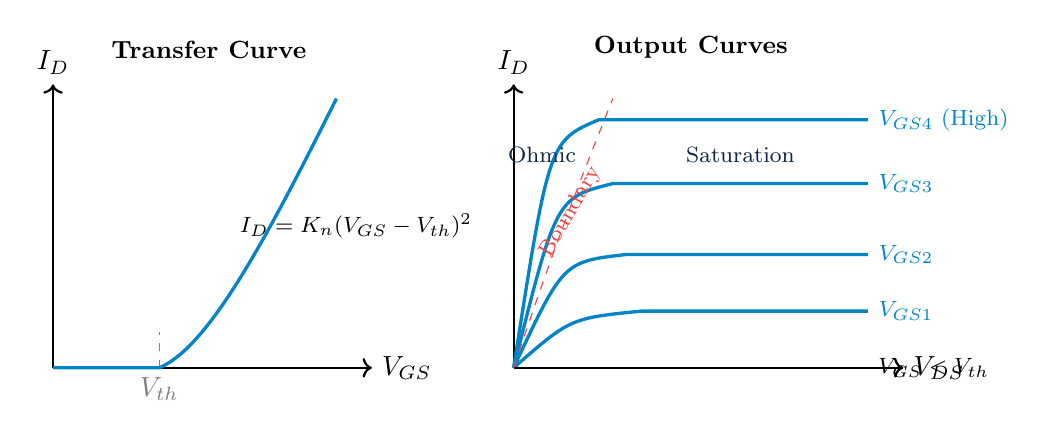
\begin{tikzpicture}[scale=0.9]
  % Transfer Characteristics
  \begin{scope}[xshift=0cm]
    \draw[thick,->] (0,0) -- (4.5,0) node[right] {$V_{GS}$};
    \draw[thick,->] (0,0) -- (0,4.0) node[above] {$I_D$};
    \draw[dashed,gray] (1.5,0) node[below] {$V_{th}$} -- (1.5,0.5);
    \draw[very thick,accentblue] (0,0) -- (1.5,0) .. controls (2.2,0.3) and (3.0,1.8) .. (4.0,3.8);
    \node[above=0.2cm,font=\small\bfseries] at (2.2,4.0) {Transfer Curve};
    \node[right,font=\footnotesize] at (2.5,2.0) {$I_D = K_n (V_{GS} - V_{th})^2$};
  \end{scope}
  
  % Output Characteristics
  \begin{scope}[xshift=6.5cm]
    \draw[thick,->] (0,0) -- (5.5,0) node[right] {$V_{DS}$};
    \draw[thick,->] (0,0) -- (0,4.0) node[above] {$I_D$};
    
    % Curves for various V_GS
    \draw[very thick,accentblue] (0,0) .. controls (0.5,3.2) .. (1.2,3.5) -- (5.0,3.5) node[right,font=\footnotesize] {$V_{GS4}$ (High)};
    \draw[very thick,accentblue] (0,0) .. controls (0.6,2.4) .. (1.4,2.6) -- (5.0,2.6) node[right,font=\footnotesize] {$V_{GS3}$};
    \draw[very thick,accentblue] (0,0) .. controls (0.7,1.5) .. (1.6,1.6) -- (5.0,1.6) node[right,font=\footnotesize] {$V_{GS2}$};
    \draw[very thick,accentblue] (0,0) .. controls (0.8,0.7) .. (1.8,0.8) -- (5.0,0.8) node[right,font=\footnotesize] {$V_{GS1}$};
    \draw[thick] (0,0) -- (5.0,0) node[right,font=\footnotesize] {$V_{GS} < V_{th}$};
    
    % Boundary between Ohmic and Saturation
    \draw[dashed,alertframe] (0,0) .. controls (0.6,1.8) and (1.0,2.8) .. (1.4,3.8);
    \node[alertframe,font=\footnotesize,rotate=60] at (0.8,2.2) {Boundary};
    \node[font=\footnotesize,navyprimary] at (0.4,3.0) {Ohmic};
    \node[font=\footnotesize,navyprimary] at (3.2,3.0) {Saturation};
    \node[above=0.2cm,font=\small\bfseries] at (2.5,4.0) {Output Curves};
  \end{scope}
\end{tikzpicture}
\caption{Transfer characteristics ($I_D$ vs. $V_{GS}$) and output characteristics ($I_D$ vs. $V_{DS}$) of a power MOSFET.}
\label{fig:mosfet_curves}
\end{figure}

In the on-state (fully switched ON in the Ohmic/Linear region), the total drain-to-source resistance $R_{DS(on)}$ is the series sum of internal physical components:
\begin{equation}
R_{DS(on)} = R_{\text{source}} + R_{ch} + R_{acc} + R_D + R_{sub}
\end{equation}
\begin{itemize}[leftmargin=*]
  \item $R_{ch}$: Inversion channel resistance, inversely proportional to $(V_{GS} - V_{th})$.
  \item $R_D$: \textbf{Drift region resistance}. For high-voltage silicon MOSFETs ($V_{BR} > 200\text{ V}$), $R_D$ dominates completely:
  \begin{equation}
  R_D \propto \frac{W_d}{N_d} \propto V_{BR}^{2.5}
  \end{equation}
  This $V_{BR}^{2.5}$ exponent represents the \textbf{Silicon Unipolar Limit}: Doubling the breakdown voltage rating increases $R_{DS(on)}$ by nearly $6\times$! Consequently, high-voltage silicon MOSFETs ($> 600\text{ V}$) have excessively high conduction loss, which led to the development of the IGBT.
\end{itemize}

\begin{conceptbox}[Positive Temperature Coefficient: Safe Paralleling]
The on-state resistance $R_{DS(on)}$ of a power MOSFET has a \textbf{positive temperature coefficient}:
\begin{equation}
\frac{dR_{DS(on)}}{dT_j} > 0
\end{equation}
As junction temperature rises, increased lattice vibrations (acoustic phonon scattering) decrease electron mobility $\mu_n$, causing $R_{DS(on)}$ to increase (typically doubling between $25^\circ\text{C}$ and $150^\circ\text{C}$).
\begin{itemize}
  \item When MOSFETs are connected in parallel, if one device runs hotter, its $R_{DS(on)}$ increases, which automatically sheds current to cooler parallel devices.
  \item This \textbf{self-balancing current sharing} prevents thermal runaway, making MOSFETs trivially easy to parallel without external ballast resistors.
\end{itemize}
\end{conceptbox}

\begin{figure}[htbp]
\centering
\includegraphics[width=0.65\textwidth]{mohan_thermal_chain.png}
\caption{Equivalent thermal circuit models: (a) transient thermal impedance $Z_{th}(t)$ using Foster RC ladder network; (b) complete steady-state and transient thermal model from junction to ambient. (Source: Mohan, Fig.\ 29-3)}
\end{figure}

\subsubsection{Dynamic Switching Dynamics \& The Miller Plateau}
Power MOSFET switching speed is governed by the charging and discharging of internal inter-electrode parasitic capacitances:
\begin{itemize}[leftmargin=*]
  \item $C_{gs}$ (Gate-to-Source capacitance): Constant, governed by gate oxide area.
  \item $C_{gd}$ (Gate-to-Drain / Miller capacitance): Highly non-linear; increases by up to $100\times$ as $V_{DS}$ drops near zero.
  \item $C_{ds}$ (Drain-to-Source capacitance): Voltage-dependent junction depletion capacitance.
\end{itemize}
Datasheets specify: $C_{iss} = C_{gs} + C_{gd}$, $C_{oss} = C_{ds} + C_{gd}$, $C_{rss} = C_{gd}$.

\begin{figure}[htbp]
\centering
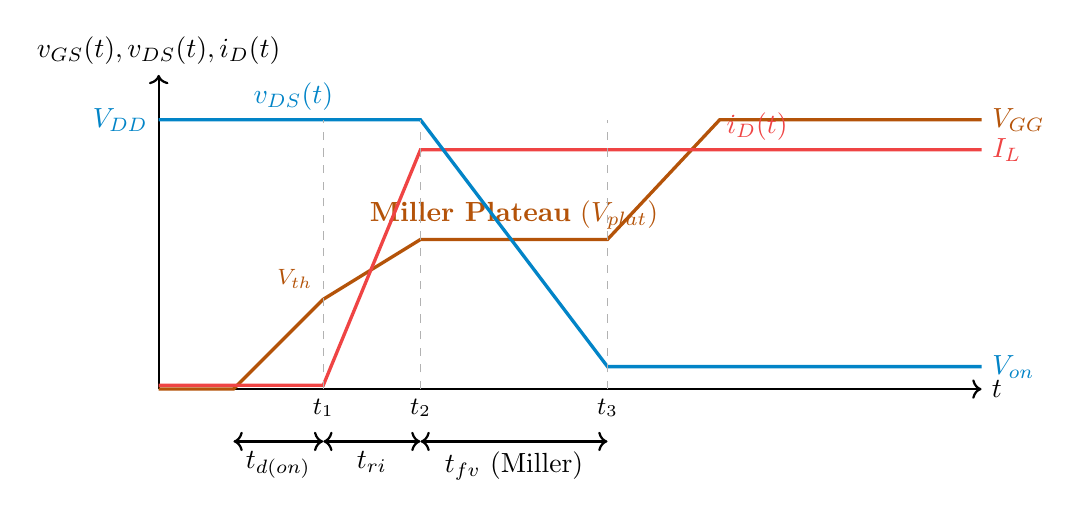
\begin{tikzpicture}[scale=0.95]
  % Axes
  \draw[thick,->] (0,0) -- (11.0,0) node[right] {$t$};
  \draw[thick,->] (0,0) -- (0,4.2) node[above] {$v_{GS}(t), v_{DS}(t), i_D(t)$};
  
  % Gate Voltage (gold)
  \draw[very thick,highlightgold] (0,0) -- (1.0,0) -- (2.2,1.2) node[above left,font=\footnotesize] {$V_{th}$} -- (3.5,2.0) -- (6.0,2.0) -- (7.5,3.6) -- (11,3.6) node[right] {$V_{GG}$};
  \node[highlightgold,above] at (4.75,2.0) {\textbf{Miller Plateau} ($V_{plat}$)};
  
  % Drain Current (red)
  \draw[very thick,alertframe] (0,0.05) -- (2.2,0.05) -- (3.5,3.2) -- (11,3.2) node[right] {$I_L$};
  \node[alertframe,above] at (8.0,3.2) {$i_D(t)$};
  
  % Drain Voltage (blue)
  \draw[very thick,accentblue] (0,3.6) node[left] {$V_{DD}$} -- (3.5,3.6) -- (6.0,0.3) -- (11,0.3) node[right] {$V_{on}$};
  \node[accentblue,above] at (1.8,3.6) {$v_{DS}(t)$};
  
  % Time markers
  \draw[dashed,gray!60] (2.2,0) -- (2.2,3.6);
  \node[below,text=black,font=\small\bfseries] at (2.2,0) {$t_1$};
  \draw[dashed,gray!60] (3.5,0) -- (3.5,3.6);
  \node[below,text=black,font=\small\bfseries] at (3.5,0) {$t_2$};
  \draw[dashed,gray!60] (6.0,0) -- (6.0,3.6);
  \node[below,text=black,font=\small\bfseries] at (6.0,0) {$t_3$};
  
  % Intervals
  \draw[<->,thick] (1.0,-0.7) -- (2.2,-0.7) node[midway,below] {$t_{d(on)}$};
  \draw[<->,thick] (2.2,-0.7) -- (3.5,-0.7) node[midway,below] {$t_{ri}$};
  \draw[<->,thick] (3.5,-0.7) -- (6.0,-0.7) node[midway,below] {$t_{fv}$ (Miller)};
\end{tikzpicture}
\caption{MOSFET turn-on switching dynamics illustrating the Miller Plateau during the drain voltage transition.}
\label{fig:mosfet_miller}
\end{figure}

\begin{conceptbox}[Physics of the Miller Plateau]
During turn-on with a clamped inductive load:
\begin{enumerate}
  \item \textbf{Interval $t_0 \to t_1$ (Turn-on Delay $t_{d(on)}$):} Gate current charges $C_{gs}$ from $0$ up to threshold voltage $V_{th}$. Drain current remains zero.
  \item \textbf{Interval $t_1 \to t_2$ (Current Rise $t_{ri}$):} $V_{GS}$ rises from $V_{th}$ to the Miller plateau level $V_{plat} = V_{th} + I_L / g_m$. Drain current rises from $0$ to full load current $I_L$.
  \item \textbf{Interval $t_2 \to t_3$ (Voltage Fall $t_{fv}$ --- The Miller Plateau):} 
    Once $i_D$ reaches $I_L$, the freewheeling diode turns off, allowing $v_{DS}$ to fall from $V_{DD}$ toward zero. 
    As $v_{DS}$ plunges, the rapidly changing voltage across the drain-to-gate capacitance draws a displacement current:
    \begin{equation}
    i_{gd} = C_{gd} \cdot \left|\frac{dv_{DS}}{dt}\right|
    \end{equation}
    \textbf{All gate driver current is diverted into discharging $C_{gd}$!} Zero current is left to charge $C_{gs}$. Consequently, \textbf{the gate-to-source voltage $V_{GS}$ remains completely flat} at the plateau voltage $V_{plat}$ until $v_{DS}$ finishes collapsing.
  \item \textbf{Interval $t_3 \to t_4$:} $V_{GS}$ resumes exponential charging toward the driver supply rail $V_{GG}$, driving the channel into deep ohmic conduction to minimize $R_{DS(on)}$.
\end{enumerate}
\end{conceptbox}

\subsection{Insulated Gate Bipolar Transistors (IGBTs)}

The \textbf{IGBT} is a three-terminal, voltage-controlled minority-carrier (bipolar) power semiconductor switch. It was invented by B. Jayant Baliga to combine the \textbf{high input impedance and fast MOS gate control} of a Power MOSFET with the \textbf{massive current-carrying capacity and low forward voltage drop} of a bipolar transistor.

\subsubsection{Physical Structure \& Working Principle}
The physical structure of an n-channel IGBT is identical to a vertical DMOSFET, with one revolutionary modification: \textbf{the $n^+$ drain substrate of the MOSFET is replaced by a heavily doped $p^+$ collector substrate!}

\begin{figure}[htbp]
\centering
\includegraphics[width=0.72\textwidth]{mohan_igbt_xsection.png}
\caption{Cross-sectional physical structure of an IGBT cell showing the $p^+$ collector injector substrate, $n^+$ buffer layer, $n^-$ drift base, and the internal MOS gate channel alongside carrier flow. (Source: Ned Mohan, Fig.\ 25-3)}
\label{fig:igbt_structure}
\end{figure}

\begin{enumerate}[leftmargin=*]
  \item \textbf{Four-Layer Architecture:} Forms a $p^+-n^--p-n^+$ sandwich (resembling a thyristor, but controlled by a MOS gate).
  \item \textbf{Conductivity Modulation in the Drift Layer:} When $V_{GE} > V_{GE(th)}$, the MOS gate induces an n-channel. Electrons flow from the $n^+$ emitter through the channel into the $n^-$ drift region.
  \item This electron current acts as the base current for the wide-base PNP transistor formed by $p^+$ (collector) / $n^-$ (drift base) / $p$ (emitter body).
  \item The $p^+$ substrate injects an immense swarm of \textbf{minority carrier holes} into the $n^-$ drift region.
  \item This floods the thick drift layer with an electron-hole plasma, causing massive \textbf{conductivity modulation}. The on-state voltage drop across the drift region collapses! A $1200\text{ V}, 100\text{ A}$ IGBT exhibits an on-state saturation voltage of merely:
  \begin{equation}
  V_{CE(sat)} \approx 1.5 - 2.0\text{ V}
  \end{equation}
  compared to $> 15\text{ V}$ for an equivalent silicon MOSFET!
\end{enumerate}

\subsubsection{Equivalent Circuit \& Parasitic Thyristor Latch-Up}

\begin{figure}[htbp]
\centering
\includegraphics[width=0.75\textwidth]{mohan_igbt_circuit.png}
\caption{Equivalent circuit models of the IGBT: (a) approximate equivalent circuit valid under normal operation (MOSFET driving a wide-base PNP bipolar transistor); (b) complete equivalent circuit showing the internal parasitic NPN transistor and the thyristor latch-up loop across $R_{\text{body}}$. (Source: Ned Mohan, Fig.\ 25-4)}
\label{fig:igbt_equivalent}
\end{figure}

\begin{alertbox}[The Danger of IGBT Latch-Up]
The 4-layer structure contains a parasitic NPN transistor ($Q_2$) that pairs with $Q_1$ to form an \textbf{unwanted internal SCR}:
\begin{itemize}
  \item The holes injected by $Q_1$ must travel laterally through the $p$-body to reach the emitter metallization.
  \item This lateral hole flow creates an ohmic voltage drop across the $p$-body resistance:
  \begin{equation}
  V_{BE2} = I_{\text{hole}} \cdot R_{\text{body}}
  \end{equation}
  \item If $V_{BE2} \ge 0.7\text{ V}$, the parasitic NPN transistor turns on, triggering \textbf{regenerative thyristor latch-up}!
  \item Once latched, the gate completely loses the ability to turn off collector current. The device suffers instantaneous short-circuit destruction.
\end{itemize}
\textbf{Modern Mitigation:} Modern Non-Punch-Through (NPT) and Field-Stop (FS) IGBTs employ heavily doped $p^+$ contact wells directly beneath the cathode to slash $R_{\text{body}}$ to near zero, raising the dynamic latch-up threshold to several times rated surge current.
\end{alertbox}

\subsubsection{Dynamic Switching Characteristics \& The Current Tail}
While the IGBT turns ON quickly like a MOSFET, its \textbf{turn-off behavior is strictly limited by bipolar physics}.

\begin{figure}[htbp]
\centering
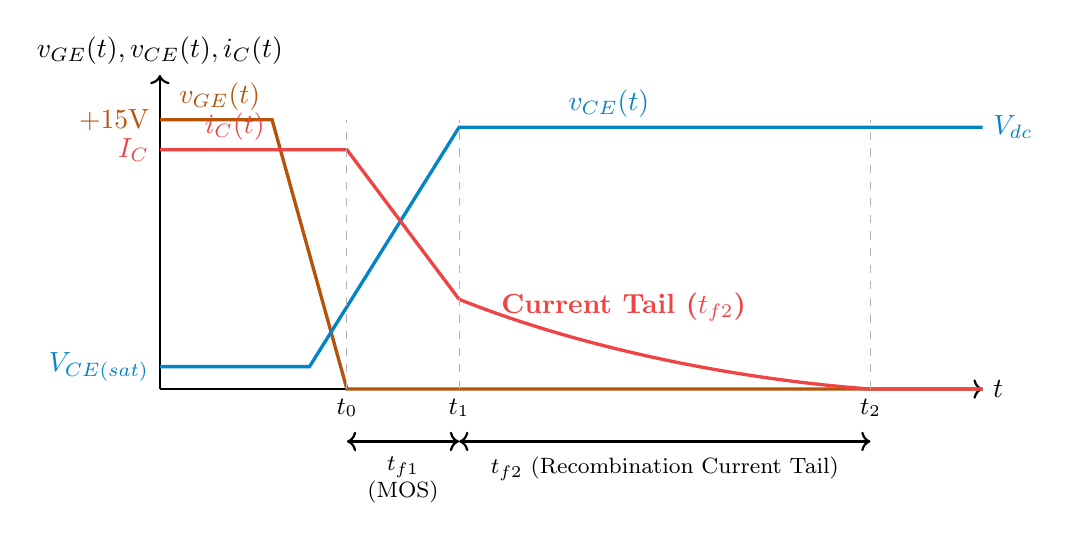
\begin{tikzpicture}[scale=0.95]
  % Axes
  \draw[thick,->] (0,0) -- (11.0,0) node[right] {$t$};
  \draw[thick,->] (0,0) -- (0,4.2) node[above] {$v_{GE}(t), v_{CE}(t), i_C(t)$};
  
  % Gate Voltage (gold)
  \draw[very thick,highlightgold] (0,3.6) node[left] {$+15\text{V}$} -- (1.5,3.6) -- (2.5,0) -- (11,0);
  \node[highlightgold,above] at (0.8,3.6) {$v_{GE}(t)$};
  
  % Collector Voltage (blue)
  \draw[very thick,accentblue] (0,0.3) node[left] {$V_{CE(sat)}$} -- (2.0,0.3) -- (4.0,3.5) -- (11,3.5) node[right] {$V_{dc}$};
  \node[accentblue,above] at (6.0,3.5) {$v_{CE}(t)$};
  
  % Collector Current (red) showing tailing
  \draw[very thick,alertframe] (0,3.2) node[left] {$I_C$} -- (2.5,3.2) -- (4.0,1.2);
  \draw[very thick,alertframe] (4.0,1.2) .. controls (5.5,0.6) and (7.5,0.15) .. (9.5,0) -- (11,0);
  \node[alertframe,above] at (1.0,3.2) {$i_C(t)$};
  \node[alertframe,font=\bfseries] at (6.2,1.1) {Current Tail ($t_{f2}$)};
  
  % Markers
  \draw[dashed,gray!60] (2.5,0) -- (2.5,3.6);
  \node[below,text=black,font=\small\bfseries] at (2.5,0) {$t_0$};
  \draw[dashed,gray!60] (4.0,0) -- (4.0,3.6);
  \node[below,text=black,font=\small\bfseries] at (4.0,0) {$t_1$};
  \draw[dashed,gray!60] (9.5,0) -- (9.5,3.6);
  \node[below,text=black,font=\small\bfseries] at (9.5,0) {$t_2$};
  
  % Intervals
  \draw[<->,thick] (2.5,-0.7) -- (4.0,-0.7) node[midway,below=2pt,align=center,font=\footnotesize] {$t_{f1}$\\(MOS)};
  \draw[<->,thick] (4.0,-0.7) -- (9.5,-0.7) node[midway,below=2pt,font=\footnotesize] {$t_{f2}$ (Recombination Current Tail)};
\end{tikzpicture}
\caption{IGBT turn-off switching waveforms highlighting the persistent collector current tailing effect.}
\label{fig:igbt_tail}
\end{figure}

\begin{conceptbox}[Physics of the Current Tail]
When gate-to-emitter voltage $v_{GE}$ is dropped below threshold:
\begin{enumerate}
  \item \textbf{Rapid Current Drop ($t_{f1}$):} The MOS channel collapses instantaneously, extinguishing the electron current component ($I_{MOS} \approx 60\% - 70\%$ of total $I_C$).
  \item \textbf{The Persistent Tail ($t_{f2}$):} 
    With the MOS channel closed, the base of the wide-base PNP bipolar transistor is now \textbf{open-circuited}!
    The massive store of excess minority holes trapped in the thick $n^-$ drift region has no external terminal through which to exit.
    These trapped carriers can disappear \textbf{only by natural recombination} ($\Delta p(t) = \Delta p_0 e^{-t/\tau_p}$).
  \item \textbf{Thermal Impact:} Because $v_{CE}$ has already risen to the full DC rail voltage $V_{dc}$ while this tail current persists, the instantaneous power dissipation $v_{CE}(t) \cdot i_C(t)$ during $t_{f2}$ is massive!
  \item \textbf{Frequency Limit:} The current tail drastically inflates the turn-off switching energy loss ($E_{off}$), restricting standard silicon IGBT switching frequencies to $\le 20 - 30\text{ kHz}$.
\end{enumerate}
\end{conceptbox}

\subsection{Gate Drive Circuits for MOSFETs and IGBTs}

Because power MOSFETs and IGBTs have insulated gates, their steady-state DC input resistance is $> 10^{10}\,\Omega$. However, dynamically, the gate represents a significant capacitive load ($C_{iss} \sim 1 - 10\text{ nF}$). To switch within tens of nanoseconds, the gate driver must source and sink high instantaneous peak currents:
\begin{equation}
I_{G,\text{peak}} = \frac{V_{GG} - V_{EE}}{R_G + R_{\text{int}}}
\end{equation}
where $R_G$ is the external series gate resistor and $R_{\text{int}}$ is the internal polysilicon gate resistance.

\subsubsection{Totem-Pole Push-Pull Driver}
The fundamental discrete gate driver is the complementary BJT totem-pole emitter-follower circuit:

\begin{figure}[htbp]
\centering
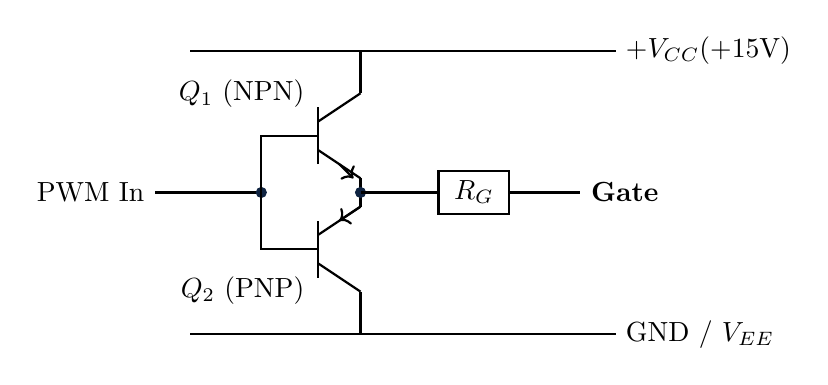
\begin{tikzpicture}[scale=0.9]
  % Rails
  \draw[thick] (0,4.0) -- (6,4.0) node[right] {$+V_{CC} (+15\text{V})$};
  \draw[thick] (0,0) -- (6,0) node[right] {GND / $V_{EE}$};
  
  % Input
  \draw[very thick] (-0.5,2.0) node[left] {PWM In} -- (1.0,2.0);
  \filldraw[navyprimary] (1.0,2.0) circle (2pt);
  
  % NPN Upper Transistor Q1
  \draw[thick] (1.0,2.0) -- (1.0,2.8) -- (1.8,2.8);
  \draw[thick] (1.8,2.4) -- (1.8,3.2); % Base
  \draw[thick] (1.8,3.0) -- (2.4,3.4); % Collector
  \draw[thick] (2.4,3.4) -- (2.4,4.0);
  \draw[thick] (1.8,2.6) -- (2.4,2.2); % Emitter
  \draw[thick,->] (2.1,2.4) -- (2.3,2.2);
  \node[above left=2pt] at (1.8,3.0) {$Q_1$ (NPN)};
  
  % PNP Lower Transistor Q2
  \draw[thick] (1.0,2.0) -- (1.0,1.2) -- (1.8,1.2);
  \draw[thick] (1.8,0.8) -- (1.8,1.6); % Base
  \draw[thick] (1.8,1.0) -- (2.4,0.6); % Collector
  \draw[thick] (2.4,0.6) -- (2.4,0);
  \draw[thick] (1.8,1.4) -- (2.4,1.8); % Emitter
  \draw[thick,->] (2.4,1.8) -- (2.1,1.6);
  \node[below left=2pt] at (1.8,1.0) {$Q_2$ (PNP)};
  
  % Node between emitters
  \draw[thick] (2.4,2.2) -- (2.4,1.8);
  \filldraw[navyprimary] (2.4,2.0) circle (2pt);
  \draw[thick] (2.4,2.0) -- (3.5,2.0);
  
  % Series Gate Resistor RG
  \draw[thick] (3.5,1.7) rectangle (4.5,2.3) node[midway] {$R_G$};
  \draw[very thick] (4.5,2.0) -- (5.5,2.0) node[right,font=\bfseries] {Gate};
\end{tikzpicture}
\caption{Totem-pole complementary push-pull gate driver providing high sourcing and sinking current capabilities.}
\label{fig:totem_pole}
\end{figure}

\begin{itemize}[leftmargin=*]
  \item When PWM input is HIGH, $Q_1$ (NPN) conducts, rapidly charging the gate to $+V_{CC}$ with peak current limited only by $R_G$.
  \item When PWM input is LOW, $Q_2$ (PNP) conducts, rapidly dumping the gate charge to ground ($V_{EE}$).
\end{itemize}

\subsubsection{Bootstrap Gate Driver Circuit (IR2110 Architecture)}
In half-bridge and full-bridge inverters, the source/emitter of the \textbf{high-side switch} is tied to the switching phase node ($V_S$), which swings violently between $0\text{ V}$ and the high-voltage DC bus ($V_{DC}$). Driving the high-side switch requires a floating gate voltage referenced to $V_S$.

The \textbf{bootstrap circuit} generates this floating supply without an expensive isolated DC-DC converter.

\begin{figure}[htbp]
\centering
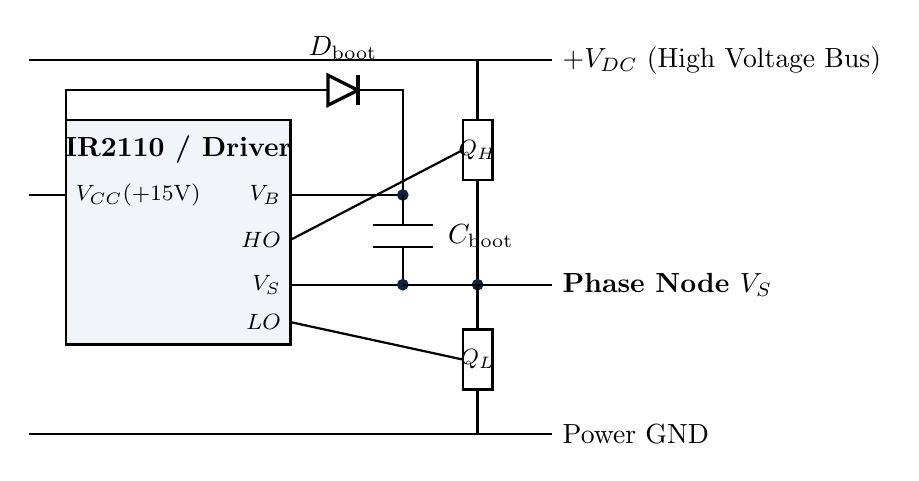
\begin{tikzpicture}[scale=0.95]
  % Rails
  \draw[thick] (0,5.0) -- (7,5.0) node[right] {$+V_{DC}$ (High Voltage Bus)};
  \draw[thick] (0,0) -- (7,0) node[right] {Power GND};
  
  % Driver IC block
  \draw[thick,fill=calloutbg] (0.5,1.2) rectangle (3.5,4.2);
  \node[font=\bfseries] at (2.0,3.8) {IR2110 / Driver};
  
  % Pins
  \node[right,font=\footnotesize] at (0.5,3.2) {$V_{CC} (+15\text{V})$};
  \node[left,font=\footnotesize] at (3.5,3.2) {$V_B$};
  \node[left,font=\footnotesize] at (3.5,2.6) {$HO$};
  \node[left,font=\footnotesize] at (3.5,2.0) {$V_S$};
  \node[left,font=\footnotesize] at (3.5,1.5) {$LO$};
  
  % Bootstrap diode D_boot
  \draw[thick] (0,3.2) -- (0.5,3.2);
  \draw[thick] (0.5,3.2) -- (0.5,4.6) -- (4.0,4.6);
  \draw[very thick,fill=white] (4.0,4.4) -- (4.4,4.6) -- (4.0,4.8) -- cycle;
  \draw[very thick] (4.4,4.4) -- (4.4,4.8);
  \node[above=2pt] at (4.2,4.8) {$D_{\text{boot}}$};
  \draw[thick] (4.4,4.6) -- (5.0,4.6) -- (5.0,3.2) -- (3.5,3.2);
  
  % Bootstrap capacitor C_boot
  \filldraw[navyprimary] (5.0,3.2) circle (2pt);
  \draw[thick] (5.0,3.2) -- (5.0,2.8);
  \draw[thick] (4.6,2.8) -- (5.4,2.8);
  \draw[thick] (4.6,2.5) -- (5.4,2.5);
  \node[right=2pt] at (5.4,2.65) {$C_{\text{boot}}$};
  \draw[thick] (5.0,2.5) -- (5.0,2.0) -- (3.5,2.0);
  
  % High side switch
  \filldraw[navyprimary] (5.0,2.0) circle (2pt);
  \draw[thick] (6.0,5.0) -- (6.0,4.2); % Drain
  \draw[thick] (5.8,3.4) rectangle (6.2,4.2) node[midway,font=\footnotesize] {$Q_H$};
  \draw[thick] (6.0,3.4) -- (6.0,2.0); % Source / Phase node
  \draw[thick] (3.5,2.6) -- (5.8,3.8); % Gate drive
  
  % Phase node connection
  \filldraw[navyprimary] (6.0,2.0) circle (2pt);
  \draw[thick] (5.0,2.0) -- (6.0,2.0) -- (7.0,2.0) node[right,font=\bfseries] {Phase Node $V_S$};
  
  % Low side switch
  \draw[thick] (6.0,2.0) -- (6.0,1.4);
  \draw[thick] (5.8,0.6) rectangle (6.2,1.4) node[midway,font=\footnotesize] {$Q_L$};
  \draw[thick] (6.0,0.6) -- (6.0,0);
  \draw[thick] (3.5,1.5) -- (5.8,1.0); % LO drive
\end{tikzpicture}
\caption{Bootstrap gate drive topology (IR2110 architecture) supplying the floating high-side gate charge.}
\label{fig:bootstrap_driver}
\end{figure}

\begin{conceptbox}[Operating Principles of the Bootstrap Driver]
\begin{enumerate}[leftmargin=*]
  \item \textbf{Charging Phase (Low-Side Switch ON):} When $Q_L$ is turned ON, the phase node $V_S$ is pulled to ground ($0\text{ V}$). Fast diode $D_{\text{boot}}$ becomes forward-biased, charging bootstrap capacitor $C_{\text{boot}}$ from $V_{CC}$ ($+15\text{V}$) up to approximately $(V_{CC} - V_D)$.
  \item \textbf{Floating Phase (High-Side Switch ON):} When $Q_L$ turns OFF and $Q_H$ turns ON, $V_S$ leaps up to the DC bus voltage $V_{DC}$. Diode $D_{\text{boot}}$ becomes reverse-biased, isolating the low-voltage supply. The capacitor $C_{\text{boot}}$ floats with $V_S$, providing a stable $(V_S + 15\text{V})$ rail between pins $V_B$ and $V_S$ to keep $Q_H$ fully enhanced.
  \item \textbf{Duty Cycle Limitation:} Because $C_{\text{boot}}$ can recharge \textbf{only when $Q_L$ is ON} ($V_S = 0$), a bootstrap circuit \textbf{cannot operate at $100\%$ duty cycle ($D < 1$)}. Periodic low-side conduction is strictly required.
\end{enumerate}
\end{conceptbox}

\begin{formulabox}[Bootstrap Capacitor Sizing Equation]
The capacitor $C_{\text{boot}}$ must supply the gate charge $Q_g$, the driver quiescent current $I_{QBS}$, level-shift charge $Q_{LS}$, and leakage currents during the maximum high-side on-time $t_{on,\max}$, while limiting the voltage drop across $C_{\text{boot}}$ to $\Delta V_{\text{boot}} \le 0.5 - 1.0\text{ V}$:
\begin{equation}
C_{\text{boot}} \ge \frac{Q_g + I_{QBS} \cdot t_{on,\max} + Q_{LS} + I_{\text{leak}} \cdot t_{on,\max}}{\Delta V_{\text{boot}}}
\end{equation}
A typical design rule of thumb selects $C_{\text{boot}} \ge 10 \text{ to } 15 \times C_{iss}$.
\end{formulabox}

%%%%%%%%%%%%%%%%%%%%%%%%%%%%%%%%%%%%%%%%%%%%%%%%%%%%%%%%%%%%%%%%%%%%%%%%%%%%%%%
\section{Modern Power Devices: Wide Bandgap (WBG) Semiconductors}
%%%%%%%%%%%%%%%%%%%%%%%%%%%%%%%%%%%%%%%%%%%%%%%%%%%%%%%%%%%%%%%%%%%%%%%%%%%%%%%

\subsection{Physical Limitations of Silicon}

For over six decades, Silicon (Si) has served as the bedrock of power semiconductor technology. However, silicon is rapidly approaching its fundamental, immutable physical limits imposed by its material properties:
\begin{enumerate}[leftmargin=*]
  \item \textbf{Narrow Bandgap ($E_g = 1.12\text{ eV}$):} Under high temperatures ($T_j > 150^\circ\text{C}$), thermal energy excites valence electrons across the narrow bandgap into the conduction band ($n_i \propto T^{3/2} e^{-E_g / 2 k T}$), causing excessive intrinsic leakage currents and thermal runaway.
  \item \textbf{Low Critical Breakdown Electric Field ($E_c \approx 0.3\text{ MV/cm}$):} Silicon can withstand an electric field of only $30\text{ V}/\mu\text{m}$ before avalanche impact ionization occurs. To block thousands of volts, the $n^-$ drift region must be made extraordinarily thick and lightly doped ($W_d \propto V_{BR}, N_d \propto 1/V_{BR}^2$).
  \item \textbf{The Silicon Unipolar Limit:}
    According to Baliga's Figure of Merit (BFOM), the minimum theoretical specific on-resistance of a unipolar drift region is:
    \begin{equation}
    R_{on,sp} = \frac{4 V_{BR}^2}{\epsilon_s \cdot \mu_n \cdot E_c^3}
    \end{equation}
    Because $E_c$ is low for silicon, $R_{on,sp}$ scales aggressively with $V_{BR}^2$. For ratings above $600\text{ V}$, silicon MOSFETs become prohibitively resistive, forcing the use of bipolar devices (IGBTs) with their inherent switching frequency limitations (current tailing).
  \item \textbf{Moderate Thermal Conductivity ($k = 1.5\text{ W/cm}\cdot\text{K}$):} Silicon cannot evacuate heat rapidly, requiring large, heavy heat sinks and forced liquid cooling systems.
\end{enumerate}

\subsection{Wide Bandgap Semiconductors: SiC and GaN}

\textbf{Wide Bandgap (WBG)} semiconductors—principally \textbf{Silicon Carbide (4H-SiC)} and \textbf{Gallium Nitride (GaN)}—possess electronic bandgaps approximately three times wider than silicon.

\begin{table}[htbp]
\centering
\small
\caption{Fundamental Material Properties: Silicon (Si) vs. 4H-SiC vs. Gallium Nitride (GaN)}
\label{tab:wbg_properties}
\begin{tabularx}{\textwidth}{l Y Y Y}
\toprule
\textbf{Physical Property} & \textbf{Silicon (Si)} & \textbf{Silicon Carbide (4H-SiC)} & \textbf{Gallium Nitride (GaN)} \\
\midrule
\textbf{Bandgap Energy ($E_g$)} & $1.12\text{ eV}$ & $3.26\text{ eV}$ ($2.9\times$) & $3.40\text{ eV}$ ($3.0\times$) \\
\textbf{Critical Breakdown Field ($E_c$)} & $0.3\text{ MV/cm}$ & $2.8\text{ MV/cm}$ ($9.3\times$) & $3.3\text{ MV/cm}$ ($11.0\times$) \\
\textbf{Electron Mobility ($\mu_n$)} & $1400\text{ cm}^2/\text{V}\cdot\text{s}$ & $900\text{ cm}^2/\text{V}\cdot\text{s}$ & $1500 - 2000\text{ cm}^2/\text{V}\cdot\text{s}$ (2DEG) \\
\textbf{Saturated Electron Velocity ($v_{sat}$)} & $1.0 \times 10^7\text{ cm/s}$ & $2.0 \times 10^7\text{ cm/s}$ ($2.0\times$) & $2.5 \times 10^7\text{ cm/s}$ ($2.5\times$) \\
\textbf{Thermal Conductivity ($k$)} & $1.5\text{ W/cm}\cdot\text{K}$ & $4.9\text{ W/cm}\cdot\text{K}$ ($3.3\times$) & $1.5 - 2.0\text{ W/cm}\cdot\text{K}$ \\
\textbf{Dielectric Constant ($\epsilon_r$)} & $11.8$ & $9.7$ & $8.9$ \\
\textbf{Max Operating Temp ($T_{j,\max}$)} & $150^\circ\text{C}$ & $> 200^\circ\text{C} - 250^\circ\text{C}$ & $> 200^\circ\text{C}$ \\
\textbf{Baliga's FOM ($\propto \epsilon \mu E_c^3$)} & $1.0$ (Baseline) & $\approx 500$ & $\approx 1000 - 1500$ \\
\bottomrule
\end{tabularx}
\end{table}

\begin{conceptbox}[The Revolutionary Impact of a $10\times$ Higher Breakdown Field ($E_c$)]
The breakdown electric field $E_c$ enters the unipolar specific on-resistance equation to the \textbf{third power} ($E_c^3$):
\begin{equation}
R_{on,sp} \propto \frac{1}{E_c^3}
\end{equation}
Because SiC and GaN exhibit $E_c$ values roughly $10\times$ greater than silicon:
\begin{enumerate}
  \item \textbf{$10\times$ Thinner Drift Layer ($W_d \propto V_{BR} / E_c$):} A $1200\text{ V}$ SiC drift layer requires only $\sim 10\,\mu\text{m}$ of thickness, compared to $\sim 100\,\mu\text{m}$ in silicon.
  \item \textbf{$100\times$ Higher Doping Concentration ($N_d \propto E_c^2 / V_{BR}$):} The drift layer can be doped 100 times more heavily without premature breakdown.
  \item \textbf{Drastic Resistance Reduction:} Combining a $10\times$ thinner layer with $100\times$ higher conductivity reduces the theoretical drift resistance by up to \textbf{$1000\times$} compared to a silicon MOSFET!
  \item \textbf{Unipolar Operation at High Voltage:} High-voltage SiC MOSFETs ($1200\text{ V} - 3300\text{ V}$) can operate as pure unipolar majority-carrier switches, completely eliminating the minority carrier current tailing of IGBTs!
\end{enumerate}
\end{conceptbox}

\subsection{Silicon Carbide (SiC) MOSFETs}

Silicon Carbide (4H-SiC) is the premier material for high-power, high-voltage ($650\text{ V} - 3300\text{ V}+$) conversion:
\begin{itemize}[leftmargin=*]
  \item \textbf{Direct Replacement of Silicon IGBTs:} SiC MOSFETs replace $1200\text{ V}$ IGBTs in EV traction inverters, slashing total inverter power losses by $60\% - 75\%$ and extending EV driving range by $5\% - 10\%$ on the same battery capacity.
  \item \textbf{Superb Thermal Conductivity ($k = 4.9\text{ W/cm}\cdot\text{K}$):} SiC conducts heat three times better than silicon, enabling dramatic miniaturization of heat sinks.
  \item \textbf{Extremely Low Switching Losses:} Because SiC MOSFETs are unipolar, $E_{off}$ is dictated purely by capacitance discharge without any carrier recombination tail. Operating frequencies can be pushed from $15\text{ kHz}$ (IGBT) to $100\text{ kHz} - 300\text{ kHz}$.
  \item \textbf{Body Diode Nuance:} The wide bandgap gives the intrinsic SiC body diode a high forward knee voltage ($V_F \approx 3.2 - 4.0\text{ V}$). If current freewheels through the body diode during dead-time, conduction losses are high. Engineers solve this using \textbf{synchronous rectification} (turning on the SiC channel during reverse freewheeling) or adding an anti-parallel SiC Schottky barrier diode.
  \item \textbf{Gate Drive Levels:} Because SiC has a lower channel inversion layer mobility due to $\text{SiO}_2/\text{SiC}$ interface traps, a higher gate-to-source voltage ($+18\text{ V} \text{ to } +20\text{ V}$) is required to achieve minimal $R_{DS(on)}$. A negative turn-off bias ($-4\text{ V} \text{ to } -5\text{ V}$) is universally employed to prevent spurious Miller turn-on under extreme $dv/dt$ ($> 50\text{ V/ns}$).
\end{itemize}

\subsection{Gallium Nitride (GaN) HEMTs}

Gallium Nitride power devices are constructed as lateral \textbf{High Electron Mobility Transistors (HEMTs)}.

\subsubsection{Physics of the Two-Dimensional Electron Gas (2DEG)}
Unlike silicon MOSFETs that require gate voltage to invert the channel, the GaN HEMT features a spontaneous, ultra-conductive channel known as the \textbf{Two-Dimensional Electron Gas (2DEG)}:

\begin{figure}[htbp]
\centering
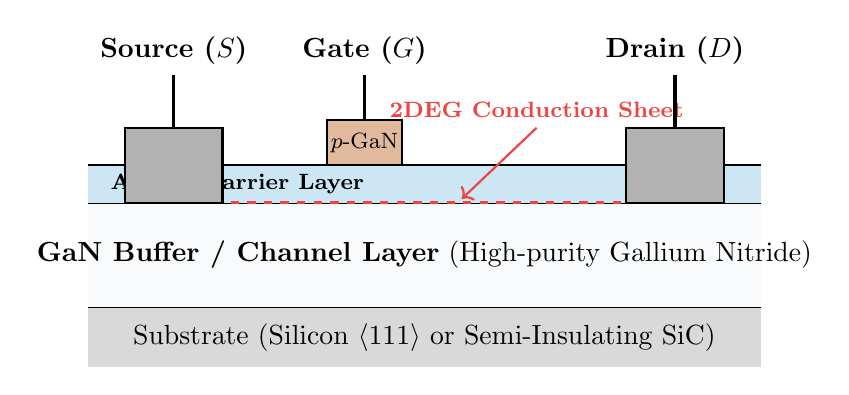
\begin{tikzpicture}[scale=0.95]
  % Substrate (Silicon or SiC)
  \fill[gray!30] (0,0) rectangle (9,0.8);
  \draw[thick] (0,0.8) -- (9,0.8);
  \node at (4.5,0.4) {Substrate (Silicon $\langle 111 \rangle$ or Semi-Insulating SiC)};
  
  % GaN buffer layer
  \fill[cardbg] (0,0.8) rectangle (9,2.2);
  \draw[thick] (0,2.2) -- (9,2.2);
  \node at (4.5,1.5) {\textbf{GaN Buffer / Channel Layer} (High-purity Gallium Nitride)};
  
  % AlGaN barrier layer
  \fill[accentblue!20] (0,2.2) rectangle (9,2.7);
  \draw[thick] (0,2.7) -- (9,2.7);
  \node[font=\footnotesize] at (2.0,2.45) {\textbf{AlGaN Barrier Layer}};
  
  % 2DEG Sheet at interface (red dashed line)
  \draw[very thick,alertframe,dashed] (0.8,2.2) -- (8.2,2.2);
  \draw[->,thick,alertframe] (6.0,3.2) node[above,font=\footnotesize\bfseries] {2DEG Conduction Sheet} -- (5.0,2.25);
  
  % Ohmic Source Contact
  \fill[gray!60] (0.5,2.2) rectangle (1.8,3.2);
  \draw[thick] (0.5,2.2) rectangle (1.8,3.2);
  \draw[very thick] (1.15,3.2) -- (1.15,3.9) node[above,font=\bfseries] {Source ($S$)};
  
  % Ohmic Drain Contact
  \fill[gray!60] (7.2,2.2) rectangle (8.5,3.2);
  \draw[thick] (7.2,2.2) rectangle (8.5,3.2);
  \draw[very thick] (7.85,3.2) -- (7.85,3.9) node[above,font=\bfseries] {Drain ($D$)};
  
  % Schottky / p-GaN Gate
  \fill[highlightgold!40] (3.2,2.7) rectangle (4.2,3.3);
  \draw[thick] (3.2,2.7) rectangle (4.2,3.3);
  \draw[very thick] (3.7,3.3) -- (3.7,3.9) node[above,font=\bfseries] {Gate ($G$)};
  \node[font=\footnotesize] at (3.7,3.0) {$p$-GaN};
\end{tikzpicture}
\caption{Heterojunction architecture of a lateral GaN High Electron Mobility Transistor (HEMT) showing the spontaneously formed 2DEG conduction sheet.}
\label{fig:gan_hemt}
\end{figure}

\begin{enumerate}[leftmargin=*]
  \item \textbf{Heterojunction Formation:} When a thin layer of Aluminum Gallium Nitride (AlGaN) is grown epitaxially on high-purity GaN, the difference in spontaneous polarization and the massive piezoelectric stress at the lattice-mismatched interface induce an intense internal electric field.
  \item \textbf{Carrier Confinement:} This field bends the conduction band below the Fermi level at the interface, trapping electrons in a quantum well just a few nanometers thick: the \textbf{2DEG}.
  \item \textbf{Phenomenal Mobility Without Doping:} 
    Unlike silicon or SiC where high conductivity requires intentional donor doping (which causes ionized impurity scattering), the 2DEG is populated purely by polarization charges! 
    Because the channel is free of dopant atoms, electrons glide through the crystal lattice with virtually zero scattering, achieving an extraordinary electron mobility:
    \begin{equation}
    \mu_{2DEG} \approx 1500 - 2000\text{ cm}^2/\text{V}\cdot\text{s}
    \end{equation}
  \item \textbf{Depletion-Mode (d-mode) vs. Enhancement-Mode (e-mode):}
    \begin{itemize}
      \item \textbf{d-mode (Normally-ON):} Because the 2DEG is formed naturally by crystal physics, a standard GaN HEMT conducts heavy current at $V_{GS} = 0\text{ V}$. In power electronics, normally-on switches present severe safety hazards during power-up.
      \item \textbf{p-GaN Gate e-mode (Normally-OFF):} Growing a heavily doped p-type GaN layer beneath the gate lifts the conduction band above the Fermi level, completely depleting the 2DEG directly under the gate at zero bias ($V_{th} \approx +1.4 - 1.7\text{ V}$). Applying $V_{GS} \ge 5\text{ V}$ re-establishes the 2DEG channel.
    \end{itemize}
\end{enumerate}

\subsubsection{The GaN Cascode Configuration}
Another widely adopted approach to achieve safe, normally-off operation is the \textbf{Cascode Configuration}:

\begin{figure}[htbp]
\centering
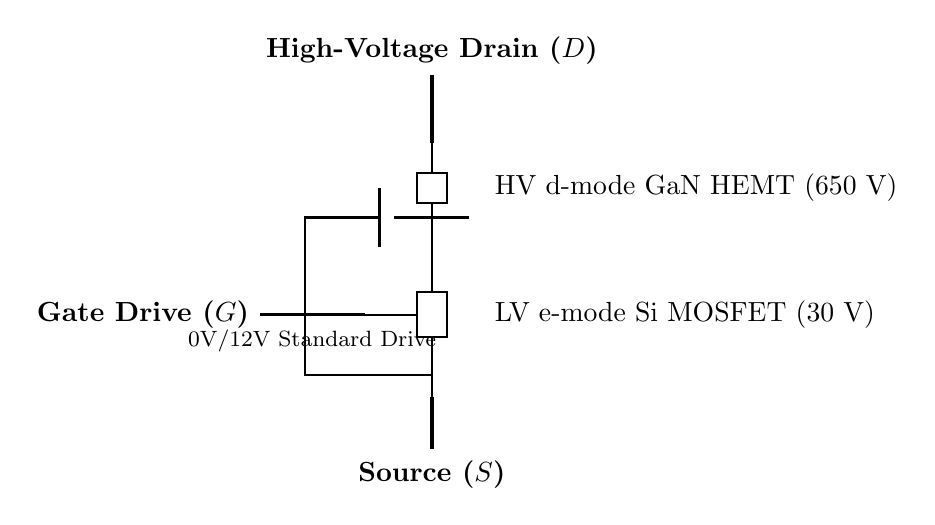
\begin{tikzpicture}[scale=0.95]
  % Rails / Terminals
  \draw[very thick] (2.5,4.5) node[above,font=\bfseries] {High-Voltage Drain ($D$)} -- (2.5,3.6);
  
  % GaN HEMT (Depletion Mode, high voltage)
  \draw[thick] (2.0,2.6) -- (3.0,2.6); % Drain to source
  \draw[thick] (2.5,3.6) -- (2.5,3.2); % Drain
  \draw[thick] (2.3,3.2) rectangle (2.7,2.8);
  \node[right=0.2cm] at (3.0,3.0) {HV d-mode GaN HEMT ($650\text{ V}$)};
  \draw[thick] (2.5,2.8) -- (2.5,2.0); % Source
  \draw[thick] (1.8,3.0) -- (1.8,2.2); % Gate
  
  % Connection GaN Gate to Low-Voltage MOSFET Source
  \draw[thick] (1.8,2.6) -- (0.8,2.6) -- (0.8,0.5) -- (2.5,0.5);
  
  % Low-Voltage Silicon MOSFET (Enhancement Mode)
  \draw[thick] (2.3,1.6) rectangle (2.7,1.0);
  \node[right=0.2cm] at (3.0,1.3) {LV e-mode Si MOSFET ($30\text{ V}$)};
  \draw[thick] (2.5,2.0) -- (2.5,1.6); % Drain
  \draw[thick] (2.5,1.0) -- (2.5,0.2); % Source
  \draw[very thick] (2.5,0.2) -- (2.5,-0.5) node[below,font=\bfseries] {Source ($S$)};
  
  % Gate terminal of Si MOSFET
  \draw[thick] (1.6,1.3) -- (2.3,1.3);
  \draw[very thick] (1.6,1.3) -- (0.2,1.3) node[left,font=\bfseries] {Gate Drive ($G$)};
  \node[below=2pt,font=\footnotesize] at (0.9,1.3) {$0\text{V} / 12\text{V}$ Standard Drive};
\end{tikzpicture}
\caption{GaN Cascode configuration pairing a low-voltage Silicon MOSFET with a high-voltage depletion-mode GaN HEMT.}
\label{fig:gan_cascode}
\end{figure}

\begin{conceptbox}[Operating Principle of the GaN Cascode]
\begin{enumerate}
  \item When Gate Drive $V_G = 0\text{ V}$, the low-voltage Si MOSFET is OFF. The phase current charges the parasitic capacitance between the two devices until the GaN source reaches $+20\text{ V}$ to $+30\text{ V}$.
  \item Because the GaN gate is tied to ground (the Si MOSFET source), the GaN gate-to-source voltage is $V_{GS,\text{GaN}} = -25\text{ V}$, which is well beyond its pinch-off voltage ($-10\text{ V}$). The high-voltage GaN HEMT shuts OFF completely, safely blocking the entire $650\text{ V}$ bus!
  \item When $V_G = 12\text{ V}$, the Si MOSFET turns ON hard, pulling the GaN source to ground ($V_{GS,\text{GaN}} \to 0\text{ V}$). The GaN HEMT immediately turns ON.
  \item \textbf{Huge Engineering Benefit:} The cascode uses standard, rugged Silicon gate driver ICs ($0-12\text{ V}$) and has high noise immunity, while delivering the ultra-fast switching speed and zero reverse recovery of GaN!
\end{enumerate}
\end{conceptbox}

\subsubsection{Key Features \& Advantages of GaN HEMTs}
\begin{itemize}[leftmargin=*]
  \item \textbf{True Zero Reverse Recovery ($Q_{rr} = 0$):} Because the 2DEG channel has \textbf{zero minority carrier storage}, there is no reverse recovery delay when reverse current ceases. The device freewheels in the third quadrant by channel conduction without reverse recovery loss!
  \item \textbf{Extreme Switching Frequencies ($500\text{ kHz} - 10\text{ MHz}$):} The input capacitance ($C_{iss}$) and output capacitance ($C_{oss}$) of a GaN HEMT are an order of magnitude smaller than a silicon MOSFET of identical current rating. This allows switching frequencies an order of magnitude higher with minimal power loss.
  \item \textbf{Radical Miniaturization of Magnetics:} Operating at megahertz frequencies shrinks the physical volume of inductors and transformers by $80\%$, enabling the pocket-sized USB-PD 65W–240W laptop chargers that have revolutionized consumer electronics.
\end{itemize}

%%%%%%%%%%%%%%%%%%%%%%%%%%%%%%%%%%%%%%%%%%%%%%%%%%%%%%%%%%%%%%%%%%%%%%%%%%%%%%%
\section{Solved Numerical Examination Problems}
%%%%%%%%%%%%%%%%%%%%%%%%%%%%%%%%%%%%%%%%%%%%%%%%%%%%%%%%%%%%%%%%%%%%%%%%%%%%%%%

This section presents nine fully worked, textbook-grade numerical problems spanning every quantitative concept in Module 1. Each problem provides the full problem statement, systematic identification of given data, rigorous step-by-step arithmetic, explicit unit conversions, and key engineering takeaways.

%------------------------------------------------------------------------------
\subsection{Problem 1: Thermal Modeling and Heat Sink Sizing}
%------------------------------------------------------------------------------

\begin{examplebox}[Problem 1: Thermal Resistance Network \& Heat Sink Selection]
A power MOSFET packaged in a standard TO-220 case operates in a DC-DC switching regulator and dissipates an average continuous power of $P_D = 28\text{ W}$. The maximum allowable junction temperature specified by the manufacturer is $T_{j,\max} = 150^\circ\text{C}$, and the ambient air temperature inside the converter enclosure is $T_a = 45^\circ\text{C}$.

The device datasheet provides the junction-to-case thermal resistance as $R_{\theta,jc} = 1.25^\circ\text{C/W}$. The transistor is mechanically clamped to an extruded aluminum heat sink using a thermal silicone pad and zinc oxide grease, yielding an interface case-to-sink thermal resistance of $R_{\theta,cs} = 0.35^\circ\text{C/W}$.

\textbf{Determine:}
\begin{enumerate}[label=(\alph*)]
  \item The maximum permissible thermal resistance of the heat sink to ambient ($R_{\theta,sa}$).
  \item The operating case temperature ($T_c$) and heat sink surface temperature ($T_s$) at rated load.
  \item The maximum power the MOSFET can safely dissipate if operated \textbf{without a heat sink} in still air, given that the case-to-ambient thermal resistance is $R_{\theta,ca} = 55^\circ\text{C/W}$.
\end{enumerate}

\tcblower
\textbf{Solution:}

\textbf{Step 1: Identify Given Data}
\begin{itemize}[leftmargin=*]
  \item Average power dissipation: $P_D = 28\text{ W}$
  \item Maximum permissible junction temperature: $T_{j,\max} = 150^\circ\text{C}$
  \item Ambient temperature: $T_a = 45^\circ\text{C}$
  \item Junction-to-case thermal resistance: $R_{\theta,jc} = 1.25^\circ\text{C/W}$
  \item Case-to-sink thermal resistance: $R_{\theta,cs} = 0.35^\circ\text{C/W}$
  \item Free-air case-to-ambient resistance: $R_{\theta,ca} = 55^\circ\text{C/W}$
\end{itemize}

\textbf{Step 2: Calculate Maximum Allowable Total Thermal Resistance ($R_{\theta,ja}$)}
Applying the steady-state thermal Ohm's law:
\begin{equation}
T_j - T_a = P_D \cdot R_{\theta,ja} \implies R_{\theta,ja} = \frac{T_{j,\max} - T_a}{P_D}
\end{equation}
Substituting numerical values:
\begin{equation}
R_{\theta,ja} = \frac{150^\circ\text{C} - 45^\circ\text{C}}{28\text{ W}} = \frac{105^\circ\text{C}}{28\text{ W}} = 3.75^\circ\text{C/W}
\end{equation}

\textbf{Step 3: Calculate Required Heat Sink Thermal Resistance ($R_{\theta,sa}$)}
The total series thermal resistance is:
\begin{equation}
R_{\theta,ja} = R_{\theta,jc} + R_{\theta,cs} + R_{\theta,sa}
\end{equation}
Rearranging to solve for $R_{\theta,sa}$:
\begin{equation}
R_{\theta,sa} \le R_{\theta,ja} - (R_{\theta,jc} + R_{\theta,cs})
\end{equation}
\begin{equation}
R_{\theta,sa} \le 3.75 - (1.25 + 0.35) = 3.75 - 1.60 = \mathbf{2.15^\circ\text{C/W}}
\end{equation}
\textit{Takeaway:} The design engineer must select an extruded aluminum heat sink with a thermal resistance rating of \textbf{$2.15^\circ\text{C/W}$ or lower}.

\textbf{Step 4: Calculate Operating Case and Sink Temperatures}
The case temperature is:
\begin{equation}
T_c = T_j - P_D \cdot R_{\theta,jc} = 150^\circ\text{C} - (28\text{ W} \times 1.25^\circ\text{C/W}) = 150 - 35 = \mathbf{115.0^\circ\text{C}}
\end{equation}
The heat sink temperature is:
\begin{equation}
T_s = T_c - P_D \cdot R_{\theta,cs} = 115.0^\circ\text{C} - (28\text{ W} \times 0.35^\circ\text{C/W}) = 115.0 - 9.8 = \mathbf{105.2^\circ\text{C}}
\end{equation}
Checking against ambient:
\begin{equation}
T_s = T_a + P_D \cdot R_{\theta,sa} = 45 + (28 \times 2.15) = 45 + 60.2 = 105.2^\circ\text{C} \quad (\text{Confirmed})
\end{equation}

\textbf{Step 5: Maximum Power Dissipation Without Heat Sink}
In free air without a heat sink:
\begin{equation}
R_{\theta,ja(\text{free air})} = R_{\theta,jc} + R_{\theta,ca} = 1.25 + 55 = 56.25^\circ\text{C/W}
\end{equation}
The maximum safe continuous power is:
\begin{equation}
P_{D,\max(\text{no sink})} = \frac{T_{j,\max} - T_a}{R_{\theta,ja(\text{free air})}} = \frac{150 - 45}{56.25} = \frac{105}{56.25} = \mathbf{1.867\text{ W}}
\end{equation}
\textit{Critical Insight:} Without a heat sink, dissipating just $1.87\text{ W}$ heats the silicon junction to its absolute destruction limit ($150^\circ\text{C}$). Sizing the heat sink correctly increases power capability by fifteen-fold!
\end{examplebox}

%------------------------------------------------------------------------------
\subsection{Problem 2: Power Diode Reverse Recovery Dynamics}
%------------------------------------------------------------------------------

\begin{examplebox}[Problem 2: Reverse Recovery Transient Calculations]
A fast recovery power diode conducts a forward DC current of $I_F = 80\text{ A}$. During converter turn-off, the circuit applies a reverse voltage $V_R = 450\text{ V}$, forcing the diode current to ramp down at a constant rate of $di/dt = 120\text{ A}/\mu\text{s} = 1.2 \times 10^8\text{ A/s}$.

The diode exhibits a total reverse recovery time of $t_{rr} = 2.5\,\mu\text{s}$ with a softness factor of $S = t_b / t_a = 0.25$.

\textbf{Calculate:}
\begin{enumerate}[label=(\alph*)]
  \item The storage interval ($t_a$) and fall/decay interval ($t_b$).
  \item The peak reverse recovery current ($I_{RR}$).
  \item The total reverse recovery stored charge ($Q_{RR}$).
  \item The reverse recovery power loss dissipated in the diode if operated at switching frequency $f_{sw} = 20\text{ kHz}$.
\end{enumerate}

\tcblower
\textbf{Solution:}

\textbf{Step 1: Calculate $t_a$ and $t_b$}
We are given:
\begin{equation}
t_{rr} = t_a + t_b = 2.5\,\mu\text{s}, \qquad S = \frac{t_b}{t_a} = 0.25 \implies t_b = 0.25 t_a
\end{equation}
Substituting $t_b$ into the total time equation:
\begin{equation}
t_a + 0.25 t_a = 1.25 t_a = 2.5\,\mu\text{s}
\end{equation}
\begin{equation}
t_a = \frac{2.5\,\mu\text{s}}{1.25} = \mathbf{2.0\,\mu\text{s}}
\end{equation}
\begin{equation}
t_b = 0.25 \times 2.0\,\mu\text{s} = \mathbf{0.5\,\mu\text{s}}
\end{equation}

\textbf{Step 2: Calculate Peak Reverse Recovery Current ($I_{RR}$)}
During the storage interval $t_a$, current ramps from zero to $-I_{RR}$ at rate $di/dt$:
\begin{equation}
I_{RR} = \left(\frac{di}{dt}\right) \cdot t_a
\end{equation}
\begin{equation}
I_{RR} = (120\text{ A}/\mu\text{s}) \times (2.0\,\mu\text{s}) = \mathbf{240.0\text{ A}}
\end{equation}
\textit{Observation:} The peak reverse recovery current ($240\text{ A}$) is three times larger than the original forward current ($80\text{ A}$)!

\textbf{Step 3: Calculate Stored Reverse Recovery Charge ($Q_{RR}$)}
Using the triangular approximation:
\begin{equation}
Q_{RR} = \frac{1}{2} \cdot I_{RR} \cdot t_{rr}
\end{equation}
\begin{equation}
Q_{RR} = \frac{1}{2} \times 240\text{ A} \times (2.5 \times 10^{-6}\text{ s}) = \mathbf{300.0\,\mu\text{C}} = 0.30\text{ mC}
\end{equation}

\textbf{Step 4: Calculate Reverse Recovery Energy and Power Loss}
Power dissipation occurs during the fall interval $t_b$ while voltage rises across the recovering junction:
\begin{equation}
E_{rr} \approx \frac{1}{6} V_R \cdot I_{RR} \cdot t_b = \frac{1}{6} \times 450\text{ V} \times 240\text{ A} \times (0.5 \times 10^{-6}\text{ s})
\end{equation}
\begin{equation}
E_{rr} = \frac{1}{6} \times 108000 \times 0.5 \times 10^{-6} = 18000 \times 0.5 \times 10^{-6} = \mathbf{0.009\text{ J}} = 9.0\text{ mJ}
\end{equation}
Multiplying by switching frequency $f_{sw} = 20\text{ kHz}$:
\begin{equation}
P_{rr} = E_{rr} \cdot f_{sw} = (9.0 \times 10^{-3}\text{ J}) \times (20 \times 10^3\text{ Hz}) = \mathbf{180.0\text{ W}}
\end{equation}
\end{examplebox}

%------------------------------------------------------------------------------
\subsection{Problem 3: SCR Two-Transistor Analogy and Anode Current}
%------------------------------------------------------------------------------

\begin{examplebox}[Problem 3: Regenerative Current Gain and Latch-Up Mechanics]
In a two-transistor equivalent model of an SCR, the common-base current gains of the PNP transistor ($Q_1$) and NPN transistor ($Q_2$) under low-current blocking conditions are $\alpha_1 = 0.40$ and $\alpha_2 = 0.45$, respectively. The collector-base reverse saturation leakage currents are $I_{CBO1} = 20\,\mu\text{A}$ and $I_{CBO2} = 30\,\mu\text{A}$.

\textbf{Determine:}
\begin{enumerate}[label=(\alph*)]
  \item The off-state forward leakage anode current ($I_A$) when gate current $I_G = 0$.
  \item The anode current if a gate current pulse of $I_G = 30\text{ mA}$ is injected, assuming this pulse causes $\alpha_2$ to increase to $0.52$ while $\alpha_1$ remains at $0.40$.
  \item If the NPN current gain depends on gate current according to $\alpha_2 = 0.45 + 0.003 \cdot I_G$ (where $I_G$ is in mA) and $\alpha_1$ remains constant at $0.40$, calculate the critical gate trigger current ($I_{GT}$) required to initiate regenerative latch-up ($\alpha_1 + \alpha_2 \to 1$).
\end{enumerate}

\tcblower
\textbf{Solution:}

\textbf{Step 1: Anode Current with Zero Gate Signal ($I_G = 0$)}
The master two-transistor anode current equation is:
\begin{equation}
I_A = \frac{\alpha_2 I_G + I_{CBO1} + I_{CBO2}}{1 - (\alpha_1 + \alpha_2)}
\end{equation}
Substituting $I_G = 0$, $\alpha_1 = 0.40$, $\alpha_2 = 0.45$, and leakage currents:
\begin{equation}
I_A = \frac{0 + 20\,\mu\text{A} + 30\,\mu\text{A}}{1 - (0.40 + 0.45)} = \frac{50\,\mu\text{A}}{1 - 0.85} = \frac{50\,\mu\text{A}}{0.15} = \mathbf{333.33\,\mu\text{A}} = 0.333\text{ mA}
\end{equation}
\textit{Physical Meaning:} In the forward blocking state, the total leakage current is amplified by the regenerative loop factor $\frac{1}{1 - (\alpha_1 + \alpha_2)} = 6.67$, but remains sub-milliampere.

\textbf{Step 2: Anode Current with Injected Gate Pulse ($I_G = 30\text{ mA}$)}
Here, $\alpha_1 = 0.40$ and $\alpha_2 = 0.52$, giving:
\begin{equation}
\alpha_1 + \alpha_2 = 0.40 + 0.52 = 0.92
\end{equation}
Numerator:
\begin{equation}
\alpha_2 I_G + I_{CBO1} + I_{CBO2} = (0.52 \times 30\text{ mA}) + 0.05\text{ mA} = 15.60\text{ mA} + 0.05\text{ mA} = 15.65\text{ mA}
\end{equation}
Denominator:
\begin{equation}
1 - (\alpha_1 + \alpha_2) = 1 - 0.92 = 0.08
\end{equation}
Therefore:
\begin{equation}
I_A = \frac{15.65\text{ mA}}{0.08} = \mathbf{195.63\text{ mA}}
\end{equation}

\textbf{Step 3: Critical Gate Current for Latch-Up}
Regenerative latch-up occurs when the loop gain reaches unity:
\begin{equation}
\alpha_1 + \alpha_2 = 1.0
\end{equation}
Substituting $\alpha_1 = 0.40$ and $\alpha_2(I_G) = 0.45 + 0.003 \cdot I_G$:
\begin{equation}
0.40 + (0.45 + 0.003 \cdot I_G) = 1.0
\end{equation}
\begin{equation}
0.85 + 0.003 \cdot I_G = 1.0 \implies 0.003 \cdot I_G = 0.15
\end{equation}
\begin{equation}
I_G = \frac{0.15}{0.003} = \mathbf{50.0\text{ mA}}
\end{equation}
\textit{Conclusion:} When gate current reaches \textbf{$50\text{ mA}$}, the sum of the gains reaches unity ($\alpha_1 + \alpha_2 = 1$), causing the denominator to vanish ($I_A \to \infty$ limited only by load resistance). The SCR latches ON.
\end{examplebox}

%------------------------------------------------------------------------------
\subsection{Problem 4: SCR Minimum Gate Pulse Duration with Inductive Load}
%------------------------------------------------------------------------------

\begin{examplebox}[Problem 4: Gate Pulse Width Requirement for Inductive Loads]
An SCR is used to switch a $230\text{ V}$ DC supply into an inductive load consisting of resistance $R = 12\,\Omega$ and inductance $L = 0.24\text{ H}$. The latching current of the SCR is $I_L = 80\text{ mA}$.

\textbf{Determine:}
\begin{enumerate}[label=(\alph*)]
  \item The minimum gate pulse duration ($t_{p,\min}$) required to ensure reliable latch-up of the SCR.
  \item If the circuit inductance is increased to $L = 0.96\text{ H}$ due to a change in motor winding configuration, calculate the new required gate pulse width.
  \item If the trigger circuit provides a standard pulse width of only $50\,\mu\text{s}$, determine whether the SCR will turn on in case (a) and case (b).
\end{enumerate}

\tcblower
\textbf{Solution:}

\textbf{Step 1: Circuit Differential Equation}
When the gate trigger pulse arrives and the SCR starts conducting, the circuit is governed by:
\begin{equation}
L \frac{di_A}{dt} + R \cdot i_A = V_s
\end{equation}
Solving with initial condition $i_A(0) = 0$:
\begin{equation}
i_A(t) = \frac{V_s}{R} \left(1 - e^{-R t / L}\right)
\end{equation}
For reliable latch-up, the gate pulse must remain active until the anode current reaches the latching current:
\begin{equation}
i_A(t_{p,\min}) = I_L = 80\text{ mA} = 0.08\text{ A}
\end{equation}

\textbf{Step 2: Exact Calculation of $t_{p,\min}$ for Case (a)}
Given $V_s = 230\text{ V}, R = 12\,\Omega, L = 0.24\text{ H}$:
\begin{equation}
\frac{V_s}{R} = \frac{230}{12} = 19.167\text{ A} \qquad (\text{Steady-state current})
\end{equation}
The time constant is:
\begin{equation}
\tau = \frac{L}{R} = \frac{0.24}{12} = 0.02\text{ s} = 20\text{ ms}
\end{equation}
Setting $i_A(t) = I_L$:
\begin{equation}
0.08 = 19.167 \left(1 - e^{-t / 0.02}\right) \implies 1 - e^{-t / 0.02} = \frac{0.08}{19.167} = 0.004174
\end{equation}
\begin{equation}
e^{-t / 0.02} = 1 - 0.004174 = 0.995826
\end{equation}
Taking the natural logarithm:
\begin{equation}
-\frac{t}{0.02} = \ln(0.995826) = -0.004183 \implies t_{p,\min} = 0.02 \times 0.004183 = \mathbf{83.66\,\mu\text{s}}
\end{equation}
\textit{Linear Approximation Check:} Because $t \ll \tau$, we can use the linear slope $i_A(t) \approx \frac{V_s}{L} \cdot t$:
\begin{equation}
t_{p,\min} \approx \frac{L \cdot I_L}{V_s} = \frac{0.24 \times 0.08}{230} = \frac{0.0192}{230} = 83.48\,\mu\text{s} \quad (\text{Error } < 0.2\%)
\end{equation}

\textbf{Step 3: Minimum Pulse Width for Case (b) ($L = 0.96\text{ H}$)}
Using the accurate linear relation:
\begin{equation}
t_{p,\min} \approx \frac{L \cdot I_L}{V_s} = \frac{0.96 \times 0.08}{230} = \frac{0.0768}{230} = \mathbf{333.91\,\mu\text{s}}
\end{equation}

\textbf{Step 4: Verification Against $50\,\mu\text{s}$ Trigger Pulse}
\begin{itemize}[leftmargin=*]
  \item \textbf{Case (a) ($L = 0.24\text{ H}$):} Required width is $83.66\,\mu\text{s}$. Because $50\,\mu\text{s} < 83.66\,\mu\text{s}$, the anode current reaches only:
  \begin{equation}
  i_A(50\,\mu\text{s}) \approx \frac{230 \times 50 \times 10^{-6}}{0.24} = 47.9\text{ mA} < I_L (80\text{ mA})
  \end{equation}
  \textbf{The SCR will FAIL to turn on!}
  \item \textbf{Case (b) ($L = 0.96\text{ H}$):} Required width is $333.9\,\mu\text{s}$. The current reaches only $11.98\text{ mA} \ll 80\text{ mA}$. \textbf{The SCR will FAIL to turn on!}
\end{itemize}
\textit{Design Fix:} Add a parallel bleeder resistor across the load or generate a pulse train of duration $> 350\,\mu\text{s}$.
\end{examplebox}

%------------------------------------------------------------------------------
\subsection{Problem 5: SCR Snubber Circuit Design ($di/dt$ and $dv/dt$)}
%------------------------------------------------------------------------------

\begin{examplebox}[Problem 5: Complete Snubber Network Design]
An SCR operates in a single-phase bridge converter connected to a $V_s = 230\text{ V}$, $50\text{ Hz}$ AC mains supply. The maximum peak voltage including line surges is $V_m = \sqrt{2} \times 230 \times 1.2 = 390\text{ V}$.

The device ratings are:
\begin{itemize}[leftmargin=*]
  \item Maximum rate of rise of current: $(di/dt)_{\max} = 40\text{ A}/\mu\text{s} = 4.0 \times 10^7\text{ A/s}$
  \item Maximum rate of rise of forward voltage: $(dv/dt)_{\max} = 120\text{ V}/\mu\text{s} = 1.2 \times 10^8\text{ V/s}$
  \item Maximum peak discharge current into the snubber: $I_{T,\max} = 60\text{ A}$
\end{itemize}

\textbf{Design the snubber protection network:}
\begin{enumerate}[label=(\alph*)]
  \item Sizing of series inductor $L_s$ for $di/dt$ protection.
  \item Sizing of snubber capacitor $C_s$ for $(dv/dt)_{\max}$ protection.
  \item Sizing of snubber resistor $R_s$ for optimal damping ($\xi = 0.65$) and verification against the discharge current limit.
  \item Calculate the power dissipated in the snubber resistor at $50\text{ Hz}$.
\end{enumerate}

\tcblower
\textbf{Solution:}

\textbf{Step 1: Calculate Series Inductor $L_s$ for $di/dt$ Protection}
The series inductor must limit the initial current slope to $(di/dt)_{\max}$ under peak voltage $V_m = 390\text{ V}$:
\begin{equation}
L_s \ge \frac{V_m}{(di/dt)_{\max}} = \frac{390\text{ V}}{40 \times 10^6\text{ A/s}} = \mathbf{9.75\,\mu\text{H}}
\end{equation}
We select a standard inductor: $L_s = 10.0\,\mu\text{H}$.

\textbf{Step 2: Calculate Snubber Capacitor $C_s$}
The snubber capacitor limits the rate of rise of voltage across the second-order $RLC$ loop:
\begin{equation}
C_s = \frac{1}{2 L_s} \left[\frac{V_m}{(dv/dt)_{\max}}\right]^2
\end{equation}
Substituting values:
\begin{equation}
\frac{V_m}{(dv/dt)_{\max}} = \frac{390\text{ V}}{120 \times 10^6\text{ V/s}} = 3.25 \times 10^{-6}\text{ s} = 3.25\,\mu\text{s}
\end{equation}
\begin{equation}
C_s = \frac{(3.25 \times 10^{-6})^2}{2 \times (10.0 \times 10^{-6})} = \frac{10.5625 \times 10^{-12}}{20.0 \times 10^{-6}} = \mathbf{0.528\,\mu\text{F}}
\end{equation}
We select a standard polypropylene pulse film capacitor: $C_s = \mathbf{0.56\,\mu\text{F}}$.

\textbf{Step 3: Calculate Snubber Resistor $R_s$}
For an optimal damping ratio $\xi = 0.65$:
\begin{equation}
\xi = \frac{R_s}{2} \sqrt{\frac{C_s}{L_s}} \implies R_s = 2 \xi \sqrt{\frac{L_s}{C_s}}
\end{equation}
Substituting $L_s = 10\,\mu\text{H}$ and $C_s = 0.56\,\mu\text{F}$:
\begin{equation}
\sqrt{\frac{L_s}{C_s}} = \sqrt{\frac{10.0 \times 10^{-6}}{0.56 \times 10^{-6}}} = \sqrt{17.857} = 4.226\,\Omega
\end{equation}
\begin{equation}
R_s = 2 \times 0.65 \times 4.226\,\Omega = \mathbf{5.49\,\Omega}
\end{equation}

\textbf{Check Discharge Current Limit:}
When the SCR fires, $C_s$ discharges through $R_s$. To limit peak discharge current below $I_{T,\max} = 60\text{ A}$:
\begin{equation}
R_{s,\min} = \frac{V_m}{I_{T,\max}} = \frac{390\text{ V}}{60\text{ A}} = 6.50\,\Omega
\end{equation}
Because $5.49\,\Omega < 6.50\,\Omega$, we must choose the larger value to guarantee SCR safety:
\begin{equation}
R_s = \mathbf{6.8\,\Omega} \qquad (\text{Standard } 10\text{ W wirewound non-inductive resistor})
\end{equation}

\textbf{Step 4: Snubber Power Dissipation}
In AC circuits, the capacitor charges and discharges once every half-cycle (twice per period at line frequency $f = 50\text{ Hz}$):
\begin{equation}
P_{\text{snub}} = 2 \times \left(\frac{1}{2} C_s V_m^2\right) f = C_s \cdot V_m^2 \cdot f
\end{equation}
\begin{equation}
P_{\text{snub}} = (0.56 \times 10^{-6}\text{ F}) \times (390\text{ V})^2 \times 50\text{ Hz} = 0.56 \times 10^{-6} \times 152100 \times 50 = \mathbf{4.26\text{ W}}
\end{equation}
\end{examplebox}

%------------------------------------------------------------------------------
\subsection{Problem 6: UJT Relaxation Oscillator Triggering Circuit Design}
%------------------------------------------------------------------------------

\begin{examplebox}[Problem 6: Complete UJT Firing Circuit Design]
A Uni-Junction Transistor (UJT) is employed in a relaxation oscillator circuit to trigger the SCRs of a phase-controlled converter. The circuit is powered by a stable DC rail voltage of $V_{BB} = 20\text{ V}$.

The UJT parameters from the manufacturer datasheet are:
\begin{itemize}[leftmargin=*]
  \item Intrinsic standoff ratio: $\eta = 0.65$
  \item Interbase resistance: $R_{BB} = 7.5\text{ k}\Omega$
  \item Emitter diode forward voltage drop: $V_D = 0.7\text{ V}$
  \item Peak point emitter current: $I_P = 10\,\mu\text{A}$
  \item Valley point emitter current: $I_V = 8\text{ mA}$
  \item Valley point voltage: $V_V = 1.5\text{ V}$
\end{itemize}

\textbf{Calculate:}
\begin{enumerate}[label=(\alph*)]
  \item The peak point voltage $V_P$.
  \item The allowable range of emitter resistance ($R_{E,\min} \le R_E \le R_{E,\max}$) to ensure sustained relaxation oscillation.
  \item If an emitter charging resistor of $R_E = 33\text{ k}\Omega$ is chosen, calculate the timing capacitance $C_E$ needed to produce a trigger frequency of $f = 500\text{ Hz}$.
\end{enumerate}

\tcblower
\textbf{Solution:}

\textbf{Step 1: Calculate Peak Point Voltage ($V_P$)}
\begin{equation}
V_P = \eta V_{BB} + V_D = (0.65 \times 20\text{ V}) + 0.7\text{ V} = 13.0 + 0.7 = \mathbf{13.7\text{ V}}
\end{equation}

\textbf{Step 2: Determine Stable Range of $R_E$}
To guarantee that the load line intersects the negative resistance region of the UJT emitter characteristic:
\begin{itemize}[leftmargin=*]
  \item \textbf{Upper Bound ($R_{E,\max}$):} To ensure the circuit can turn ON (emitter current can reach $I_P$ at $V_P$):
  \begin{equation}
  R_{E,\max} = \frac{V_{BB} - V_P}{I_P} = \frac{20\text{ V} - 13.7\text{ V}}{10 \times 10^{-6}\text{ A}} = \frac{6.3\text{ V}}{10\,\mu\text{A}} = \mathbf{630.0\text{ k}\Omega}
  \end{equation}
  \item \textbf{Lower Bound ($R_{E,\min}$):} To ensure the circuit can turn OFF (emitter current drops below $I_V$ at $V_V$):
  \begin{equation}
  R_{E,\min} = \frac{V_{BB} - V_V}{I_V} = \frac{20\text{ V} - 1.5\text{ V}}{8 \times 10^{-3}\text{ A}} = \frac{18.5\text{ V}}{8\text{ mA}} = \mathbf{2.31\text{ k}\Omega}
  \end{equation}
\end{itemize}
Therefore, $R_E$ must satisfy:
\begin{equation}
\mathbf{2.31\text{ k}\Omega < R_E < 630.0\text{ k}\Omega}
\end{equation}
The selected value $R_E = 33\text{ k}\Omega$ falls comfortably within this range.

\textbf{Step 3: Calculate Timing Capacitor $C_E$ for $f = 500\text{ Hz}$}
The period of oscillation is:
\begin{equation}
T = \frac{1}{f} = \frac{1}{500\text{ Hz}} = 0.002\text{ s} = 2.0\text{ ms}
\end{equation}
The analytical period equation is:
\begin{equation}
T = R_E C_E \ln\left(\frac{V_{BB} - V_V}{V_{BB} - V_P}\right)
\end{equation}
Evaluating the logarithmic argument:
\begin{equation}
\frac{V_{BB} - V_V}{V_{BB} - V_P} = \frac{20 - 1.5}{20 - 13.7} = \frac{18.5}{6.3} \approx 2.9365
\end{equation}
\begin{equation}
\ln(2.9365) = 1.0772
\end{equation}
Rearranging for $C_E$:
\begin{equation}
C_E = \frac{T}{R_E \times 1.0772} = \frac{2.0 \times 10^{-3}\text{ s}}{33 \times 10^3\,\Omega \times 1.0772} = \frac{2.0 \times 10^{-3}}{35548} = \mathbf{5.626 \times 10^{-8}\text{ F}} = \mathbf{56.26\text{ nF}}
\end{equation}
\textit{Check with Standard Approximation:} Using $T \approx R_E C_E \ln\left(\frac{1}{1-\eta}\right)$:
\begin{equation}
\ln\left(\frac{1}{1-0.65}\right) = \ln(2.857) = 1.0498 \implies C_E \approx \frac{2.0 \times 10^{-3}}{33000 \times 1.0498} = 57.73\text{ nF}
\end{equation}
We select a standard $56\text{ nF}$ metallized polyester capacitor.
\end{examplebox}

%------------------------------------------------------------------------------
\subsection{Problem 7: Power MOSFET Loss Breakdown and Thermal Sizing}
%------------------------------------------------------------------------------

\begin{examplebox}[Problem 7: High-Frequency MOSFET Loss Breakdown]
An n-channel power MOSFET operates in a DC-DC buck converter stepping down a DC bus voltage of $V_d = 100\text{ V}$ to power a server load. The switch conducts a flat-topped load current of $I_o = 15\text{ A}$ with a duty cycle of $D = 0.40$ at a switching frequency of $f_{sw} = 100\text{ kHz}$.

From the device datasheet:
\begin{itemize}[leftmargin=*]
  \item On-state resistance at operating temperature: $R_{DS(on)} = 0.15\,\Omega$
  \item Turn-on current rise time: $t_r = 35\text{ ns}$
  \item Turn-off current fall time: $t_f = 50\text{ ns}$
  \item Output capacitance: $C_{oss} = 400\text{ pF}$
  \item Junction-to-case thermal resistance: $R_{\theta,jc} = 1.20^\circ\text{C/W}$
  \item Case-to-sink thermal resistance: $R_{\theta,cs} = 0.30^\circ\text{C/W}$
  \item Enclosure ambient temperature: $T_a = 40^\circ\text{C}$; Maximum junction temperature: $T_{j,\max} = 125^\circ\text{C}$
\end{itemize}

\textbf{Determine:}
\begin{enumerate}[label=(\alph*)]
  \item Conduction power loss ($P_{cond}$).
  \item Turn-on switching loss ($P_{on}$) and turn-off switching loss ($P_{off}$).
  \item Output capacitive discharge loss ($P_{oss}$).
  \item Total power dissipation ($P_{total}$).
  \item The maximum allowable heat sink thermal resistance ($R_{\theta,sa}$).
\end{enumerate}

\tcblower
\textbf{Solution:}

\textbf{Step 1: Calculate Conduction Loss ($P_{cond}$)}
In a buck converter with continuous inductor current, the switch current is a rectangular pulse of amplitude $I_o = 15\text{ A}$ and duty cycle $D = 0.40$:
\begin{equation}
I_{D,rms} = I_o \sqrt{D} = 15 \times \sqrt{0.40} = 15 \times 0.63245 = 9.487\text{ A}
\end{equation}
\begin{equation}
P_{cond} = I_{D,rms}^2 \cdot R_{DS(on)} = (9.487\text{ A})^2 \times 0.15\,\Omega = 90.0 \times 0.15 = \mathbf{13.50\text{ W}}
\end{equation}

\textbf{Step 2: Calculate Turn-On and Turn-Off Switching Losses}
Assuming linear transitions with clamped inductive switching:
\begin{equation}
P_{on} = \frac{1}{2} V_d \cdot I_o \cdot t_r \cdot f_{sw} = \frac{1}{2} \times 100\text{ V} \times 15\text{ A} \times (35 \times 10^{-9}\text{ s}) \times (100 \times 10^3\text{ Hz})
\end{equation}
\begin{equation}
P_{on} = 750 \times 35 \times 10^{-9} \times 10^5 = 750 \times 3.5 \times 10^{-3} = \mathbf{2.625\text{ W}}
\end{equation}
\begin{equation}
P_{off} = \frac{1}{2} V_d \cdot I_o \cdot t_f \cdot f_{sw} = \frac{1}{2} \times 100\text{ V} \times 15\text{ A} \times (50 \times 10^{-9}\text{ s}) \times (100 \times 10^3\text{ Hz})
\end{equation}
\begin{equation}
P_{off} = 750 \times 50 \times 10^{-9} \times 10^5 = 750 \times 5.0 \times 10^{-3} = \mathbf{3.750\text{ W}}
\end{equation}
Total switching loss:
\begin{equation}
P_{sw} = P_{on} + P_{off} = 2.625 + 3.750 = \mathbf{6.375\text{ W}}
\end{equation}

\textbf{Step 3: Calculate Capacitive Discharge Loss ($P_{oss}$)}
\begin{equation}
P_{oss} = \frac{1}{2} C_{oss} \cdot V_d^2 \cdot f_{sw} = \frac{1}{2} \times (400 \times 10^{-12}\text{ F}) \times (100\text{ V})^2 \times (100 \times 10^3\text{ Hz})
\end{equation}
\begin{equation}
P_{oss} = 200 \times 10^{-12} \times 10000 \times 100000 = 200 \times 10^{-12} \times 10^9 = \mathbf{0.20\text{ W}}
\end{equation}

\textbf{Step 4: Total Power Dissipation ($P_{total}$)}
\begin{equation}
P_{total} = P_{cond} + P_{sw} + P_{oss} = 13.50 + 6.375 + 0.20 = \mathbf{20.075\text{ W}}
\end{equation}

\textbf{Step 5: Maximum Permissible Heat Sink Thermal Resistance ($R_{\theta,sa}$)}
\begin{equation}
R_{\theta,ja} = \frac{T_{j,\max} - T_a}{P_{total}} = \frac{125^\circ\text{C} - 40^\circ\text{C}}{20.075\text{ W}} = \frac{85^\circ\text{C}}{20.075\text{ W}} = 4.234^\circ\text{C/W}
\end{equation}
\begin{equation}
R_{\theta,sa} \le R_{\theta,ja} - (R_{\theta,jc} + R_{\theta,cs}) = 4.234 - (1.20 + 0.30) = 4.234 - 1.50 = \mathbf{2.734^\circ\text{C/W}}
\end{equation}
\end{examplebox}

%------------------------------------------------------------------------------
\subsection{Problem 8: IGBT Switching Loss and Current Tail Analysis}
%------------------------------------------------------------------------------

\begin{examplebox}[Problem 8: IGBT Inverter Leg Losses and SiC Comparison]
An Insulated Gate Bipolar Transistor (IGBT) operates in an Electric Vehicle (EV) 3-phase traction inverter leg supplied by a high-voltage DC link of $V_{dc} = 600\text{ V}$. The transistor conducts an average collector current of $I_{C,avg} = 30\text{ A}$ with a duty cycle of $D = 0.50$ at a PWM switching frequency of $f_{sw} = 20\text{ kHz}$.

From the IGBT datasheet:
\begin{itemize}[leftmargin=*]
  \item On-state saturation voltage: $V_{CE(sat)} = 1.80\text{ V}$
  \item Turn-on energy loss per pulse: $E_{on} = 1.60\text{ mJ}$
  \item Turn-off energy loss per pulse: $E_{off} = 2.40\text{ mJ}$ (which includes a prolonged recombination current tail of $t_{f2} = 350\text{ ns}$)
\end{itemize}

\textbf{Determine:}
\begin{enumerate}[label=(\alph*)]
  \item Conduction power loss ($P_{cond}$) and switching power loss ($P_{sw}$).
  \item Total power loss generated by the IGBT.
  \item An advanced Silicon Carbide (SiC) MOSFET of equivalent $1200\text{ V}$ rating is evaluated as a replacement. The SiC MOSFET has $R_{DS(on)} = 40\text{ m}\Omega$ (at $100^\circ\text{C}$), $I_{D,rms} = 42.4\text{ A}$, $E_{on} = 0.45\text{ mJ}$, and $E_{off} = 0.18\text{ mJ}$ (no current tail). Calculate the new total power loss and the percentage reduction in dissipation.
\end{enumerate}

\tcblower
\textbf{Solution:}

\textbf{Step 1: Calculate IGBT Conduction Loss}
Conduction loss in an IGBT is modeled by its on-state saturation drop:
\begin{equation}
P_{cond,\text{IGBT}} = V_{CE(sat)} \cdot I_{C,avg} \cdot D = 1.80\text{ V} \times 30\text{ A} \times 0.50 = \mathbf{27.0\text{ W}}
\end{equation}

\textbf{Step 2: Calculate IGBT Switching Loss}
Total switching energy per cycle:
\begin{equation}
E_{sw} = E_{on} + E_{off} = 1.60\text{ mJ} + 2.40\text{ mJ} = 4.00\text{ mJ} = 4.0 \times 10^{-3}\text{ J}
\end{equation}
Multiplying by switching frequency $f_{sw} = 20\text{ kHz}$:
\begin{equation}
P_{sw,\text{IGBT}} = E_{sw} \cdot f_{sw} = (4.0 \times 10^{-3}\text{ J}) \times (20 \times 10^3\text{ Hz}) = \mathbf{80.0\text{ W}}
\end{equation}

\textbf{Step 3: Total IGBT Dissipation}
\begin{equation}
P_{total,\text{IGBT}} = P_{cond} + P_{sw} = 27.0\text{ W} + 80.0\text{ W} = \mathbf{107.0\text{ W}}
\end{equation}
\textit{Crucial Observation:} In the IGBT, switching losses ($80\text{ W}$) represent nearly \textbf{$75\%$ of total heat dissipation}, directly driven by the large turn-off tail energy ($E_{off} = 2.4\text{ mJ}$)!

\textbf{Step 4: Calculate Power Loss for Replacement SiC MOSFET}
Conduction loss of the SiC MOSFET:
\begin{equation}
P_{cond,\text{SiC}} = I_{D,rms}^2 \cdot R_{DS(on)} = (42.4\text{ A})^2 \times 0.040\,\Omega = 1797.76 \times 0.040 = \mathbf{71.91\text{ W}}
\end{equation}
Switching energy of the SiC MOSFET:
\begin{equation}
E_{sw,\text{SiC}} = E_{on} + E_{off} = 0.45\text{ mJ} + 0.18\text{ mJ} = 0.63\text{ mJ} = 0.63 \times 10^{-3}\text{ J}
\end{equation}
Switching power loss at $20\text{ kHz}$:
\begin{equation}
P_{sw,\text{SiC}} = (0.63 \times 10^{-3}\text{ J}) \times (20 \times 10^3\text{ Hz}) = \mathbf{12.60\text{ W}}
\end{equation}
Total SiC power loss:
\begin{equation}
P_{total,\text{SiC}} = 71.91\text{ W} + 12.60\text{ W} = \mathbf{84.51\text{ W}}
\end{equation}
\textit{Note on High Frequency:} If the switching frequency is pushed to $100\text{ kHz}$ to shrink motor ripple:
\begin{itemize}[leftmargin=*]
  \item At $100\text{ kHz}$, IGBT switching loss explodes to $P_{sw} = 4.0\text{ mJ} \times 100\text{ kHz} = 400\text{ W}$ (thermal burnout!).
  \item For the SiC MOSFET, switching loss is only $0.63\text{ mJ} \times 100\text{ kHz} = 63\text{ W}$.
\end{itemize}
\end{examplebox}

%------------------------------------------------------------------------------
\subsection{Problem 9: High-Side Bootstrap Gate Driver Sizing}
%------------------------------------------------------------------------------

\begin{examplebox}[Problem 9: Bootstrap Driver Sizing for Half-Bridge Inverter]
An IR2110 high-voltage gate driver IC drives an N-channel power MOSFET in the high-side position of a half-bridge converter. The gate driver supply rail is $V_{CC} = 15.0\text{ V}$.

Datasheet and circuit operating parameters:
\begin{itemize}[leftmargin=*]
  \item Total gate charge: $Q_g = 140\text{ nC}$
  \item External series gate resistance: $R_G = 6.8\,\Omega$; internal gate resistance: $R_{\text{int}} = 1.2\,\Omega$
  \item Bootstrap diode forward voltage drop: $V_{D,\text{boot}} = 0.70\text{ V}$
  \item Maximum high-side conduction time: $t_{on,\max} = 30\,\mu\text{s}$ (operating at minimum frequency $f_{\min} = 25\text{ kHz}$)
  \item Driver quiescent current in high-side floating state: $I_{QBS} = 220\,\mu\text{A}$
  \item Level-shift charge per cycle: $Q_{LS} = 5\text{ nC}$
  \item Gate-source leakage current: $I_{GS,\text{leak}} = 100\text{ nA}$
  \item Maximum permissible voltage droop across the bootstrap capacitor during $t_{on,\max}$: $\Delta V_{\text{boot}} = 0.50\text{ V}$
\end{itemize}

\textbf{Calculate:}
\begin{enumerate}[label=(\alph*)]
  \item The peak gate charging current ($I_{G,\text{peak}}$) at the onset of turn-on.
  \item The total electrical charge ($Q_{\text{total}}$) that the bootstrap capacitor must supply during one switching period.
  \item The absolute minimum bootstrap capacitance ($C_{\text{boot},\min}$) required to maintain gate drive stability.
\end{enumerate}

\tcblower
\textbf{Solution:}

\textbf{Step 1: Calculate Peak Gate Charging Current}
At the beginning of turn-on, the gate capacitance is fully discharged ($v_{GS} = 0$). The voltage across the bootstrap capacitor is approximately $V_{BS} = V_{CC} - V_{D,\text{boot}} = 15.0 - 0.70 = 14.30\text{ V}$.
The total series loop resistance is $R_{total} = R_G + R_{\text{int}} = 6.8 + 1.2 = 8.0\,\Omega$.
\begin{equation}
I_{G,\text{peak}} = \frac{V_{BS}}{R_G + R_{\text{int}}} = \frac{14.30\text{ V}}{8.0\,\Omega} = \mathbf{1.7875\text{ A}} \approx \mathbf{1.79\text{ A}}
\end{equation}
\textit{Takeaway:} Even though average gate power is milliwatts, the gate driver must be rated to source an instantaneous peak current of nearly \textbf{$1.8\text{ A}$}!

\textbf{Step 2: Calculate Total Charge Supplied per Cycle ($Q_{\text{total}}$)}
The bootstrap capacitor must deliver charge to four distinct sinks during the high-side on-state:
\begin{enumerate}
  \item Gate charge required to fully charge $C_{iss}$: $Q_g = 140\text{ nC}$.
  \item Driver IC floating-section quiescent consumption:
  \begin{equation}
  Q_{QBS} = I_{QBS} \cdot t_{on,\max} = (220 \times 10^{-6}\text{ A}) \times (30 \times 10^{-6}\text{ s}) = 6.60 \times 10^{-9}\text{ C} = 6.60\text{ nC}
  \end{equation}
  \item Internal level-shift circuit charge: $Q_{LS} = 5.0\text{ nC}$.
  \item Gate-source and diode reverse leakage:
  \begin{equation}
  Q_{leak} = I_{GS,\text{leak}} \cdot t_{on,\max} = (100 \times 10^{-9}\text{ A}) \times (30 \times 10^{-6}\text{ s}) = 0.003\text{ nC} \approx 0
  \end{equation}
\end{enumerate}
Summing all charge components:
\begin{equation}
Q_{\text{total}} = Q_g + Q_{QBS} + Q_{LS} + Q_{leak} = 140 + 6.60 + 5.0 + 0.003 = \mathbf{151.603\text{ nC}}
\end{equation}

\textbf{Step 3: Calculate Minimum Bootstrap Capacitance ($C_{\text{boot},\min}$)}
From the fundamental capacitance definition $Q = C \Delta V$:
\begin{equation}
C_{\text{boot},\min} = \frac{Q_{\text{total}}}{\Delta V_{\text{boot}}} = \frac{151.603 \times 10^{-9}\text{ C}}{0.50\text{ V}} = 3.032 \times 10^{-7}\text{ F} = \mathbf{0.3032\,\mu\text{F}}
\end{equation}
Applying a conservative engineering margin of $2\times$ to account for ceramic capacitor DC-bias capacitance derating and temperature variation:
\begin{equation}
C_{\text{boot, recommended}} \ge 2 \times 0.3032\,\mu\text{F} \approx \mathbf{0.68\,\mu\text{F} - 1.0\,\mu\text{F}}
\end{equation}
A $1.0\,\mu\text{F}, 25\text{ V}$ X7R low-ESR ceramic capacitor placed directly adjacent to the $V_B$ and $V_S$ pins will guarantee optimal performance.
\end{examplebox}

%%%%%%%%%%%%%%%%%%%%%%%%%%%%%%%%%%%%%%%%%%%%%%%%%%%%%%%%%%%%%%%%%%%%%%%%%%%%%%%
\section{Master Comparison Tables \& Quick-Reference Formulas}
%%%%%%%%%%%%%%%%%%%%%%%%%%%%%%%%%%%%%%%%%%%%%%%%%%%%%%%%%%%%%%%%%%%%%%%%%%%%%%%

\subsection{Comprehensive Power Semiconductor Device Matrix}

\begin{table}[htbp]
\centering
\scriptsize
\setlength{\tabcolsep}{2.5pt}
\caption{The Master Power Semiconductor Device Comparison Matrix}
\label{tab:master_device_matrix}
\begin{tabularx}{\textwidth}{l p{1.6cm} p{1.6cm} p{1.6cm} p{1.8cm} p{1.8cm} p{1.8cm} X}
\toprule
\textbf{Parameter} & \textbf{Power Diode} & \textbf{Thyristor (SCR)} & \textbf{Power BJT} & \textbf{Power MOSFET} & \textbf{IGBT} & \textbf{SiC MOSFET} & \textbf{GaN HEMT} \\
\midrule
\textbf{Controllability} & Uncontrolled & Semi-controlled (ON only) & Fully controlled & Fully controlled & Fully controlled & Fully controlled & Fully controlled \\
\textbf{Carrier Type} & Bipolar (Minority) & Bipolar (Minority) & Bipolar (Minority) & Unipolar (Majority) & Bipolar (Minority) & Unipolar (Majority) & Unipolar (2DEG) \\
\textbf{Drive Type} & None & Gate current pulse & Continuous base current & Voltage controlled ($V_{GS}$) & Voltage controlled ($V_{GE}$) & Voltage controlled ($V_{GS}$) & Voltage controlled ($V_{GS}$) \\
\textbf{Drive Power} & Zero & Low (pulsed) & High ($h_{FE} \sim 5-10$) & Very low (dynamic only) & Very low (dynamic only) & Very low (dynamic only) & Ultra-low ($Q_g$ tiny) \\
\textbf{Max Voltage} & Up to $5000\text{ V}$ & Up to $8000\text{ V}$ & Up to $1400\text{ V}$ & Up to $1000\text{ V}$ & Up to $6500\text{ V}$ & Up to $3300\text{ V}+$ & Up to $650\text{ V} - 900\text{ V}$ \\
\textbf{Max Current} & Up to $5000\text{ A}$ & Up to $5000\text{ A}$ & Up to $400\text{ A}$ & Up to $200\text{ A}$ & Up to $3000\text{ A}$ & Up to $300\text{ A}$ & Up to $150\text{ A}$ \\
\textbf{Forward Drop} & $0.9 - 1.5\text{ V}$ & $1.2 - 2.0\text{ V}$ & $1.0 - 2.0\text{ V}$ & $I_D \cdot R_{DS(on)}$ (High at $>200\text{V}$) & $1.5 - 2.5\text{ V}$ (Low) & $I_D \cdot R_{DS(on)}$ (Very low) & $I_D \cdot R_{DS(on)}$ (Ultra-low) \\
\textbf{Temp. Coeff.} & Negative & Negative & Negative & Positive (Self-balancing) & Positive at rated $I_C$ & Positive & Positive \\
\textbf{Switching Freq.} & $\le 1\text{ kHz}$ (Line) / $50\text{ kHz}$ (FRD) & $\le 1\text{ kHz}$ (Line) & $\le 10\text{ kHz}$ & Up to $1\text{ MHz}$ & $\le 20-30\text{ kHz}$ (Tail limit) & $100\text{ kHz} - 500\text{ kHz}$ & $500\text{ kHz} - 10\text{ MHz}$ \\
\textbf{Turn-Off Method} & Natural Commutation & Line / Forced Commutation & Base current removal & Gate discharge to $0\text{V}$ & Gate discharge to $0\text{V}$ & Gate discharge to $-4\text{V}$ & Gate discharge to $0\text{V}$ \\
\textbf{Second Breakdown} & No & No & Yes (Severe hazard) & No & No & No & No \\
\textbf{Paralleling} & Difficult (Needs sharing chokes) & Difficult (Needs sharing resistors) & Difficult (Thermal runaway) & Easy (Self-balancing) & Easy (for modern NPT/FS) & Easy & Easy \\
\textbf{Reverse Recovery} & Yes ($Q_{RR}$ significant) & Yes ($t_{rr} + t_{gr}$) & Storage delay time & Yes (Internal body diode) & None (Needs antiparallel diode) & Very small & Zero ($Q_{rr} = 0$) \\
\textbf{Primary Domain} & Mains rectifiers, welding & HVDC, heavy phase control, soft starters & Obsolete (Replaced by IGBT/MOSFET) & Low voltage ($<200\text{V}$), SMPS, automotive & Medium/High power ($>600\text{V}$), VFDs, EV & EV traction, solar inverters, $>800\text{V}$ & Fast chargers, servers, RF, telecom \\
\bottomrule
\end{tabularx}
\end{table}

\subsection{Master Quick-Reference Formula Sheet}

\begin{formulabox}[Master Formula Collection for Examination Preparation]
\small
\begin{enumerate}[leftmargin=*,itemsep=1.5pt,topsep=1pt,parsep=0pt]
  \item \textbf{Thermal Modeling \& Heat Sink Sizing:}
  \begin{itemize}
    \item Steady-state thermal Ohm's law: $T_j - T_a = P_D \cdot R_{\theta,ja} = P_D \cdot (R_{\theta,jc} + R_{\theta,cs} + R_{\theta,sa})$
    \item Heat sink sizing: $R_{\theta,sa} \le \frac{T_{j,\max} - T_a}{P_D} - (R_{\theta,jc} + R_{\theta,cs})$
    \item Operating case temperature: $T_c = T_j - P_D \cdot R_{\theta,jc} = T_a + P_D \cdot (R_{\theta,cs} + R_{\theta,sa})$
    \item Operating sink temperature: $T_s = T_c - P_D \cdot R_{\theta,cs} = T_a + P_D \cdot R_{\theta,sa}$
    \item Maximum power without heat sink: $P_{D,\max(\text{no sink})} = \frac{T_{j,\max} - T_a}{R_{\theta,jc} + R_{\theta,ca}}$
  \end{itemize}

  \item \textbf{Power Losses in Semiconductor Switches:}
  \begin{itemize}
    \item General Conduction Loss: $P_{cond} = V_0 \cdot I_{avg} + r_d \cdot I_{rms}^2$
    \item MOSFET Conduction Loss: $P_{cond,\text{MOSFET}} = I_{D,rms}^2 \cdot R_{DS(on)}$
    \item IGBT Conduction Loss: $P_{cond,\text{IGBT}} \approx V_{CE(sat)} \cdot I_{C,avg}$
    \item Linear Switching Losses: $P_{sw} = \frac{1}{2} V_d I_L (t_r + t_f) f_{sw} = (E_{on} + E_{off}) f_{sw}$
    \item Output Capacitive Loss: $P_{oss} = \frac{1}{2} C_{oss} V_d^2 f_{sw}$
  \end{itemize}

  \item \textbf{Power Diode Reverse Recovery:}
  \begin{itemize}
    \item Reverse recovery time: $t_{rr} = t_a + t_b = \sqrt{\frac{2 Q_{RR}}{di/dt}}$
    \item Peak reverse current: $I_{RR} = \left(\frac{di}{dt}\right) t_a = \sqrt{2 Q_{RR} \left(\frac{di}{dt}\right) \left(\frac{1}{1+S}\right)}$
    \item Softness factor: $S = t_b / t_a$
    \item Stored charge: $Q_{RR} = \frac{1}{2} I_{RR} t_{rr}$
    \item Reverse recovery power loss: $P_{rr} \approx \frac{1}{6} V_R I_{RR} t_b f_{sw}$
    \item Peak inductive turn-off spike: $v_{\text{spike}} = V_R + L_{\sigma} \left|\frac{di}{dt}\right|_{t_b}$
  \end{itemize}

  \item \textbf{SCR Physics \& Commutation:}
  \begin{itemize}
    \item Two-transistor anode current: $I_A = \frac{\alpha_2 I_G + I_{CBO1} + I_{CBO2}}{1 - (\alpha_1 + \alpha_2)}$
    \item Latching condition: $\alpha_1 + \alpha_2 \longrightarrow 1.0$
    \item Device turn-off time: $t_q = t_{rr} + t_{gr}$
    \item Golden commutation condition: $t_c > t_q \quad (\text{typically } t_c \ge 1.5 - 2.0 \times t_q)$
    \item Minimum gate pulse width with $R-L$ load: $t_{p,\min} \approx \frac{L \cdot I_L}{V_s}$
  \end{itemize}

  \item \textbf{SCR Protection \& Snubber Design:}
  \begin{itemize}
    \item $di/dt$ series inductor: $L_s \ge \frac{V_m}{(di/dt)_{\max}}$
    \item $dv/dt$ snubber capacitor: $C_s = \frac{1}{2 L_s} \left[\frac{V_m}{(dv/dt)_{\max}}\right]^2$
    \item Snubber resistor for damping $\xi \approx 0.65$: $R_s = 2 \xi \sqrt{\frac{L_s}{C_s}}$
    \item Discharge current limit on $R_s$: $R_s \ge \frac{V_m}{I_{T,\max}}$
    \item Snubber resistor power dissipation: $P_{\text{snub}} = C_s \cdot V_m^2 \cdot f$
  \end{itemize}

  \item \textbf{UJT Relaxation Oscillator:}
  \begin{itemize}
    \item Intrinsic standoff ratio: $\eta = \frac{R_{B1}}{R_{B1} + R_{B2}} = \frac{R_{B1}}{R_{BB}}$
    \item Peak point voltage: $V_P = \eta V_{BB} + V_D$
    \item Timing period: $T = R_E C_E \ln\left(\frac{V_{BB} - V_V}{V_{BB} - V_P}\right) \approx R_E C_E \ln\left(\frac{1}{1 - \eta}\right)$
    \item Firing frequency: $f = \frac{1}{T} \approx \frac{1}{R_E C_E \ln\left(\frac{1}{1 - \eta}\right)}$
    \item Resistance bounds for oscillation: $\frac{V_{BB} - V_P}{I_P} > R_E > \frac{V_{BB} - V_V}{I_V}$
  \end{itemize}

  \item \textbf{Gate Drivers \& Wide Bandgap FOM:}
  \begin{itemize}
    \item Peak gate sourcing current: $I_{G,\text{peak}} = \frac{V_{CC} - V_D}{R_G + R_{\text{int}}}$
    \item Minimum bootstrap capacitance: $C_{\text{boot}} \ge \frac{Q_g + I_{QBS} \cdot t_{on,\max} + Q_{LS}}{\Delta V_{\text{boot}}}$
    \item Baliga's Figure of Merit (BFOM): $\text{BFOM} = \epsilon_s \cdot \mu_n \cdot E_c^3$
    \item Specific on-resistance: $R_{on,sp} = \frac{4 V_{BR}^2}{\epsilon_s \mu_n E_c^3}$
  \end{itemize}
\end{enumerate}
\end{formulabox}

\vspace{1.5em}
\begin{center}
  \textcolor{accentblue}{\rule{0.6\textwidth}{1.0pt}}\\[0.8ex]
  {\small\bfseries\color{navyprimary} END OF MODULE 1 MASTER STUDY GUIDE}\\[0.3ex]
  {\footnotesize\color{gray} Department of Electrical \& Electronics Engineering, College of Engineering Trivandrum}
\end{center}

\end{document}
